\documentclass[12pt]{article}


\usepackage{amsmath}
%\usepackage{amsthm}
\usepackage{amssymb}

\usepackage[nottoc]{tocbibind}
\usepackage[usenames,dvipsnames,svgnames,table]{xcolor}
\usepackage[colorlinks,citecolor=DarkGreen,linkcolor=FireBrick,urlcolor=FireBrick,linktocpage]{hyperref}
\numberwithin{equation}{section}
\urlstyle{rm}
\def\arxivfont{\rm}
\def\doihref#1#2{\href{#1}{{\color{FireBrick!80!Black}#2}}}
\usepackage{graphicx}
%\usepackage{showkeys}
\usepackage{float}
\usepackage[height=8.8in,width=6.45in]{geometry}
\usepackage{tgtermes}
\usepackage{tgadventor}
\usepackage[scaled]{couriers}
\usepackage[T1]{fontenc}
\usepackage[mathscr]{euscript}
\usepackage[export]{adjustbox}
\usepackage{braket}
\usepackage[safe]{tipa}

\usepackage{xcolor}
%\usepackage{amsthm}
\usepackage{mdframed}
\usepackage{amsmath}
\usepackage[amsmath]{ntheorem}
\usepackage{xypic}
%\theorembodyfont{\normalfont}

\newmdtheoremenv[backgroundcolor=black!10,linecolor=black!0]{definition}{Definition}[section]
\newmdtheoremenv[backgroundcolor=black!10,linecolor=black!0]{theorem}[definition]{Theorem}
\newmdtheoremenv[backgroundcolor=black!3,linecolor=black!0]{example}[definition]{Example}
\newmdtheoremenv[backgroundcolor=black!3,linecolor=black!0]{question}[definition]{Question}
\newmdtheoremenv[backgroundcolor=black!3,linecolor=black!0]{proposition}[definition]{Proposition}
\newmdtheoremenv[backgroundcolor=black!3,linecolor=black!0]{lemma}[definition]{Lemma}
\newmdtheoremenv[backgroundcolor=black!3,linecolor=black!0]{fact}[definition]{Fact}
\newmdtheoremenv[backgroundcolor=black!0]{exercise}[definition]{Exercise}
\theoremstyle{remark}
\newmdtheoremenv[backgroundcolor=black!3,linecolor=black!0]{notation}[definition]{Notation}
%\newmdtheoremenv[backgroundcolor=black!3,linecolor=black!0]{remark}[definition]{Remark}



\newenvironment{claim}{  \begin{mdframed}[linecolor=black!0,backgroundcolor=black!10]\noindent\ignorespaces}{\end{mdframed}}

\let\originalfigure=\figure
\let\endoriginalfigure=\endfigure

\renewenvironment{figure}[1][]{
  \begin{originalfigure}[#1]
    \begin{mdframed}[linecolor=black!0,backgroundcolor=black!1]
}{
    \end{mdframed}
  \end{originalfigure}
}


\let\originaltable=\table
\let\endoriginaltable=\endtable

\renewenvironment{table}[1][]{
  \begin{originaltable}[#1]
    \begin{mdframed}[linecolor=black!0,backgroundcolor=black!1]
}{
    \end{mdframed}
  \end{originaltable}
}


\def\baselinestretch{1.04}
% https://tex.stackexchange.com/questions/473627/set-the-short-display-skip-as-in-coxeter-regular-complex-polytopes-1974
%\makeatletter
%\g@addto@macro\normalsize{%
%  \setlength\abovedisplayshortskip{\glueexpr\abovedisplayskip-\baselineskip}%
%  \setlength\belowdisplayshortskip{\belowdisplayskip}%
%}
%\makeatother

\def\Nequals#1{$\mathcal{N}{=}\,#1$}


\definecolor{shadecolor}{rgb}{0.90,0.90,0.90}


\def\important#1#2{%
\begin{mdframed}[linecolor=black!0,backgroundcolor=black!5]
\textbf{#1.} #2
\end{mdframed}
}



\newenvironment{comment}{\par\noindent [Comment. \ }{\par\noindent End comment.]}

\def\inc#1{\vcenter{\hbox{\includegraphics[scale=.2]{#1}}}}
\def\incc#1{\vcenter{\hbox{\includegraphics[scale=.6]{#1}}}}

\def\TODO#1{{\color{FireBrick} #1}}

\usepackage[whole]{bxcjkjatype} 

\definecolor{identifiercolor}{rgb}{.4,.6,.56}
\definecolor{stringcolor}{gray}{0.5}
\definecolor{inactivecolor}{rgb}{0.15,0.15,0.5}

\definecolor{lg}{rgb}{.9,.9,.9}

\definecolor{wo}{rgb}{1.0, 0.85, 0.6}
\definecolor{wb}{rgb}{0.7, 0.9, 1.0}


%%list alg-top-notes

\def\bC{\mathbb{C}}
\def\bH{\mathbb{H}}
\def\bK{\mathbb{K}}
\def\bR{\mathbb{R}}
\def\bZ{\mathbb{Z}}

\def\cH{\mathcal{H}}

\def\sT{\mathsf{T}}

\let\bar\overline

\def\RP{\mathbb{RP}}
\def\CP{\mathbb{CP}}
\def\HP{\mathbb{HP}}
\def\KP{\mathbb{KP}}

\def\BZ{\bZ}
\def\Sp{Sp}
\def\SU{SU}

\def\Spin{\mathit{Spin}}
\def\pt{\mathrm{pt}}
\def\Ker{\mathop{\mathrm{Ker}}}
\def\Im{\mathop{\mathrm{Im}}}

\begin{document}

\centerline{\Large Algebraic topology for physicists}

\bigskip

\centerline{\large Yuji Tachikawa}

\setcounter{tocdepth}{2}
\tableofcontents

\newpage



\section*{Acknowledgements and a disclaimer}

I'd like to thank our Physics Department for giving me this opportunity to give this course.
I'd like to ask participants to point out as many errors as possible in these notes and also during lectures.

This is the first time I'm heavily utilizing AI to prepare my lecture notes.
More concretely I'm using GitHub Co-pilot for \LaTeX, which is based on Chat-GPT.
This tool suggests sentences or paragraphs while writing the notes;
the suggestions are not always perfectly correct, but they are often useful,
with mostly correct \LaTeX\ macros.
But I fear that in some sense I'm plagiarizing the contents used to train the AI.
At least for these notes, I don't think it is particularly problematic,
since the contents of this course are mostly well-known and not my original work.
The possibly only original part is the selection of the contents and the order of presentation.\footnote{%
But this particular sentence was also auto-suggested by Co-pilot, when I typed `The possibly only'...
}
If anybody notices any parts which look like a direct copy from some other source, please let me know.

\section{General introduction}

\subsection{Why now?}
\label{sec:whynow}

Even though there are a number of mathematical physicists in our physics department,
there has been no course on mathematical physics in the graduate school,
at least since when I got hired about ten years ago.
I always wanted to give one such course, but I know 
there are a lot of bureaucratic hurdles to be cleared before adding a lecture slot with a new subject name in the curriculum.

Last year, I noticed that there already actually is a lecture slot with the name
数理物理学 (mathematical physics)
which was somehow not used for about 20 years.
It turns out reviving a long dormant lecture slot requires almost no paperwork,
so I decided to do just that.

Mathematical physics can mean many things. 
It is often distinguished from mathematical methods for physicists (which has a distinct translation in Japanese, 物理数学).
It often means those parts of theoretical physics where the discussions are mathematically rigorous,
e.g.~the part of statistical physics where the existence of thermodynamic limit or of phase transitions are rigorously proved.
It can also mean those parts of theoretical physics where various mathematical concepts are heavily used, albeit not quite rigorously,
such as string theory.


I'm not sure how other faculty member would use this slot in the future,
but my goal this year is to provide an introduction to algebraic topology for physicists,
so it's closer to a course on mathematical methods for physicists,
although the sub-subject of mathematics covered is somewhat different from the usual ones (calculus, linear algebra, a bit of group theory, etc.).
My rationale is the following.

As you already know, math plays a very important role in physics, 
as was famously pointed out by Wigner in his essay \cite{WignerUnreasonable}.
But it is definitely \emph{not} that all subfields of math are equally important.
Clearly important ones are:
\begin{itemize}
  \item \textbf{Calculus:} in some sense this subject arose from physics (by Newton etc.)
  \item \textbf{Linear algebra:} this is important for anything which deals with first-order approximations. 
  It is also a crucial ingredient of quantum mechanics (QM).
  \item \textbf{Theory of Hilbert spaces:} equally important for QM.
  \item \textbf{Group theory:} Symmetry is one of the fundamental concepts in physics. It gives rises to conserved charges in both analytical mechanics and quantum mechanics, for example.
  \item \textbf{Differential geometry:} this is important for general relativity (GR).
\end{itemize}

But there are also ones whose usefulness is quite dubious (or at least not immediately obvious):
\begin{itemize}
  \item \textbf{Number theory:} physics is primarily based on $\bR$ and $\bC$, 
  while the number theory is about $\bZ$.
  \item \textbf{Algebraic geometry:} this is about shapes of objects defined by polynomial equations. 
  Why should physicists care about polynomial equations?
  \item \textbf{Mathematical logic / set theory:} Will we ever use G\"odel's incompleteness theorem in physics?
  Will physics depend on the choice of the particular axioms of set theory?
\end{itemize}

\textbf{Algebraic topology} was in the middle of these two lists, until about 15 years ago.
From 1970s, basic homotopy theory was used in the study of topological solitons 
in particle physics and in condensed matter physics.
Starting in the 1980s, 
some characteristic classes were used in the study of anomalies in particle physics
and in the study of quantum Hall effects in condensed matter physics.
But that was about it.
The algebraic topology used was also quite elementary from mathematician's perspective:
everything used on the physics side was developed 1940s, say.
So  algebraic topology is not usually (and does not have to be) covered in a typical physics curriculum,
or textbooks on mathematical methods for physicists.

But that changed in the last 15 years. 
Topological insulators and superconductors became a hot topic,
and soon we learned that they are classified by K and KO theory \cite{Schnyder:2008tya,Kitaev:2009mg,Ryu:2010zza}.
And they are classification of non-interacting phases.
The study of interacting phases, of a class often known as \emph{symmetry protected topological (SPT) phases},
or as \emph{invertible phases}, 
pursued e.g.~in \cite{Fidkowski:2009dba,Chen:2011pg,Gu:2012ib,Metlitski:2014xqa} 
soon gave rise to the realization that the classification would be done by bordism groups \cite{Kapustin:2014dxa}
or by more general cohomology theories \cite{KitaevCollapse}.
This expectation was confirmed later by \cite{Freed:2016rqq,Yonekura:2018ufj},
where it was shown that the classification of the SPT phases is done by 
the Anderson (or Pontryagin) dual of the bordism group.
This also implicitly gave a general theory of anomalies on the particle physics side.
To understand all this requires a far more advanced algebraic topology than was necessary before
(although still not very modern from mathematicians' point of view, 
since it only uses algebraic topology up to 1970 or something).

To understand this fascinating development required me to learn bits and pieces of algebraic topology 
from various sources. But there is no single place where most of the relevant materials for physicists
are gathered. 
This set of lectures is my attempt to provide such a place.

\subsection{What is algebraic topology? Is it any good?}

Topology is a subfield of math where people study spaces.
Spaces of course appear in physics. 
The four-dimensional spacetime we live in and study via general relativity is a mathematical space.
The space of configurations of a rigid body is also a space.
Similarly, the order parameter of a condensed matter system is a space.
The space of all possible gapped condensed-matter Hamiltonians defined on a lattice 
is also a space.
So, methods to study spaces (i.e.~topology) should be useful to us.

In algebraic topology, we study spaces by associating algebraic objects to them.
Given a space $X$, some of the algebraic objects associated are:
\begin{itemize}
\item \textbf{Homotopy groups:} $\pi_n(X)$ is the group obtained by considering maps $S^n \to X$,
where $S^n$ is the $n$-dimensional sphere (in the convention that the ordinary sphere is $S^2$).
\item \textbf{Bordism groups:} $\Omega_n(X)$ is the group obtained by considering maps $M_n \to X$,
where $M_n$ is a general smooth manifold of dimension $n$.
\item \textbf{Homology groups:} $H_n(X)$ is the group obtained by considering $n$-dimensional `cycles' (essentially polyhedra)
 in $X$, where a cycle is a more general notion than spheres or manifolds.
\end{itemize}
Note that the `source spaces' in the descriptions above has the inclusion relation \begin{equation}
  \{\text{spheres}\} \subset \{\text{manifolds}\} \subset \{\text{cycles}\}
\end{equation} and somehow the difficulty of the computation decreases as the source spaces become more general,
so that the homotopy groups are the most difficult to compute and the homology groups are the easiest.

Homotopy groups are useful to describe topological solitons,
and bordism groups play important roles in the study of topological phases
and of anomalies of quantum field theories.
We will also encounter K-theory $K(X)$, whose difficulty of computation and of definition lies between homotopy and homotopy 
and is similar to that of bordism groups, 
which is useful in the study of non-interacting topological phases
and of properties of fermion fields in quantum field theories.
Homology groups are not as directly relevant for physics at this point of our discussion,
but as the easiest to compute, obtaining them is a first step in the computation of other algebraic objects.

Another topic is the study of fiber bundles $E$ over a space $X$.
This is a space $E$ with a projection $E\to X$ such that, locally around each point $x\in X$, 
$E$ looks like $U\times F$ where $x\in U\subset X$ is a neighborhood of $X$ and $F$ is a fixed space called the fiber.
Topology of fiber bundles are often distinguished by the help of characteristic classes,
again a topic of algebraic topology.
This appears in many places in physics. Three examples:
\begin{itemize}
\item Gauge fields (such as the Maxwell field or the Yang-Mills field, describing the electromagnetism or the strong force)
mare mathematically described by connections on fiber bundles, where the base space $X$ is our spacetime.
The topology of this fiber bundle gives rise to Dirac monopoles and instantons,
specified by the characteristic classes known as the 1st and 2nd Chern classes of the bundle, respectively.
\item Consider a crystalline system in a condensed matter setting. The band structure of the system
determines a fiber bundle (of Hilbert spaces) over the Brillouin zone. 
Its topology underlie many of the topological properties of the system.
For example, for a $2+1$ dimensional system, 
the 1st Chern class of this bundle (which is an integer) gives the quantized Hall conductance,
as the famous analysis of Thouless, Kohmoto, Nightingale, and den Nijs showed \cite{Thouless:1982zz}.
\item A parameterized family of quantum states can also be considered as a fiber bundle over the parameter space,
where the fiber can be either the Hilbert space of wavefunctions or the space of density matrices.
The topology of this fiber bundle gives rise to the notion of Berry phase.
We will also see that there are cases such that there can be a continuous family of density matrices
which is never realized as a continuous family of statistical mixture of wavefunctions.
Again this issue is detected by a characteristic class, known as the Dixmier-Douady class.
\end{itemize}
Characteristic classes of fiber bundles often take values in cohomology groups of the base space $X$,
which also explains the usefulness of (co)homology groups in physics.

The aim of this lecture series is to provide a minimal amount of information so that you can understand 
the content of the paragraphs above.
This will, unfortunately, require the whole semester.

\subsection{Mathematical rigor in the course}
This is not a course for (prospective) mathematicians. 
For me, math is like a collection of useful apps (on your Mac/PC or mobile devices).
Here is a comparison chart:
\begin{center}
\begin{tabular}{|c|c|}
  \hline
  math & app \\
  \hline
  definition & short usage of the app \\
  theorem & app itself \\
  proof & source code of the app \\
  \hline
\end{tabular}
\end{center}
Reading the source code of an open source app can be fun and instructive,
but not necessarily required if you only want to use the app. 
Similarly, even reading the short usage of the app (say in an app store) can be too much 
if you want to use the app just once, for example.
In this course, we will not be going into the source code of the apps,
but I do intend tell you what kind of apps are available
and give at least short usages of the apps involved.

I should say that papers and textbooks in theoretical physics are not as neatly packaged as those in math.
In math, you can skip the proofs but still use the theorems to compute what we need.
In contract, in papers on physics, we freely go back and forth between assumptions, derivations and conclusions,
and we are almost always required to read the whole paper to understand what is going on and to use it for our own purposes.
Not only that, in math, the proofs are usually reliable, so you can just use the theorems without worrying too much.
In physics, the statements often relies on unwritten assumptions, so we need utmost caution when we want 
to use results in other papers. 
Maybe we physicists have something to learn from mathematicians in this regard...


\subsection{Aside: some rare use of `useless' math subfields in physics}
Before proceeding to the main part of the lectures,
I'd like to mention some meager connections to physics of `useless' subfields of math I mentioned in Sec.~\ref{sec:whynow}.

\paragraph{Number theory:}
Modular functions appear and are used in the study of two-dimensional conformal field theory (CFT) and in string theory.
Modular functions also play very important roles in number theory.
For example there is an introductory book on number theory by Mieda \cite{Mieda} published this year,
where exactly the same functions I often see in string theory and in two-dimensional CFT appears throughout the book.
Whether string theory is physics is debatable, but I think 2d CFT definitely is.
So there is at least a small connection between number theory and physics.
Is it an accident? Or is there a deeper relation?
I should say that there is even a journal called \emph{Number Theory and Physics}.

\paragraph{Algebraic geometry:}
In algebraic geometry people study the shapes of spaces determined by polynomial equations. 
In physics the shapes of spaces are usually determined by differential equations.
Is there a place where polynomial equations naturally appear in physics?
If you are kind enough to consider string theory physics, then the answer is yes.
In string theory the spacetime is ten dimensional.
To describe our four-dimensional world, we need to assume that the extra $10-4=6$ dimensions are compactified.
The real world is not supersymmetric, but if we assume supersymmetry as a way to acquaint ourselves with the system,
then the compactified part of the space is described by a six-dimensional Calabi-Yau manifold.
There is a mathematical theorem saying that Calabi-Yau manifolds are always described by polynomial equations.

\paragraph{Mathematical logic / set theory:}
In condensed matter systems, a standard toy model is a spin chain:
we have sites labeled by an integer $i=-3, -2, -1, 0, 1, 2, 3, \ldots$
and at each site we have a qubit $\ket{\pm}_i$. 
We consider a translation-invariant Hamiltonian consisting of local interactions,
such as the  standard Ising model: \begin{equation}
H = \sum_i [ a (\sigma_X)_i + b (\sigma_Z)_i (\sigma_Z)_{i+1} ].
\end{equation}
This class of systems is known to exhibit various interesting phenomena,
and countless person-hours have been spent in understanding it. 

One basic question is whether the ground state is gapped or not. 
In the case of the Ising model above, it is gapped when $|a|\neq |b|$ and it is gapless (and flows to a conformal field theory) when $|a|=|b|$.
One can ask: can there be a computer algorithm
which determines whether a given local, translationally-invariant Hamiltonian leads to a gapped ground state or not?
Clearly theoretical physicists are not clever enough to do this,
but can we imagine a day in the far future where such a thing is possible?

The answer is no \cite{2dNature,2dLong,1d}.
The point is that, by a very clever construction explained in the references cited,
one can write down a Hamiltonian for any computer program (or more precisely a Turing machine)
such that the ground state on a finite chain of $L$ sites is gapped 
if the computer program stops in $L$ steps,
and not gapped otherwise.
Therefore, if there is an algorithm which can decide whether a given Hamiltonian leads to a gapped ground state on an infinite chain,
the same algorithm can determine whether a given Turing machine stops or not.
But a very basic fundamental theorem of computational science says that
there is no such algorithm determining whether a given Turing machine stops or not.
So this is impossible.

Similarly, it is easy to write down a program which stops if and only if the current standard axioms of set theory is inconsistent: 
we simply enumerate all possible sequences of alphabets.
Many of them are garbage, but some of them describes a proof of a mathematical theorem,
and any possible proof of any mathematical theorem eventually appears along the enumeration process.
We let the program stops if it finds a proof of $0=1$, which happens if and only if the current standard axioms of set theory is inconsistent. 
We can encode this program as a spin chain Hamiltonian.
Then this Hamiltonian has a gapped ground state if and only if the current standard axioms of set theory is inconsistent. 
Then G\"odel's second incompleteness theorem says that one can neither prove nor disprove that this Hamiltonian leads to a gapped ground state or not.

There are other works of similar nature inspired by this work.
For example, in \cite{thermalNature,thermalLong}, it was shown that 
there is no algorithm which tells a given quantum state thermalizes or not.
I also constructed an example in supersymmetric quantum field theory (SQFT):
there can not be an algorithm which tells whether a given 2d SQFT has a supersymmetric vacuum or not \cite{Tachikawa:2022vsh}.

All this was quite fascinating to me, 
but clearly this is not a very deep application of mathematical logic / set theory / computational science.
This is because the main mathematical facts used (G\"odel's incompleteness theorems, or the undecidability of the halting problem of Turing machines) are both fundamental but very old.


\section{Manifolds}

As already explained, algebraic topology provides us methods to study spaces by attaching algebraic objects to them.
But before doing that, we need to know various examples of spaces to be studied about.\footnote{%
A good mathematician might be able to work abstractly without any examples,
by a rigorous mathematical thinking process.
But we're not mathematicians, and we do need examples.
There's even a danger for mathematicians, as the following apocryphal tale shows: \url{https://mathoverflow.net/a/53127}.
Not so long a story short, it's about a math PhD thesis defense where the student proved many fantastic theorems about objects satisfying certain axioms.
One of the professors in the audience asked if there actually was any such object.
It turned out there was none, and the theorems were all vacuously true.
}
For this purpose, we introduce manifolds in this section.
In the next section, we introduce fiber bundles, which are a kind of twisted products of manifolds.
Algebraic topology per se starts in Sec.~\ref{sec:basic-homotopy}.


\subsection{Definition of manifolds}

We have two intuitions about spaces.
One is such that each point is locally like $\bR^n$.
Another is such that it is made up from pasting small triangles (for surfaces) or tetrahedra (for 3-dimensional objects) and analogous constructions in higher dimensions.
We use both ideas to study spaces,
but our primary method for now is the former.
Let's start with some definitions.

\begin{definition}
A \emph{(topological) manifold} $M$ of dimension $n$ is such that for each point $p\in M$ there is a neighborhood $U\subset M$ of $p$ and a neighborhood $\underline{U}\subset \bR^n$ of $0$ such that 
there is a bijective \emph{continuous} map $f:U\to \underline{U}$.
\end{definition}

\begin{example}
$\bR^n$ is an $n$-dimensional topological manifold.
\end{example}

Similarly,
\begin{definition}
  A \emph{smooth manifold} $M$ of dimension $n$ is such that for each point $p\in M$ there is a neighborhood $U\subset M$ of $p$ and a neighborhood $\underline{U}\subset \bR^n$ of $0$ such that 
  there is a bijective \emph{smooth} map $f:U\to \underline{U}$.  
\end{definition}

\begin{example}
  $\bR^n$ is also a smooth manifold of dimension $n$.
\end{example}

In physics $U$'s are often called coordinate patches. 
We only consider manifolds `good enough' such that 
there is a set of coordinate patches $U_i$ covering the whole manifold $M$,
such that for each point $p\in M$ there is only a finite number of coordinate patches containing $p$.
In such cases we can think of manifolds as being built from
pasting together the coordinate patches $\underline{U}_i \subset \bR^n$
in the following way (see Fig.~\ref{fig:coord-patch}).

\begin{figure}[h]
\[ 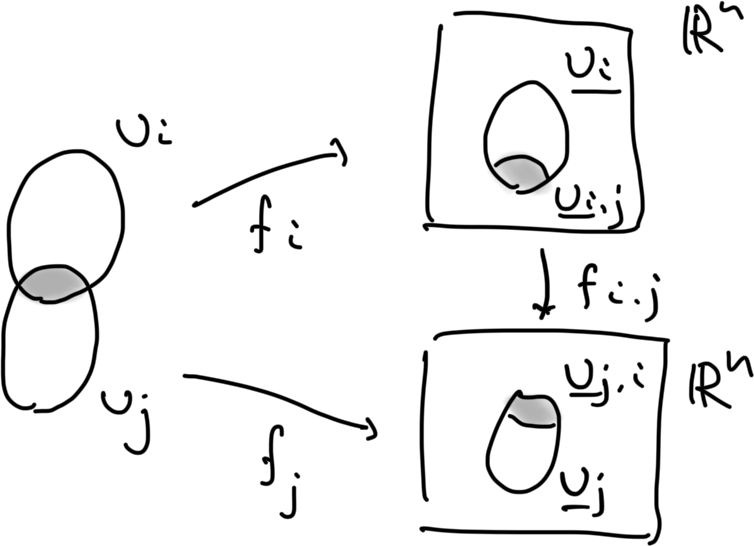
\includegraphics[scale=.3]{mfd.png} \]
\caption{Coordinate patches of a manifold \label{fig:coord-patch}}
\end{figure}

Suppose $U_i\cap U_j$ is nonempty. 
Let \begin{align}
\underline{U}_{i,j} &:= f_i(U_i\cap U_j) \subset \underline{U}_i,\\
\underline{U}_{j,i} &:= f_j(U_j\cap U_i)\subset \underline{U}_j.
\end{align}
Then we have the map \begin{equation}
f_{i,j} \colon \underline{U}_{i,j} \to \underline{U}_{j,i} 
\end{equation} defined by \begin{equation}
f_{i,j} := f_j \circ (f_i)^{-1} .
\end{equation}
This allows us to `paste together' $\underline{U}_i\subset \bR^n$ 
and $\underline{U}_j \subset \bR^n$
by identifying their subsets $\underline{U}_{i,j}$ and $\underline{U}_{j,i}$ using $f_{i,j}$.
%See Fig.~\ref{fig:pasting} for a drawing.


A smooth manifold is such that $f_{ij}$ are smooth;
a topological manifold is such that $f_{ij}$ are just required to be continuous.
A smooth manifold is automatically a topological manifold.
A bijective smooth map $f:M\to M'$ between two smooth manifolds $M$ and $M'$
is called a \emph{diffeomorphism};
a bijective continuous map $f:M\to M'$ between two topological manifolds $M$ and $M'$
is called a \emph{homeomorphism}.
In physics we typically consider smooth manifolds,
but I decided to include a bit of discussions about topological manifolds
as I thought the subtle concrete differences between smooth manifolds
and topological manifolds can be interesting to some of you.

\begin{theorem}
When a manifold $M$ is compact,
we can choose a finite number of coordinate patches $U_i$ to cover $M$.
\end{theorem}

Before going further, let us also introduce manifolds with boundaries:
\begin{definition}
  A \emph{manifold with boundary} is defined similarly,
  but we allow the neighborhood $\underline{U}$ to be in a half-space $\bR^{n-1}\times \bR_{\ge 0}$.
  The union of the inverse images of the boundary of 
  $\underline{U}\cap (\bR^{n-1} \times \{0\})$ 
  under $f$ is called \emph{the boundary of $M$}
  and is denoted by $\partial M$.
\end{definition}  

\begin{example}
  The half-space $\bR^{n-1}\times \bR_{\ge 0}$ is a manifold with boundary.
\end{example}

\begin{definition}
  A compact manifold without boundary is called a closed manifold.
\end{definition}


\subsection{Manifolds via equations}
So far we only saw trivial examples.
We need better examples.

\subsubsection{Generalities}
A common way to construct manifolds is to take a subset of $\bR^n$ defined by a number of equations:
\begin{align}
f_1(x_1, x_2, \ldots, x_n) &= 0, \\
f_2(x_1, x_2, \ldots, x_n) &= 0, \\
&\vdots \\
f_m(x_1, x_2, \ldots, x_n) &= 0.
\end{align}
If the choice of $f_{1,2,\ldots,m}$ are sufficiently nice,
the set of points satisfying these equations is a manifold of dimension $n-m$.

A typical bad example is the subset of $\bR^2$ defined by $xy=0$: around $(x,y)=(0,0)$, two lines intersect, and therefore the neighborhood of $(0,0)$ is not of the right form.

\subsubsection{Spheres and disks/balls}

\begin{example}
The $n$-dimensional sphere $S^n$ is defined by \begin{equation}
  x_1^2+x_2^2+\cdots+x_{n+1}^2=1.
\end{equation} 
\end{example}
Note that $S^n$ is embedded in $\bR^{n+1}$, but it is a manifold of dimension $n$.

\begin{example}
  The $n$-dimensional disk $D^n$ is defined by \begin{equation}
    x_1^2+x_2^2+\cdots+x_{n}^2\le 1.
  \end{equation} 
  This is a manifold with boundary, and the boundary is $S^{n-1}$.
  $D^n$ also called the $n$-dimensional ball and denoted by $B^n$.
\end{example}  

\begin{example}
$D^1$ is a segment $[-1,1]$ and its boundary $S^0$ consists of two points $\{-1,1\}$.
\end{example}

Calling two points, $S^0$, a 0-dimensional sphere sounds silly,
but it is just a name.
But this illustrates an important point:
you are not supposed to judge mathematical concepts by their names.
Rather, you are supposed to understand them by internalizing their definitions into your heart.

\begin{example}
  We can try considering points of constant Lorentz-invariant distance from the origin in $\bR^{d-1,1}$:
\begin{equation}
  x_1^2+x_2^2+\cdots+x_{d-1}^2-x_0^2=K ,
\end{equation}
where $K$ is a non-zero constant. 
This is a hyperboloid, and is a manifold of dimension $d-1$.
\end{example}
When $K>0$, it is connected; this is the hypersurface of spacelike-separated points 
of distance $\sqrt{|K|}$ from the origin
in the Minkowski spacetime.
When $K<0$, it consists of two components, one in the future $x_0>0$ and another in the past $x_0<0$.
They are the hypersurfaces of time-like separated points of temporal distance $\sqrt{|K|}$ from the origin.
When $K=0$, the equation above defines the lightcone, which is singular at the origin and is not a manifold.

\subsubsection{Group manifolds}
We have various group manifolds, 
defined in a similar manner.
 
Let $M_n(\bR)$ be the set of $n\times n$ real matrices.
\begin{example}
The orthogonal group $O(n)$ is defined by \begin{equation}
  O(n) = \{ M\in M_n(\bR) \mid M^T M = 1 \}.
\end{equation}
The special orthogonal group $SO(n)$ is defined by \begin{equation}
  SO(n) = \{ M\in O(n) \mid \det M = 1 \}.
\end{equation}
\end{example}

Similarly let $M_n(\bC)$ be the set of $n\times n$ complex matrices.
\begin{example}
The unitary group $U(n)$ is defined by \begin{equation}
  U(n) = \{ M\in M_n(\bC) \mid M^\dagger M = 1 \}.
\end{equation}
The special unitary group $SU(n)$ is defined by \begin{equation}
  SU(n) = \{ M\in U(n) \mid \det M = 1 \}.
\end{equation}
\end{example}

\begin{proposition}
$S^1=U(1)=SO(2)$.
\end{proposition}
This can be seen by parameterizing $S^1$ by $\theta \in [0,2\pi)$.
$U(1)$ is a one-by-one unitary matrix, i.e.~a complex number $z$ with $|z|=1$.
Therefore $z=e^{i\theta}$.
$SO(2)$ is a two-by-two orthogonal matrix with determinant $1$, which has the form \begin{equation}
  \begin{pmatrix}
    \cos\theta & -\sin\theta \\
    \sin\theta & \cos\theta
  \end{pmatrix}.
\end{equation}

\begin{proposition}
$S^3=SU(2)$.
\end{proposition}
This can be seen by noticing that any $SU(2)$ matrix has the form \begin{equation}
  \begin{pmatrix}
    z & -\overline w\\
    w & \overline z
  \end{pmatrix}
\end{equation} with $|z|^2+|w|^2=1$.
As $\bC^2\simeq \bR^4$, we see that this defines an $S^3$.
This fact can also be shown using quaternions $\bH$, 
introduced by Hamilton in 1843.
\begin{definition}
$\bH$ is a four-dimensional algebra over $\bR$ with a basis $1,i,j,k$ satisfying \begin{equation}
  i^2=j^2=k^2=-1, \quad
  ij=-ji=k, \quad
  jk=-kj=i, \quad
  ki=-ik=j.\label{eq:rel-of-H}
\end{equation}
\end{definition}

A general element is of the form $q=a+bi+cj+dk$ with $a,b,c,d\in \bR$.
The conjugate of $q=a+bi+cj+dk$ is $\bar q=a-bi-cj-dk$.
We can check that $\overline{q_1 q_2}=\bar q_2 \bar q_1$.

The norm of $q$ is $|q|^2=q\bar q=\bar q q=a^2+b^2+c^2+d^2$.
This is nonzero unless $q=0$.
This means that any nonzero element $q\neq 0$ has a multiplicative inverse $q^{-1}=\bar q/|q|^2$.
An algebra with this property is called a division algebra.
\begin{fact}
  The only finite-dimensional division algebras over $\bR$ are $\bR$, $\bC$, and $\bH$.
\end{fact}

Note also that $|q_1 q_2|^2=|q_1|^2 |q_2|^2$.
This means that the set $\{ q\in \bH \mid |q|=1 \}$ of unit quaternions forms a group.
As $\bH\simeq \bR^4$, this is a three-dimensional sphere $S^3$.
Considering $\bH\simeq \bC^2$, we can convince ourselves that this is also $SU(2)$.
More generally:
\begin{example}
  The unitary symplectic group $Sp(n)$ is defined by \begin{equation}
    Sp(n) = \{ M\in M_{n}(\bH) \mid M^\dagger M = 1 \}.
  \end{equation}
\end{example}
In particular, $Sp(1)=SU(2)=S^3$.
Note there is no distinct `special unitary symplectic group'.

To explain $Sp(m)$ a bit more geometrically, consider $\bH^n$
as the space of column vectors of quaternions. 
We consider `linear' maps  $M:\bH^n\to \bH^n$ in the sense that
\begin{equation}
M (vq) = (Mv) q, \qquad v\in \bH^n,\ q\in \bH.
\end{equation} 
(Note that the placement of $q$ on the right is important, 
as the multiplication is non-commutative in $\bH$.)
Denote the basis vectors by $e_1,e_2,\ldots,e_n$.
Then such an $M$ is specified by \begin{equation}
M e_i = \sum_j M_{ij} e_j.
\end{equation}
The condition $M^\dagger M=1$ is the condition that it preserves the norm $|v|$ of $v\in \bH^n$
defined by \begin{equation}
  |v|^2 := \sum_i |v_i|^2.
\end{equation}

\begin{fact}
  The only cases when $S^n$ is a group are $S^0=O(1)=\{1,-1\}$, $S^1=SO(2)=U(1)$
  and $S^3=SU(2)=Sp(1)$.
\end{fact}

Before moving on,
we also introduce the notations:
\begin{definition}
We use the notation $GL(n,\bK)$ for the group of invertible $n\times n$ matrices over a field $\bK$.
\end{definition}

\subsubsection{Time reversal and $\bR$, $\bC$, $\bH$}

Let me make a side remark concerning the natural role of $\bH$ in quantum mechanics.
Let's consider a quantum mechanical system with finite-dimensional Hilbert space $\cH$.
The time reversal operator $\sT$ is anti-unitary, in that 
\begin{equation}
  \sT z = \overline z \sT.
\end{equation}
Assuming that $\sT^2=c$ with a constant $c$, let's show $c=\pm1$. We evaluate $\sT^3$ in two orders:
\begin{equation}
\sT(\sT^2)= \sT c = \overline{c}\sT,\qquad
(\sT^2)\sT = c\sT.
\end{equation} Therefore $c=\overline{c}$. As the unitarity of $\sT^2$ requires $|c|=1$,
 we find $c=\pm 1$.

 \paragraph{The case $c=+1$:}
 This case, any vector $v\in \cH$ can be decomposed into its real and imaginary parts:
  \begin{equation}
    v = v_\text{re} + v_\text{im} i 
  \end{equation}
  where
  \begin{equation}
    v_\text{re}:= \frac{1+\sT}{2} v, \quad v_\text{im}:=\frac{1-\sT}{2i}v .
  \end{equation}
  Note that $T v_\text{re}= v_\text{re}$ and $T v_\text{im}=v_\text{im}$.
So, the $T$-invariant part of $\cH$ is a real vector space.
Denoting it by $\cH_\bR$, we see that if $\cH_\bR=\bR^n$, $\cH=\bC^n$.
Unitary matrices acting on $\cH$ commuting with $\sT$
are orthogonal matrices acting on $\cH_\bR$.
So, time-reversal-invariant unitary operators on $\cH$ 
form the group $O(n)$.

\paragraph{The case $c=-1$:}
In this case, we note that $i$, $j:=\sT$, $k:=i \sT$ satisfy 
the defining relation \eqref{eq:rel-of-H} of $\bH$.
(More precisely, we can equip the space $\cH$ of quantum states
with an action of $\bH$ from the right, via $vi := iv$ and $vj:=\sT v$.)

Therefore, $\cH= \bH^m$ for some $m$. When $\cH=\bC^n$, this forces $n=2m$ to be even.
This is known as Kramers degeneracy.

A unitary operator commuting with $\sT$
is a norm-preserving map on $\bH^m$ which commutes with the quaternion action from the right.
Therefore it belongs to $Sp(m)$.

\paragraph{Summary:}
$U(n)$, $SO(n)$, and $Sp(n/2)$ are the groups of norm-preserving linear operators
on a quantum system $\cH=\bC^n$ with $n$ states with the following conditions:
\begin{itemize}
\item $U(n)$: no time reversal,
\item $SO(n)$: time reversal with $\sT^2=+1$,
\item $Sp(n/2)$: time reversal with $\sT^2=-1$; $n$ is forced to be even.
\end{itemize}


\subsection{Manifolds via combinations}

Let's come back to the examples of manifolds.

\begin{notation}
 Given two manifolds $M$ and $N$ of dimensions $m$ and $n$,
 we write its product as $M\times N$.
It is a manifold of dimension $m+n$.
\end{notation}

\begin{notation}
Given two manifolds $M$ and $N$ of the same dimension $n$,
we write its disjoint union as $M\sqcup N$.
It is a manifold of dimension $n$.
\end{notation}

Note that $S^1\times S^1$ is two-dimensional and the surface of a donut,
while $S^1\sqcup S^1$ consists of two circles and is one-dimensional.

\begin{example}
  The $n$-dimensional torus is \begin{equation}
    T^n = \underbrace{S^1\times S^1\times \cdots \times S^1}_\text{ $n$ times}.
  \end{equation}
\end{example}

\begin{example}
$S^1\times [-1,1]$ is a cylinder. Its boundary is $S^1\sqcup S^1$.
\end{example}

Another construction is the following:
\begin{notation}
  Given two connected manifolds $M$, $N$ of dimension $n$,
  pick points $p\in M$ and $q\in N$.
  remove small open balls $B^n(p)$ and $B^n(q)$ from $M$ and $N$, and
  paste the common $S^{n-1}$ boundary.
  The result is the connected sum $M\# N$.
\end{notation}

For example, the connected sum 
\begin{equation}
  \underbrace{T^2 \# T^2 \# \cdots \# T^2}_\text{$g$ copies}
\end{equation}
is the surface of a multi-donut (whatever that is).
More professionally, it is called a genus-$g$ surface.
$S^2$ is defined to have genus 0.

\begin{fact}
Any two-dimensional compact connected oriented manifold is $S^2$ or 
the surface of a multi-donut with $g$ holes.
\end{fact}

\subsection{Manifolds via quotients}
\label{sec:quotient}
\subsubsection{Generalities}
Another method to define manifolds is to 
take the quotient of a manifold by a group action. 
Let us explain it more fully.
\begin{definition}
A \emph{group action} of a group $G$ on a manifold $M$ is a map \begin{equation}
  M\times G \to M, \quad (p, g) \mapsto p q
\end{equation} such that \begin{equation}
   p e = p, \quad  (p  g) h = p (gh)
\end{equation} for all $g,h\in G$ and $p\in M$.
Here $e$ is the identity in $G$.
We often abbreviate this situation by writing $M \curvearrowleft G$.
\end{definition}

More precisely, this is known as a right action of $G$.
We can similarly define a left action of $G$, so that 
we have $G\times M\to M$ satisfying $g(hp)=(gh)p$ instead.
We write $G\curvearrowleft M$ in this case.
In either case, we usually want the action to be smooth or at least continuous,
depending on the context.

Representations of groups on vector spaces are special cases:
\begin{definition}
  A representation $\rho$ of a group $G$ on a $\bK$-vector space $V$ is a group action (from the left) of $G$ on $V$, commuting with the scalar multiplication by $\bK$ (from the right).
  This means that for each $g\in G$, we have linear maps $\rho(g):V\to V$ such that $\rho(gh)=\rho(g)\rho(h)$.    
  We often abbreviate this situation by writing $\rho: G\curvearrowright V$.
\end{definition}

Let us now define the quotients:
\begin{definition}
For $p,q\in M$, let $p\sim q$ if there is a $g\in G$ such that $p g = q$.
The quotient space $M/G$ is the set $M/\sim$ of equivalence classes 
under this relation.
\end{definition}

$M/G$ is not always a manifold.
For example, consider $\bR^3$ with the action of $\bZ_2$ generated by 
\begin{equation}
(x,y,z) \mapsto (-x,-y,-z).
\end{equation}
The origin is singular, and the quotient space $\bR^3/\bZ_2$ is not a manifold.
(It still belongs to a larger class of spaces called \emph{orbifolds}.)
Actually, the quotient of a vector space by a group via its representation is almost never a manifold.
It is complicated to state the conditions under which $M/G$ is a manifold,
so we will not do so in this lecture series.

\subsubsection{Projective spaces}
We now define the real, complex and quaternionic projective spaces $\RP^n$, $\CP^n$ and $\HP^n$ uniformly.
\begin{example}
  \label{ex:proj}
  For $\bK=\bR,\bC,\bH$, 
  consider the action of $\bK\setminus \{0\}$ on
  $\bK^{n+1}\setminus\{0\}$ by scalar multiplication, (from the right when $\bK=\bH$).
  The projective space $\KP^n$ is then defined as
  \begin{equation}
    \KP^n = (\bK^{n+1}\setminus\{0\})/(\bK\setminus\{0\}).
  \end{equation}
  These are of dimension $n$, $2n$, and $4n$ respectively.
\end{example}
More directly, we consider elements 
\begin{equation}
(x_1,x_2,\ldots,x_{n+1})\in \bK^{n+1}
\end{equation} such that not all of $x_i$ is zero.
Then we make the identification \begin{equation}
  (x_1,x_2,\ldots,x_{n+1}) \sim  ( x_0, x_1, \ldots,  x_n)c \label{eq:proj-ident}
\end{equation} for nonzero $c\in \bK$.
A point on $\KP^n$,
which is an equivalence class under \eqref{eq:proj-ident},
is often denoted by \begin{equation}
  [x_1:x_2:\cdots:x_{n+1}].
\end{equation}

Before proceeding, we note that $\CP^n$ parameterize physically-distinct pure states 
in an $(n+1)$-dimensional Hilbert space.
Indeed, two nonzero ket vectors $\ket{\psi}$ and $\ket{\psi'}$ represent the same physical state
when there is a complex number $c$ such that $\ket{\psi'}=c\ket{\psi}$.
This is exactly the condition \eqref{eq:proj-ident}.

It is instructive to give explicit coordinate patches.
Let $U_i$ be the points on $\CP^n$ with $x_i\neq 0$.
Note that when $x_i\neq 0$, we have \begin{equation}
  (x_1,x_2,\ldots,x_{n+1}) \sim (x_1/x_i, x_2/x_i, \ldots, x_i/x_i=1, \ldots, x_{n+1}/x_i).
\end{equation} 
In other words, we can introduce coordinates on $U_i$ by defining  $y_k:=x_k/x_i$ for $k\neq i$;
equivalently, we constructed a map $f_i: U_i \to \underline{U}_i \simeq \bK^n$.

Let us consider another patch $U_j$ containing points with $x_j\neq 0$. 
We introduce coordinates $z_k:=x_k/x_j$ for $k\neq j$;
this gives the map $f_j: U_j \to \underline{U}_j\simeq \bK^n$.

$U_i$ and $U_j$ overlap when $x_i\neq 0$ and $x_j\neq 0$.
We then need to find the coordinate transformation 
between $f_i(U_i \cap U_j )\subset \underline{U}_i$
and $f_j(U_i \cap U_j) \subset \underline{U}_j$, realizing the identification of
\begin{equation}
  (y_1,y_2,\ldots,y_{n+1}) \quad \text{with $y_i=1$, $y_j\neq 0$}
\end{equation} and 
\begin{equation}
  (z_1,z_2,\ldots,z_{n+1}) \quad \text{with $z_j=1$, $z_i\neq 0$}.
\end{equation}
This is done by setting $z_k = y_k / y_j$, where $y_i$ was defined to be $=1$.

From this description we see \begin{equation}
\RP^1=S^1,\quad
\CP^1=S^2,\quad
\HP^1=S^4.
\label{eq:KP1}
\end{equation}
Indeed, in this case we have two patches \begin{equation}
  U_1 = \{ [1:y] \mid y\in \bK \}, \quad U_2 = \{ [z:1] \mid z\in \bK \}.
\end{equation} where $z=y^{-1}$ in the overlap $U_1\cap U_2$.
$U_1$ is the northern hemisphere,
$U_2$ is the southern hemisphere,
and they are patched to form a sphere in the appropriate dimensions.

Another way to look at $\KP^n$ is the following. 
To pick a representative under the identification \eqref{eq:proj-ident},
we first fix $\sum_i |x_i|^2 =1$.
As $\bK^{n+1}=\bR^{p(n+1)}$ where $p=1,2,4$ for $\bK=\bR,\bC,\bH$,
we have $S^n$, $S^{2n+1}$, $S^{4n+3}$ at this point.

The identification \eqref{eq:proj-ident} still acts within this sphere
if $|c|=1$. 
Depending on $\bK=\bR,\bC,\bH$, the group of such $c$ is $O(1)=\{\pm1\}=S^0$, $U(1)=S^1$, $Sp(1)=SU(2)=S^3$, respectively.
Therefore, we have \begin{equation}
\RP^n=S^n/O(1), \quad \CP^n=S^{2n+1}/U(1), \quad \HP^n=S^{4n+3}/Sp(1).
\label{eq:sphere-proj}
\end{equation}

\subsubsection{Homogeneous spaces}
\label{sec:homogeneous}
Another large class of quotient spaces
are the homogeneous spaces.
\begin{definition}
  \label{def:homogeneous-space}
  Given a subgroup $H\subset G$,
  introduce the equivalence relation $g_1\sim g_2$ if 
  there exists an $h\in G$ such that $g_1=g_2 h$.
  The quotient of $G$ by this relation is denoted by $G/H$,
  and is called a homogeneous space.
\end{definition}

A common way homogeneous spaces appear in physics is via symmetry breaking.
Say we have a configuration space $M$ (typically a vector space) acted on by a symmetry group $G$ from the left:
$M\ni m\mapsto gm\in M$ for $g\in G$.
Suppose we have a potential (or a free energy) $V:M\to \bR$ invariant under the $G$ action, i.e.~$V(gm)=V(m)$.
Suppose further that the potential has a minimum at $m_0 \in M$. 
From the $G$-invariance, all points of the form $gm_0$ are also minimum of $V$.
When the potential is generic, the space of the minimum of the potential is given by the orbit $Gm_0$.
Can we say more about the structure of this space?

Let $H\subset G$ be the subgroup fixing $m_0$, i.e.~$h\in H$ if and only if $hm_0=m_0$.
In such a situation, we say that the symmetry is broken from $G$ to $H$.\footnote{%
Physicists often write this as $G\to H$, 
but mathematically the map is in the opposite direction, $H\to G$.}
In this case $g_1 m_0 = g_2 m_0$ if and only if $g_2^{-1} g_1 \in H$, 
or equivalently $g_1 = g_2 h$ for some $h\in H$.
Therefore, we have $Gm_0=G/H$, i.e.~the space of the potential minimum is a homogeneous space
determined by the original symmetry $G$ and the unbroken symmetry $H$.

Note that mathematicians call the subgroup $H$ as the stabilizer of $m_0$,
whereas physicists usually call it the unbroken subgroup.

Let us give some examples.
We start with two trivial examples.
Let $G=SO(2)$ act on $(x,y)\in \bR^2$ by rotations.
A rotationally invariant potential $V(x,y)$ has the form
$V(x,y)=f(r)$ for $r^2=x^2+y^2$.
When the minimum is at $(x,y)=(0,0)$, its orbit under $SO(2)$ is a single point, $\{(0,0)\}$.
In this case the unbroken subgroup $H$ is the entirety of $SO(2)$.
So, we have $SO(2)/SO(2)=\{\text{point}\}$, a zero dimensional manifold consisting of a single point.
It is often abbreviated as $\pt$ in algebraic topology, so $SO(2)/SO(2)=\pt$.

When the minimum is at $(x,y)=(r_0,0)$ with $r_0\neq 0$,
its orbit under $SO(2)$ is the circle of radius $r_0$.
In this case the unbroken subgroup $H$ is $\{e\}$,
and $SO(2)/\{e\}=SO(2)$, which is a circle.
For an illustration, see Fig.~\ref{fig:winebottle}.

\begin{figure}[h]
\centering
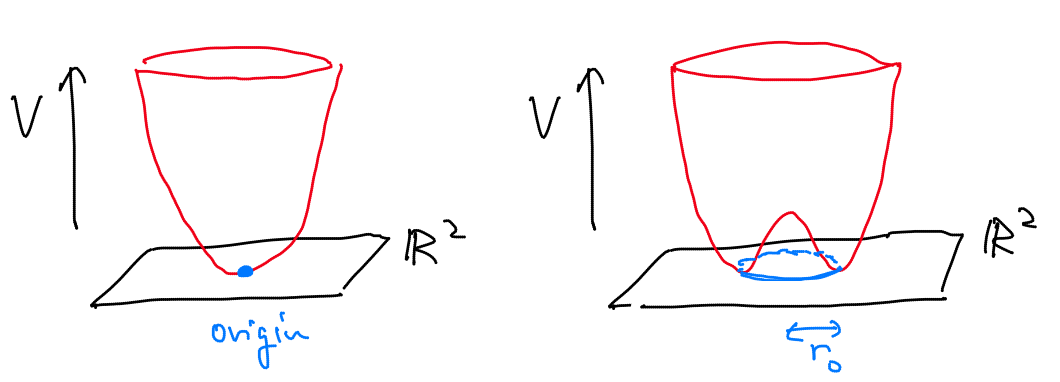
\includegraphics[width=.7\textwidth]{winebottle.png}
\caption{Two choices of $SO(2)$-invariant potential functions $V(x,y)$,
with minimum either at the origin or at the circle of radius $r_0$.}
\label{fig:winebottle}
\end{figure}

Let us generalize.
Let $SO(n)$ act on $\bR^n$ by rotations.
A rotationally invariant potential $V:\bR^n\to \bR$ 
has the form $V(x_1,\ldots,x_n)=f(r)$ where $r^2={x_1^2+\cdots+x_n^2}$.
When $f(r)$ has a minimum at $r_0>0$,
the space of the potential minimum is $S^{n-1}$ given by $x_1^2+\cdots + x_n^2=r_0^2$.

At $m_0=(r_0,0,\ldots,0)$, the subgroup of $SO(n)$ fixing $m_0$ is $SO(n-1)$.
Therefore, the space of the potential minimum is $SO(n)/SO(n-1)=S^{n-1}$.
Summarizing, we have found
\begin{proposition}
  \label{prop:SO/SO}
 $ SO(n)/SO(n-1) \simeq S^{n-1}$.
\end{proposition}

Let $U(n)$ act on $\bC^n$ by unitary transformations.
An invariant potential $\bC^n\to \bR$ has the form $V(z_1,\ldots,z_n)=f(r)$
where $r^2=|z_1|^2+\cdots+|z_n|^2$.
When $f(r)$ has a minimum at $r_0>0$,
the space of the potential minimum is $S^{2n-1}$ given by $|z_1|^2+\cdots + |z_n|^2=r_0^2$.

At $m_0=(r_0,0,\ldots,0)$, the subgroup of $U(n)$ fixing $m_0$ is $U(n-1)$.
Therefore, the space of the potential minimum is $U(n)/U(n-1)=S^{2n-1}$.
\begin{proposition}
  \label{prop:U/U}
$U(n)/U(n-1)\simeq S^{2n-1}$.
\end{proposition}

Let $Sp(n)$ act on $\bH^n$ in a standard manner.
By following the same logic as above, we get $Sp(n)/Sp(n-1)=S^{4n-1}$,
and we found that:
\begin{proposition}
  \label{prop:Sp/Sp}
$ Sp(n)/Sp(n-1)\simeq S^{4n-1}$.
\end{proposition}

Let us discuss a different but common example we see in quantum mechanics.
Consider an $n$-state system with the Hilbert space $\cH=\bC^n$.
The unitary group $U(n)$ acts on it.
On the observables, $g\in U(n)$ acts via \begin{equation}
  A\mapsto g A g^\dagger.
\end{equation}
Therefore, the subgroup $U(1) \subset U(n)$
consisting of scalar multiplications acts trivially: \begin{equation}
c A c^\dagger = A,
\end{equation} when $|c|=1$. 
What acts effectively on the space of observables is the quotient group $U(n)/U(1)$.

We note that $SU(n)\subset U(n)$ also acts on observables.
In this case, a scalar multiplication $c$ with $|c|=1$ is in $SU(n)$ if and only if $c^n=1$.
The complex numbers $\{c\mid c^n=1\}$ form a group isomorphic to $\bZ_n$,
and we found $\bZ_n \subset SU(n)$,
and the quotient $SU(n)/\bZ_n$ acts on the space of observables.

As any $U(n)$ matrix $U$ is of the form $c'U'$ for $c'\in U(1)$ and $U'\in SU(n)$,
we have $U(n)/U(1) = SU(n)/\bZ_n$.
This common quotient group is known as the projective unitary group, and denoted by $PU(n)$.
Summarizing, 
\begin{example}
The common quotient $U(n)/U(1)=SU(n)/\bZ_n$ is called the projective unitary group and is denoted by $PU(n)$.
\end{example}

For those who take wavefunctions as supreme, the natural symmetry group is $U(n)$,
whereas for those who take density matrices and/or observables as supreme,
the natural symmetry group is $PU(n)$.
This difference can produce subtle topological effects,
as we will see during this lecture series.

As our next example, 
let us consider the chiral symmetry breaking in QCD.
For simplicity let us consider the two-flavor case.
The symmetry $G$ is $SU(2)\times SU(2)$,
which acts on $\bC^2 \otimes \bC^2$,
where two $\bC^2$ factors are the standard two-dimensional representations of $SU(2)$.
A more convenient way to think about this action
is to regard $\bC^2\otimes \bC^2$ as the space of 
complex two-by-two matrices $M_2(\bC)$,
and to let $(g,g')\in SU(2)\times SU(2)$ to act on $m\in M_2(bC)$
via \begin{equation}
m\mapsto g m g'{}^{-1}.
\end{equation}

Say that $m$ takes the value $m=\mathbf{1}_{2\times 2}$.
The unbroken subgroup $H$ is formed by 
$\{(g,g)\}\subset SU(2)\times SU(2)$,
which is isomorphic to $SU(2)$ and is called the diagonal subgroup.
The orbit of $\mathbf{1}_{2\times 2}$ is simply 
the matrices of the form $gg'$,
i.e.~the subspace $SU(2)\subset M_2(\bC)$.
We thus found:
\begin{proposition}
We have $SU(2)\times SU(2)/SU(2)_\text{diagonal} = SU(2)$.
\end{proposition}


Our final example is the superfluid $^3$He;
its theory can be learned e.g.~in \cite{SuperfluidHe3Textbook,VolovikBook}.
It has a phase diagram as given in Fig.~\ref{fig:3He}.
\begin{figure}[h]
\centering
    \includegraphics[width=0.6\textwidth]{3He.pdf}
    \caption{Phase diagram of $^3$He (taken from \cite[Fig.7.1]{VolovikBook}).}
    \label{fig:3He}
\end{figure}
A $^3$He atom is a fermion with spin $1/2$, which can form a Cooper pair at low temperature.
There are two superfluid phases with zero magnetic field, known as the A phase and the B phase.
The order parameter (the expectation value of the Cooper pair) takes values in
$\bC^3\otimes \bC^3$,
where the first factor is for the spin angular momentum
and the second factor is for the orbital angular momentum,
both with spin 1.
Denote the basis vectors of the first $\bC^3$ by $\mathbf{e}_{1,2,3}$
and those of the second by $\mathbf{f}_{1,2,3}$.
The symmetry group $G$ of the free energy (neglecting a small spin-orbit coupling) is given by two separate $SO(3)$ actions on 
$\mathbf{e}_{1,2,3}$ and $\mathbf{f}_{1,2,3}$,
together with a common $U(1)$ phase rotation $\mathbf{e}_i \otimes \mathbf{f}_j \mapsto c\, \mathbf{e}_i \otimes \mathbf{f}_j$.
Therefore, we have \begin{equation}
  G = SO(3)\times SO(3)\times U(1)
\end{equation}
as the symmetry of the free energy.
\begin{example}
\label{ex:helium3}
In the superfluid phases of $^3$He, the order parameter takes the value
\begin{itemize}
\item $\mathbf{e}_1 \otimes (\mathbf{f}_2+ i\mathbf{f}_3)$ in the A phase,
\item $\sum_i \mathbf{e}_i \otimes \mathbf{f}_i$ in the B phase.
\end{itemize}
Denoting the subgroup preserved by these order parameters by $H_\text{A,  B}$,
the space of the potential minimum is given by $G/H_\text{A}$, $G/H_\text{B}$, respectively.
\end{example}

\begin{question}
Describe $H_\text{A}$ and $H_\text{B}$ as explicitly as possible.
\end{question}
You will see that the pattern of symmetry breaking is very similar to the 
breaking of the chiral symmetry in QCD.

With magnetic field, there is also a phase known as the A$_1$ phase.
The magnetic field reduces the symmetry of the free energy
to $SO(2)\times SO(3)\times U(1)$
and the order parameter takes the value 
 $(\mathbf{e}_2+i\mathbf{e}_3) \otimes (\mathbf{f}_2+ i\mathbf{f}_3)$.

We have one final question before moving on:
\begin{question}
Projective spaces are homogeneous spaces. Could you describe them as such?
\end{question}


\subsection{Non-orientable surfaces}

Let us now discuss some non-orientable manifolds.

\begin{example}
  Consider $S^1\times [-1,1]$, parameterized by $\theta\sim \theta+2\pi$ and $x\in [-1,1]$.
  We can consider the $\bZ_2$ action $(\theta,x)\mapsto (\theta+\pi,-x)$.
  The quotient space is called the M\"obius strip.
  This is non-orientable, and the boundary is a single circle $S^1$.
\end{example}

As a non-orientable closed manifold, 
we have $\RP^2$ we introduced above. To see this, recall $\RP^2=S^2/\bZ_2$,
where the $\bZ_2$ action identifies the antipodal points. 
Any point on the southern hemisphere is identified with some point on the northern hemisphere.
Then $\RP^2$ can be identified with the northern hemisphere
whose boundary, i.e.~the equator, has an extra identification $\theta \sim \theta+\pi$.

Let us have a closer look at the neighborhood of the equator.
We can parameterize it by the longitude $\theta$ together with the latitude $\phi\in (-\epsilon,\epsilon)$.
The antipodal identification is $(\theta,\phi)\sim (\theta+\pi,-\phi)$.
This is the same as the M\"obius strip, which is non-orientable.
In string theory, this local structure around the equator is called a crosscap (叉帽).
Another way to say this is that $\RP^2$ is obtained by pasting a northern hemisphere (i.e.~a disk)
to a M\"obius strip along the boundary.
Summarizing,
\begin{proposition}
$\RP^2$ is non-orientable.
\end{proposition}

Another non-orientable surface can be constructed by the following quotient:
\begin{example}
Consider $T^2$ parameterized by $\theta$ and $\phi$
with the identification $\theta\sim \theta+2\pi$ and $\phi \sim \phi+2\pi$,
and take a further identification as above: $(\theta,\phi)\sim (\theta+\pi,-\phi)$.
The result is known as the Klein bottle.
\end{example}
Locally around $\phi=0$ and $\phi=\pi$, we have two M\"obius strips.
So the resulting surface is obtained by pasting two M\"obius strips along the boundary.
Equivalently, it is obtained by taking the connected sum $\RP^2\#\RP^2$.

We can consider many other non-orientable surfaces by taking a repeated connected sum:
\begin{equation}
  \underbrace{\RP^2\#\RP^2\#\cdots\#\RP^2}_\text{$h$ copies}
  \#
  \underbrace{T^2\# T^2 \#\cdots\# T^2}_\text{$g$ copies}
\end{equation}
where we take $h>0$ and $g\ge 0$.
In fact, many of them are actually homeomorphic to each other.
\begin{fact}
Any compact connected non-orientable 2d surface is homeomorphic to
\begin{equation}
\RP^2 \# \underbrace{T^2\# T^2 \#\cdots\# T^2}_\text{$g$ copies}
\end{equation}
or the Klein bottle $\RP^2\#\RP^2$.
\end{fact}
It is a fun exercise to show that $\RP^2 \# \RP^2 \# \RP^2$ is homeomorphic to $\RP^2 \# T^2$.

\subsection{Some other fun manifolds}


\paragraph{The de-singularization of $\bC^2/\bZ_2$:}
Let's consider $\bC^2$ parameterized by $(z,w)$,
and consider the $\bZ_2$ action $(z,w)\mapsto (-z,-w)$.
The quotient space $\bC^2/\bZ_2$ is singular at the origin.
We can parameterize the same space in a different way:
Let $(s,t,u):=(z^2, z w, w^2)$.
Then the $\bZ_2$ action is trivial on $(s,t,u)$, but we have the relation $su=t^2$.
From $(s,t,u)$ satisfying $su=t^2$, we can uniquely reconstruct $(z,w)\simeq -(z,w)$.
So $\bC^2/\bZ_2$ can be identified with the subspace \begin{equation}
X=\{ (s,t,u)\in \bC^3 \mid su=t^2 \}.
\end{equation}
We can desingularize $X=\bC^2/\bZ_2$ in the following way.

We add the variables $(x_1,x_2)\in \bC^2\setminus \{0\}$, with the identification 
$(x_1,x_2)\sim a(x_1,x_2)$ for $a\in \bC\setminus \{0\}$,
i.e.~we introduce $\CP^1\simeq S^2$.
Recall that its points are denoted by $[x_1:x_2]$.
We now add a further constraint \begin{equation}
(z,w) = c(x_1,x_2) \quad \text{for some $c\in \bC$},
\end{equation} or equivalently \begin{equation}
  (s,t,u)= c'(x_1^2, x_1 x_2, x_2^2) \quad \text{for some $c'\in \bC$}. \label{eq:blowup}
\end{equation}

Denote the total space by $\tilde X$: 
it is a subspace of $\bC^3\times \CP^1$ 
parameterized by 
$(s,t,u,[x_1:x_2])$ 
under the constraints $su=t^2$ and \eqref{eq:blowup}.
This space comes with two projections maps, $\pi_1:\tilde X\to X=\bC^2/\bZ_2$ 
given by taking $(s,t,u)$
and $\pi_2:X\to \CP^1$ given by taking $[x_1:x_2]$.

Note that $\pi_1$ is one-to-one except at the origin, $(z,w)=(0,0)$.
It is because the relation \eqref{eq:blowup} uniquely determines $[x_1:x_2]=[z:w]$.
At the origin, $(z,w)=(0,0)$, the inverse image is the entirety of $\CP^1$. 
So, $\tilde X$ can be thought of inserting  $\CP^1$ at the origin of $X=\bC^2/\bZ_2$.

$\tilde X$ is actually a smooth manifold.
To see this, we consider the second projection $\pi_2: \tilde X\to \CP^1$.
Given a point $[x_1:x_2]\in \CP^1$,
the inverse image of $\pi_2$ is simply $c'(x_1^2, x_1 x_2, x_2^2)\in \bC$
for $c'\in \bC$. 
So it is isomorphic to a copy of $\bC$.
So $\tilde X$ can be visualized as a copy of $\bC$ attached smoothly at each point of $\CP^1$,
and is a smooth manifold.
This is an example of a fiber bundle we discuss in the next section.

\paragraph{A K3 manifold:}

The manifold $\tilde X$ introduced above was non-compact. 
It can be used to construct a rather important compact manifold of dimension 4.
We start from $T^4$ parameterized by $\theta_i\in \bR$ with the identification $\theta_i\sim \theta_i+2\pi$, for $i=1,2,3,4$.
We consider the $\bZ_2$ action given by \begin{equation}
  (\theta_1,\theta_2,\theta_3,\theta_4) \mapsto -(\theta_1,\theta_2,\theta_3,\theta_4).
\end{equation}
Note that we have $\theta \sim -\theta$ under the identification $\theta\sim \theta+2\pi$ if and only if $\theta=0,\pi$.
The quotient space $T^4/\bZ_2$ is therefore singular at $2^4=16$ points
when $\theta_i = 0,\pi$ for $i=1,2,3,4$.
Around each point, it locally has the form $\bR^4/\bZ_2 = \bC^2/\bZ_2$ studied above.
Then, we can insert 16 copies of $\CP^1$ at these 16 points to desingularize the space.
The result is a smooth compact manifold of dimension 4, 
and is an example of a class of manifold called K3.\footnote{%
The name K3 was introduced by the mathematician A. Weil, after the three mathematicians 
Kummer, K\"ahler, and Kodaira who studied it, and also the mountain K2 in the Himalayas.
The construction given here is due to Kummer.
}

\subsection{Some curious facts about manifolds}
\label{sec:smooth-vs-topological}

\subsubsection{Smooth vs.~topological manifolds}
Consider the following equation in $\bC^5$:
\begin{equation}
z_1^2+z_2^2+z_3^2+z_4^3+z_5^{6k-1}=0.  
\end{equation} Except at the origin, it is a smooth manifold of complex dimension 4, 
i.e.~of real dimension 8.
We can take the intersection with the unit sphere $S^9=\{\sum|z_i|^2=1\}$ in $\bC^5$.
This results in a smooth compact manifold $M_k$ of dimension 7.
It is known that $M_k$ are all homeomorphic to the standard $S^7$,
but they are not diffeomorphic to it unless $k$ is a multiple of $28$.
In fact, there are exactly 28 ways to make $S^7$ into a smooth manifold,
and the construction above exhausts them.
This goes back to Milnor in 1956; a very readable account is given e.g.~in \cite{MeerThesis}.
These manifolds are called exotic spheres, 
but they are not very exotic, as the explicit equation above shows!

There are also cases where a topological manifold does not admit any smooth structure.
That there are such manifolds in four dimensions was realized by Freedman \cite{Freedman} in 1982.
An example is called as the $E_8$ manifold.
Again the construction with coordinate patches with continuous maps between them is explicit;
what was difficult was to show that there cannot be any smooth structure. 
Next year in 1983, Donaldson \cite{Donaldson} 
introduced a new method to study smooth four-dimensional manifolds
using gauge theory, with many spectacular results.
One result which was soon found is that $\bR^4$ also has a smooth structure 
which is not diffeomorphic to the standard one.
(For example, in one of such exotic smooth structures, 
any smoothly embedded $S^3$ in it resides in a compact region around the origin.
So, there can't be an arbitrarily large $S^3$ in it.)

\subsubsection{Triangulation of manifolds}
Two-dimensional surfaces can be triangulated. 
We can ask the same question in higher dimensions,
where we replace triangles by simplices. (A simplex in dimension $n$ has $n+1$ vertices, etc.)
Can manifolds be triangulated?
It is known that smooth manifolds can be triangulated. 
How about topological manifolds?

Well, the four-dimensional $E_8$ manifold above cannot be triangulated.
The situation in dimensions more than five was more subtle.
It was shown by Matumoto \cite{Matumoto} in 1978 and Galewski-Stern \cite{GalewskiStern} in 1980 that,
all topological manifolds of dimension $n\ge 5$ can be triangulated
\emph{if} there exists a \emph{three}-manifold satisfying certain properties.
If no such three-dimensional manifold exists,
then for every dimension $n\ge 5$ there are topological manifolds which cannot be triangulated.
Non-existence of such a three-manifold was finally proved by Manolescu \cite{Manolescu} in 2013.
This work used a mathematical version of Seiberg-Witten theory,
which originated in the study of supersymmetric gauge theory 
in theoretical physics by Seiberg and Witten in the mid-1990s,
who showed how confinement happens in a supersymmetric version of QCD.
This mathematical Seiberg-Witten theory 
can be considered as an easier version of Donaldson's theory referred to above,
and has been developed vigorously by mathematicians since its introduction.


\subsubsection{Some comments}
So we have hierarchy of structures on manifolds: \begin{multline}
  \{\text{topological manifolds}\}
  \supset
  \{\text{triangulated manifolds}\} \\
  \supset
  \{\text{PL manifolds}\}
  \supset
  \{\text{smooth manifolds}\}
\end{multline}
where I added another stage, known as piecewise-linear (PL) manifolds,
which can be found more often discussed in the math literature 
than triangulated manifolds.\footnote{%
PL manifolds are triangulated manifolds such that
for each vertex $v$, the link of $v$ (the polyhedron formed by 
simplices immediately surrounding $v$) is piece-wise-linear isomorphic to $S^{n-1}$.
}
There are various differences at each stage, as we have seen above.

Why do we/I care about these things?
I don't really know.  But let me give some excuses.
\begin{itemize}
  \item Firstly, it's simply interesting, at least to me.
\item Secondly, it is particularly interesting that gauge-theoretic (and therefore physics-inspired)
methods were used to study these issues.
\item Thirdly, I found the following difference between hep-th and cond-mat people:
In hep-th, we often consider smooth manifolds as given (as in general relativity),
whereas in cond-mat, manifolds only appear as long-range approximation of a more fundamental
lattice structure. 
In theoretical condensed-matter physics, a general manifold is often studied
assuming that it is equipped with a triangulation. 
Therefore, I think that it might be of some use to be aware of the distinction between
these two approaches to manifolds.
For example, it seems possible to write down
the Hamiltonian of a strange symmetry-protected topological phase
which is defined on triangulated manifolds such that
it detects non-smooth but triangulable manifolds, 
using a characteristic class known as the Kirby-Siebenmann class.
This results in a model in a rather high dimensionality meaningless in our actual world, though.
\end{itemize}

\section{Fiber bundles}

After having seen some explcit examples of manifolds,
let us move on to the study of fiber bundles,
which are a kind of twisted products of manifolds.

\subsection{Definition}

\begin{definition}
A fiber bundle is the data of a map $p: E\to B$
where $E$ and $B$ are manifolds,
such that there is a fixed manifold $F$ so that
for each $b\in B$ we have a neighborhood $b\in U\subset B$ 
and a bijective map $f: p^{-1}(U)\to U\times F$
that is compatible with the projection, i.e.~the following diagram \begin{equation}
  \begin{array}{ccc}
    p^{-1}(U) & \xrightarrow{f} & U\times F \\
    \downarrow & & \downarrow \\
    U & = & U
  \end{array}
\end{equation}
commutes, where the down arrows are projections.
$F$, $E$ and $B$ are called the fiber, total space, and base space, respectively.
The map $f$ above is called a local trivialization.
\end{definition}

In other words, a fiber bundle over $B$ with fiber $F$
can be built by first covering $B$ by open sets $U_i$,
taking the product $U_i \times F$ for each $i$,
and we glue them over the overlaps $U_{ij}:=U_i\cap U_j$ via
maps $f_{ij}$ as follows:
\begin{equation}
  \begin{array}{cccccccc}
    U_i \times F &\supset& U_{ij}\times F & \xrightarrow{f_{i,j}} & 
    U_{ij}\times F & \subset & U_j\times F \\
    \downarrow & & \downarrow & & \downarrow & & \downarrow \\
    U_i & \supset & U_{ij} & = & U_{ij} & \subset & U_j
  \end{array}
\end{equation}
where all the down arrows are the projections forgetting the fiber direction.

\begin{notation}
  As a shorthand, we often refer to a fiber bundle as 
  \begin{equation}
  F\stackrel{\iota}{\longrightarrow} E\stackrel{p}{\longrightarrow} B.  
  \end{equation}  
  Here, $\iota$ is the inclusion of the fiber over a point $b$ in the base $B$.
\end{notation}

%\begin{remark}
In algebraic topology, there is a more general concept called a \emph{fibration}, which is denoted similarly: $F\to E\to B$.
A fiber bundle is a fibration, but a fibration is not necessarily a fiber bundle.
%\end{remark}

\begin{definition}
  \label{def:bundle-equiv}
Two fiber bundles $F\to E\xrightarrow{p} B$ and $F\to E'\xrightarrow{p'} B$ with the same fiber
are said to be equivalent if there is a bijection $f: E\to E'$ 
compatible with the projections, i.e.~the following diagram commutes:
\begin{equation}
  \begin{array}{ccc}
    E & \xrightarrow{f} & E' \\
    \downarrow & & \downarrow \\
    B & = & B
  \end{array}
\end{equation}
where the down arrows are projections $p$ and $p'$.
\end{definition}

\begin{example}
  The product $E = B\times F$ is a fiber bundle over $B$ with fiber $F$.
\end{example}

\begin{figure}[h]
  \[
    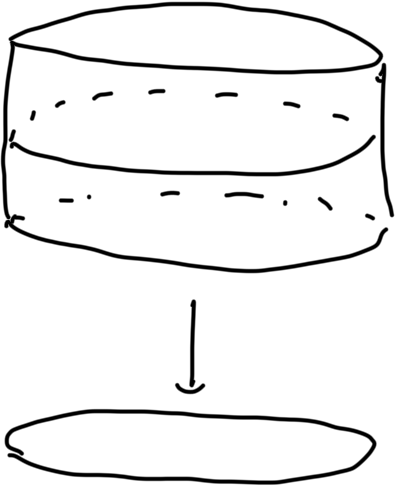
\includegraphics[width=0.2\textwidth]{cylinder.png}
    \qquad
    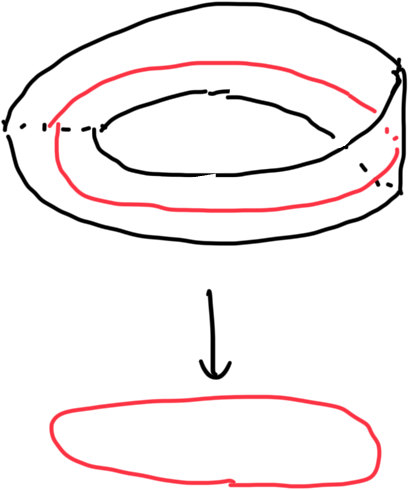
\includegraphics[width=0.2\textwidth]{mobius.png}
  \]
    \caption{A cylinder and a M\"obius strip.}
    \label{fig:cyl-mob}
\end{figure}

\begin{example}
A cylinder $S^1\times [-1,1]$ is a fiber bundle over $S^1$ with fiber $[-1,1]$.
\end{example}

\begin{example}
A M\"obius strip is a fiber bundle over $S^1$, where the fiber is the segment $[-1,1]$.
\end{example}

\noindent See Fig.~\ref{fig:cyl-mob} for my terrible drawings.


A cylinder and a M\"obius strip are inequivalent,
although the fiber and the base of both cases are the same.
One way to see this is to note that the boundary of 
the cylinder is $S^1\sqcup S^1$, while the boundary of the M\"obius strip is $S^1$.
Developing more general methods to distinguish different fiber bundles
with the same fiber and the same base is one of the goals
of the study of fiber bundles.

\subsection{Principal $G$-bundles}
\subsubsection{Generalities}
\begin{proposition}
  \label{prop:free-quotient}
Suppose $G$ acts on a manifold $M$.
We further suppose that this action is free,
i.e.~for each $m\in M$ the only $g\in G$ such that $mg=m$ is $g=e$.
Then the projection $p: M\to M/G$ is a fiber bundle with fiber $G$.
In other words, we have a fiber bundle $G\to M\to M/G$.
\end{proposition}

In this description it can be said that we are giving the total space $M$ 
more importance than the base $M/G$.
If we consider the base $B=M/G$, as the primary object, we get to the following viewpoint:

\begin{definition}
  \label{def:principal-bundle}
  A fiber bundle $p: P\to B$ with fiber $G$ is called a principal $G$-bundle
  if $P$ is equipped with an action of $G$ from the right, such that 
  for each $b\in B$ we have $U\subset B$ so that we have
  the following identification compatible with the $G$ action:
  \begin{equation}
  \begin{array}{ccc}
    p^{-1}(U) & \simeq & U\times G \\
    \downarrow & & \downarrow \\
    U & = & U
  \end{array} .
  \end{equation}
\end{definition}


Now, the total space $P$ is built 
as before by gluing $U_i\times G$ and $U_j\times G$ over $U:=U_i \cap U_j$ as 
\begin{equation}
  \begin{array}{cccccccc}
    U_i \times G &\supset& U\times G & \xrightarrow{f_{ij}} & 
    U\times G & \subset & U_j\times G \\
    \downarrow & & \downarrow & & \downarrow & & \downarrow \\
    U_i & \supset & U & = & U & \subset & U_j
  \end{array}
\end{equation}
where $f_{ij}$ has to be compatible with the right action of $G$.
Let us make $f_{ij}$ more explicit.

For this we need to use the following tautological lemma:
\begin{lemma}
A map $f:G\to G$ compatible with the right $G$ action is given by 
a left multiplication by an element $g\in G$, $f(h)=gh$.
\end{lemma}
Indeed, we need to have $f(h_1 h_2) = f(h_1) h_2$.
Therefore $f(h)=f(eh)=f(e)h$. Defining $g:=f(e)$, we have $f(h)=gh$.
This completes the proof.

Using this lemma at each point $b\in U$,
we find that  $f_{ij}: U\times G\to U\times G$ is given explicitly by
\begin{equation}
  f_{ij}: (b,g) \mapsto (b, g_{ij}(b) g)
  \label{eq:principal-bundle-transition-function}
\end{equation}
by a function $g_{ij}: U\to G$.

When is a principal $G$-bundle $P\to B$ equivalent to the trivial bundle $B\times G \to B$?
By definition this means that there is a bijective map $h: P\to B\times G$
compatible with the projections and the $G$ action from the right.
On each patch $U_i$, $h$ is given by $f'_i: p^{-1}(U_i)\to U_i\times G$
compatible with the $G$ action and the projection.
Using the above lemma again,
it is determined by a map $g'_i: U_i\to G$ via $f'_i(b,g)=(b,g'_i(b)g)$.
Furthermore, these maps $g'_i$ must be compatible with the patching procedure, i.e.~the following diagram must commute:
\begin{equation}
\vcenter{\xymatrix{
  G \ar[r]^{g_{ij}} \ar[d]_{g'_i} & G \ar[d]^{g'_j} \\
  G \ar[r]^{\text{id}} & G 
}},
\end{equation}
i.e.~$g_{ij} = (g'_j)^{-1} g'_i$.
Summarizing, we found: 
\begin{proposition}
  A principal $G$-bundle $P\to B$
  given in terms of \eqref{eq:principal-bundle-transition-function}
  is equivalent to the trivial principal $G$-bundle $B\times G \to B$
  if and only if there are maps $g_i: U_i\to G$ such that $g_{ij} = (g_j)^{-1} g_i$.
\end{proposition}

\subsubsection{Examples}

Now many of the examples we saw in Sec.~\ref{sec:quotient} can be rephrased as principal bundles.
In particular, the equation \eqref{eq:sphere-proj} means the following:
\begin{example}
  \label{ex:RPn}
$S^n\to \RP^n$ is a principal $O(1)=\bZ_2$-bundle.
\end{example}

\begin{example}
  \label{ex:CPn}
$S^{2n+1}\to \CP^n$ is a principal $U(1)=S^1$-bundle.
\end{example}

\begin{example}
  \label{ex:HPn}
  $S^{4n+3}\to \HP^n$ is a principal $Sp(1)=SU(2)=S^3$-bundle.
\end{example}

Furthermore, we saw that $\RP^1=S^0$, $\CP^1=S^2$, $\HP^1=S^3$ 
in \eqref{eq:KP1}. 
This means that we have the following fiber bundles:
\begin{itemize}
  \item $\bR^2\supset S^1\to \RP^1=S^1$  is an $S^0$ bundle,
  \item $\bC^2\supset S^3\to \CP^1=S^2$ is an $S^1$ bundle,
  \item $\bH^2\supset S^7\to \HP^1=S^4$ is an $S^3$ bundle.
\end{itemize}

These are known as Hopf fibrations.
These bundles are nontrivial
and are different from a product.
For example, in the second case,
the total space is $S^3$,
which is different from $S^2\times S^1$,
the total space of a trivial $S^1$ fiber bundle over $S^2$.
(Note that we haven't actually learned how to distinguish
$S^3$ and $S^1\times S^2$.
This we will do later.)

We have a few comments.
\begin{itemize}
\item The first example is a 2:1 map,
already drawn in Fig.~\ref{fig:cyl-mob} 
as a map from the boundary $S^1$ of the M\"obius strip to the base $S^1$.
\item The second example can be given a different description. 
Regard $S^3$ as parameterizing norm-one states
in a qubit:
\begin{equation}
  \ket{\psi}=\begin{pmatrix}u \\v \end{pmatrix},
  \qquad (|u|^2+|v|^2=1).
\end{equation}
Now form the expectation values of Pauli matrices:
\begin{align}
  x &:= \bra{\psi} \sigma_X \ket{\psi} = \bar u v + \bar v u, \\
  y &:= \bra{\psi} \sigma_Y \ket{\psi} = -i\bar u v +i \bar v u, \\
  z &:= \bra{\psi} \sigma_Z \ket{\psi} = |u|^2 - |v|^2.
\end{align}
It is straightforward to check that $x^2+y^2+z^2=1$.
Therefore the map \begin{equation}
(u,v)\mapsto (x,y,z)
\label{eq:uvXYZ}
\end{equation} defines a map \begin{equation}
  S^3\to S^2.
\end{equation}
That the fiber of this map is an $S^1$ is clear from the fact
that the expectation values are invariant under the change
$\ket{\psi}\mapsto c\ket{\psi}$ where $|c|=1$.
The sphere $S^2$ parameterized by $(x,y,z)$ is often referred to as the Bloch sphere of the qubit.\footnote{%
The history behind this terminology is quite interesting.
It originates in \cite{ACGT}, a paper about quantum optics,
where the authors refer to a work of Felix Bloch on nuclear magnetic resonance \cite{Bloch}, 
although this particular paper by Bloch does not study at all the Bloch sphere as we know it.
This was then adopted by the quantum information community,
which then became a standard terminology more generally, due to the increasing popularity of qubits. 
(I used \url{https://physics.stackexchange.com/questions/636913/} as a source.)
}
We can also give a more explicit parameterization of the map above:
\begin{equation}
  \label{eq:Hopf-explicit}
(\cos(\theta/2)  e^{i \psi},
\sin(\theta/2) e^{i(\phi+\psi)} )
\mapsto  (\sin\theta\cos\phi,\sin\theta\sin\phi,\cos\theta).
\end{equation}
This shows that the fiber above a point on $S^2$ is parameterized by $\psi$.

We can stereographically project points on $S^3$ to $\bR^3$ via \begin{equation}
(a,b,c,d) \mapsto \frac{1}{1-a}(b,c,d),
\end{equation} see Fig.~\ref{fig:stereo}.
Using this, we can draw the fibers of each point on $S^2$ as circles within $\bR^3$.
In Fig.~\ref{fig:hopf-fibers}, I drew the fibers of $(\cos 2\pi k/8, \sin 2\pi k/8, 0)$ for $k=0,1,\ldots,7$ in this manner.
\begin{figure}[h]
\centering   
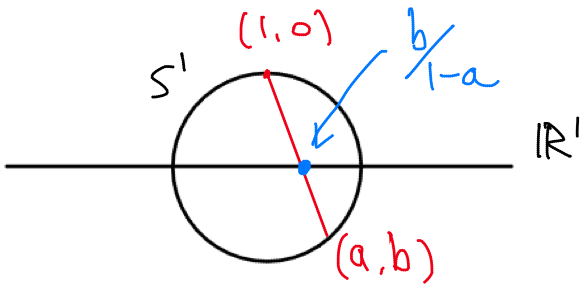
\includegraphics[width=0.3\textwidth]{stereo.png}
  \caption{Stereographical projection from $S^3$ to $\bR^3$}
  \label{fig:stereo}
\end{figure}
\begin{figure}[h]
\centering   
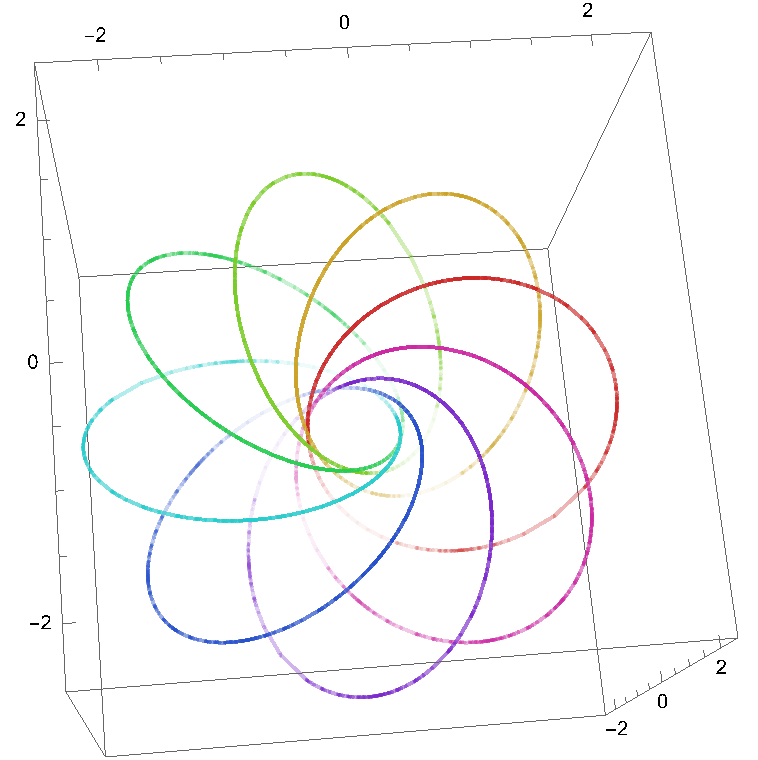
\includegraphics[width=0.5\textwidth]{hopf-fibers.png}
  \caption{Fibers of the Hopf fibration, drawn after a stereographic projection.}
  \label{fig:hopf-fibers}
\end{figure}

\item All the three fibrations above have the form
$S^n \to S^m \to S^{m-n}$.
One wonders if there are other examples of this form.
Actually we have:
\end{itemize}

\begin{fact}
These three Hopf fibrations, together with a final one
$S^7\to S^{15}\to S^8$
 exhaust 
such fibrations $S^n\to S^m\to S^{m-n}$.
\end{fact}
The last one, related to octonions, is not a principal fiber bundle, since $S^7$ is not a group.

We can also use the fact that Hopf fibrations are nontrivial to show that
the fibrations given in Examples \ref{ex:RPn}, \ref{ex:CPn}, \ref{ex:HPn} 
are all nontrivial.
Let us show this in the case of $\RP^n$. For this, we consider the following commutative diagram:
\begin{equation}
\begin{array}{ccccc}
  \bZ_2 &\to& S^n &\to& \RP^{n}  \\
   \rotatebox{90}{$=$} & & \cup & & \cup \\
    \bZ_2 &\to& S^1 &\to& \RP^1
\end{array}.
\end{equation}
Here, $S^1\subset S^n$ is obtained by restricting most of the coordinates to be zero.
We already saw that the second line is a nontrivial fibration.
As the first line contains the second line, the first line is also nontrivial.
Summarizing, we have: 
\begin{proposition}
  \label{prop:nontriviality-projective-fibration}
  The fibrations $\bZ_2\to S^n\to \RP^n$,
  $S^1\to S^{2n+1}\to \CP^n$,
  $S^3\to S^{4n+3}\to \HP^n$
  are all nontrivial.
\end{proposition}

The homogeneous spaces, introduced in Definition~\ref{def:homogeneous-space}
with many examples below it,
also give rise to principal bundles.
\begin{proposition}
  $G$ is a principal $H$-bundle over $G/H$, i.e.~we have a fiber bundle $H\to G\to G/H$.
\end{proposition}

Let us give an example not directly treated in Section~\ref{sec:homogeneous}.
Consider $g\in SU(2)$ acting on $\bC^2$.
Note that $2\times 2$ traceless Hermitean matrices are paramaterized by $\bR^3$,
by $x\sigma_x+y\sigma_y+z\sigma_z$.
We let $g\in SU(2)$ acts on this space via \begin{equation}
R_g: (x,y,z) \mapsto (x',y',z')  \label{eq:Rg1}
\end{equation} where \begin{equation}
g(x\sigma_x+y\sigma_y+z\sigma_z)g^\dagger = x'\sigma_x+y'\sigma_y+z'\sigma_z.
\label{eq:Rg2}
\end{equation}

An function $V:\bR^3\to \bR$ invariant under this $SU(2)$ action 
has the form $V(x,y,z)=f(r)$ where $r^2={x^2+y^2+z^2}$.
Suppose $f(r)$ has a minimum at $r_0>0$.
The space of the potential minimum is $x^2+y^2+z^2=r_0^2$, which is a sphere $S^2$.
Take $m_0=(0,0,r_0)$, corresponding to $r_0 \sigma_z$.
The elements of $SU(2)\simeq S^3$ fixing this point have the form $e^{i\theta \sigma_z}$ for some $\theta$,
and is isomorphic to $U(1)\simeq S^1$.
In this way we again found \begin{equation}
  S^1 \to S^3 \to S^2.
\end{equation}
This symmetry breaking pattern was first introduced by Georgi and Glashow in the context of the electroweak theory \cite{Georgi:1972cj}.
Although it does not match the experimental results,
it still serves as a model simpler than the reality (the Standard Model),
where we can practice our techniques. 
It will play an important role in our analysis of monopoles later, too.

Note that we have defined a map $SU(2)\to SO(3)$ by $g\mapsto R_g$ where $R_g$ was given in \eqref{eq:Rg1} and \eqref{eq:Rg2}.
This is a homomorphism, and the kernel is $\{\pm 1\}$.
In other words we have found:
\begin{example}
  There is a fiber bundle $
    \{\pm 1\} \to SU(2) \to SO(3). 
  $
\end{example}
Recalling that $SU(2)\simeq S^3$, we also see that 
\begin{proposition}
$SO(3)\simeq \RP^3$.  
\end{proposition}

Note that this is simply an example of the fibration $\bZ_2\to S^n\to \RP^n$
for $n=3$,
which therefore is nontrivial, as we already saw in Proposition~\ref{prop:nontriviality-projective-fibration}.

\subsection{Vector bundles}

Another large class of bundles is given by the vector bundles,
where the fiber is a vector space.

\begin{definition}
  Pick the field of scalars $\bK$ to be either $\bR$, $\bC$ or $\bH$.
  A vector bundle is a fiber bundle $E\to B$ with fiber $V$,
  where $V$ is a vector space, such that two local trivializations over $U_i \subset B$
  and $U_j\subset B$ are related in the following manner on the overlap $U:=U_i\cap U_j$:
  \begin{equation}
  \begin{array}{cccccccc}
    U_i \times V &\supset& U \times V & \xrightarrow{f } & 
    U \times V & \subset & U_j\times V \\
    \downarrow & & \downarrow & & \downarrow & & \downarrow \\
    U_i & \supset & U  & = & U  & \subset & U_j
  \end{array}
  \end{equation}
  where $f $ is given by \begin{equation}
    f : (b,v) \mapsto (b, g (b) v)
    \label{eq:vec-bundle-transition-functions}
  \end{equation} where $g (b): V\to V$ is a linear map smoothly depending on $b\in U$.
  The dimension of $V$ is called the rank of the vector bundle.
\end{definition}
$\bR$-vector bundles, $\bC$-vector bundles, and $\bH$-vector bundles
are also called real, complex, and quaternionic vector bundles, respectively.

In physics it is also common to have an inner product on the fibers $V$ of a vector bundle,
so that the transition functions $g (b)$ are not just linear maps
but in $O(n)$, $U(n)$, or $Sp(n)$, respectively.
We will come back to this point later.


\begin{definition}
  A section of a vector bundle $p:E\to B$ is a map $\psi: B\to E$ such that $p\circ \psi $ is the identity map on $B$.
\end{definition}
More informally, $\psi(b)$ for $b\in B$ takes values in the fiber $V$ over $b$.
Sections of vector bundles appear in physics usually in one of the two ways:
\begin{itemize}
  \item As fields, where the base space $B$ is spacetime and 
  the fiber $V$ is the possible values the fields can take.
  This appears ubiquitously in hep-th, in the gauge theory setting.
  The metric tensor in general relativity is also a section of a vector bundle.
  \item As wavefunctions of a quantum mechanical system, 
  where the system can be separated 
  into the degrees of freedom along the base space $B$
  and additional degrees of freedom parameterized by the fiber $V$ 
  which is the Hilbert space of a quantum subsystem.
  This arise, for example, in the Born-Oppenheimer approximation,
  where $B$ is for the slow motion of some degrees of freedom (such as the position of the nuclei) and 
  $V$ is for the fast motion of other degrees of freedom (such as electrons).
  It can also arise in the study of crystalline materials,
  where $B$ is the Brillouin zone and $V$ is the spaces of quantum states at fixed wave number.
\end{itemize}

\begin{definition}
A vector bundle whose fiber is one dimensional over $\bK$ is called a 
$\bK$-line bundle.
Here $\bK$ is either $\bR$, $\bC$ or $\bH$.
\end{definition}
Most often, a line bundle refers to a complex line bundle, i.e.~a vector bundle
whose fiber is a one-dimenisonal complex vector space.\footnote{%
I think mathematicians are crazy in that they call the space of complex numbers a `line'.
}

When we have two vector spaces $V$ and $W$,
we can form the direct sum $V\oplus W$ or the tensor product $V\otimes W$.
These operations can be lifted to vector bundles,
by performing them fiberwise.
\begin{definition}
  Given two vector bundles $E\to B$ and $E'\to B$ with fibers $V$ and $W$,
  we can form the direct sum $E\oplus E'$ over $B$ with fiber $V\oplus W$,
  or the tensor product bundle $E\otimes E'$ over $B$ with fiber $V\otimes W$.  
\end{definition}

Given a vector space $V$, the space of linear functions $V\to \bK$ is denoted by $V^*$
and is also a  vector space.
Doing this fiberwise, we have:
\begin{definition}
  Given a vector bundle $E\to B$ with fiber $V$,
  we can form the dual bundle $E^*\to B$ whose fiber is $V^*$.
\end{definition}
Similarly, for a complex vector bundle, we can do:
\begin{definition}
  Given a complex vector bundle $E\to B$ with fiber $V$,
  we can form the complex conjugate bundle $\bar E\to B$ whose fiber is $\bar V$.
\end{definition}


Another interesting operation one can do is the following:
Let $V$ be a complex vector space with a Hermitian inner product.
Let $\mathrm{Herm}(V)$ be the space of Hermitian operators on $V$,
which is a real vector space.
\begin{definition}
  Given a complex vector bundle $E\to B$ with fiber $V$,
  we can form the bundle of Hermitian operators $\mathrm{Herm}(E)\to B$ with fiber $\mathrm{Herm}(V)$.
\end{definition}
This is the operation which, given a family of Hilbert spaces parameterized over 
a parameter space $B$,
produces the family of spaces of observables acting on each Hilbert space, over the same parameter space $B$.

A somewhat different operation one can perform fiberwise 
is to take the unit sphere $Sph(V)=S^{kn-1} \subset V$ at each fiber, where $n$ is the dimension of $V$
and $k=1,2,4$ for $\bK=\bR,\bC,\bH$.
\begin{definition}
  Given a vector bundle $E\to B$ with fiber $V$,
  we can form the sphere bundle $Sph(E)\to B$ whose fiber is $Sph(V)$.
\end{definition}

We can also consider taking a vector subspace $V_2\subset V_1$ at each fiber:
\begin{definition}
A subbundle of a vector bundle $E_1\to B$ with fiber $V_1$ is 
a vector bundle $E_2\to B$ with fiber $V_2$ such that on each local trivialization 
we have 
\begin{equation}
  \begin{array}{cccccccc}
    (p_2)^{-1}(B) &\simeq & U\times V_2 & \subset  & U\times V_1 &\simeq & (p_1)^{-1}(B) \\ 
    \downarrow & & \downarrow & & \downarrow & & \downarrow \\
    U & = & U & = & U & = & U
  \end{array}
  \end{equation}
\end{definition}

Let us consider a basic but interesting example.
Consider the unit sphere $S^2$, parameterized by $(x,y,z)$ with $x^2+y^2+z^2=1$.
We consider a trivial vector bundle $S^2\times \cH$ over $S^2$,
where $\cH=\bC^2$ is a qubit.
Let us consider the Hamiltonian \begin{equation}
  H := -(x\sigma_x +y \sigma_y + z\sigma_z)
  \label{eq:S2Ham}
\end{equation} parameterized over $S^2$.
As $H^2=1$, the eigenvalues of $H$ are $\pm 1$.
Let $V(x,y,z) \subset \cH$ be the eigenspace of the lowest energy, i.e.~the $-1$ eigenspace.
This determines a subbundle $E \to S^2 $ of the trivial bundle $S^2\times \cH$,
where the fiber at $(x,y,z)$ is $V(x,y,z)$.
This is a complex line bundle.

To have a more explicit description of this bundle,
let us recall the map \eqref{eq:uvXYZ} from $S^3$ to $S^2$;
we write $(x,y,z)$ in terms of $(u,v)$.
We can easily check that 
\begin{equation}
H \begin{pmatrix}
u\\ v
\end{pmatrix}
=
- \begin{pmatrix}
|u|^2-|v|^2 & 2\bar v u \\
2 \bar u v & -|u|^2+|v|^2
\end{pmatrix}
\begin{pmatrix}
  u\\ v
  \end{pmatrix}
=
-\begin{pmatrix}
  u\\ v
\end{pmatrix}.
\end{equation}
We have shown that 
\begin{equation}
  V(x,y,z)= \{ c\begin{pmatrix}
    u\\ v
  \end{pmatrix}  \mid c\in \bC \} \subset \cH.
\end{equation} 
We can now take the unit sphere bundle $Sph(E)\to S^2$.
This simply sends $(u,v)$ with $|u|^2+|v|^2=1$ to $(x,y,z)$ via \eqref{eq:uvXYZ},
so this is the Hopf fibration $S^1\to S^3\to S^2$.
Summarizing:
\begin{example}
  \label{ex:S2parameterized}
  The unit sphere bundle 
  of the complex line bundle over $S^2$,
  obtained by taking the lowest energy states 
  of the Hamiltonian \eqref{eq:S2Ham},
  is the Hopf fibration $S^1\to S^3\to S^2$.
\end{example}

\subsection{Relating vector bundles and principal $G$-bundles}

We described the transition functions of a vector bundle in Eq.~\eqref{eq:vec-bundle-transition-functions}.
On a completely general complex vector bundle $E\to B$,
the transition functions $g (b)$ are in $GL(n,\bC)$,
where $n$ is the rank of the vector bundle, i.e.~the dimension of the fiber. 
But we often consider the situation where the fibers of the vector bundle are equipped with a Hermitian inner product.
In such a case, the transition functions are in $U(n)$.
Then we can consider a principal $U(n)$-bundle $P\to B$ associated to the vector bundle, 
defined via \eqref{eq:principal-bundle-transition-function}.
The fiber is now $U(n)$ instead of $\bC^n$.

In high-energy physics we often encounter the situation where $g (b)$ is in a subgroup $G$ of $U(n)$;
then we can consider the principal $G$-bundle associated to the vector bundle in the same way.
The fiber is now $G$ instead of $\bC^n$.

\begin{definition}
  A $\bK$-vector bundle whose transition functions $g(b)$ are in a subgroup $G$ of $GL(n,\bK)$
  is called to have the structure group $G$.
  The principal $G$-bundle given by the same transition functions are called 
  the  principal $G$-bundle associated to the vector bundle.
\end{definition}

There is an inverse operation to this.
Take a principal $G$-bundle over $B$
with the transition function over $U:=U_i\cap U_j$ given by
a map $g: U\to G$ as described in \eqref{eq:principal-bundle-transition-function}.
Pick a linear action $\rho: G \curvearrowright V$ of $G$ on a vector space $V$.
Then we can form a vector bundle over $B$ with fiber $V$
by declaring that its transition functions 
between $U_i\times V$ and $U_j\times V$
are given by $\rho(g)$, i.e.~we have
\begin{equation}
  \begin{array}{cccccccc}
    U_i \times V &\supset& U \times V & \xrightarrow{f } & 
    U \times V & \subset & U_j\times V \\
    \downarrow & & \downarrow & & \downarrow & & \downarrow \\
    U_i & \supset & U  & = & U  & \subset & U_j
  \end{array}
\end{equation}
where $f $ is given by \begin{equation}
   f : (b,v) \mapsto (b, \rho(g (b)) v).
\end{equation}


\begin{definition}
  The vector bundle $V\to E\to B$ constructed as above is called 
  an associated vector bundle to the principal $G$-bundle $G\to P\to B$,
  determined by the representation $\rho$.
  We call $G$ the structure group of $E\to B$.
\end{definition}

As an example, take a principal $U(1)$ bundle $U(1)\to E\to B$.
\begin{equation}
  \begin{array}{cccccccc}
    U_i \times U(1) &\supset& U \times U(1) & \xrightarrow{f } & 
    U \times U(1) & \subset & U_j\times U(1) \\
    \downarrow & & \downarrow & & \downarrow & & \downarrow \\
    U_i & \supset & U  & = & U  & \subset & U_j
  \end{array}
\end{equation}
where $f $ is given by \begin{equation}
   f : (b,h) \mapsto (b, g(b)h)
   \label{eq:U1-transition-function}
\end{equation} where $b\in B$, $h\in U(1)$ (i.e.~$|h|=1$) and $g: U\to U(1)$.
Take the standard representation of $U(1)$ on $\bC$ given by multiplication,
i.e. the one where $g\in U(1)$ acts on $z\in \bC$ by $gz$.
Then the associated vector bundle $\bC\to E'\to B$ has the structure 
\begin{equation}
  \begin{array}{cccccccc}
    U_i \times \bC &\supset& U \times \bC & \xrightarrow{f' } & 
    U \times \bC & \subset & U_j\times \bC \\
    \downarrow & & \downarrow & & \downarrow & & \downarrow \\
    U_i & \supset & U  & = & U  & \subset & U_j
  \end{array}
\end{equation}
where $f $ is given by \begin{equation}
   f' : (b,z) \mapsto (b, g(b)z)
   \label{eq:line-bundle-transition-function}
\end{equation} where $z\in \bC$.
It is easy to see that $E\to B$ is the unit sphere bundle of $E'\to B$.
Summarizing, we found:
\begin{proposition}
  Given a principal $U(1)$-bundle $U(1)\to E\to B$,
  consider the associated vector bundle $\bC\to E'\to B$
  coming from the standard representation $U(1)\curvearrowright \bC$.
  Then $E\to B$ is the unit sphere bundle of $E'\to B$.
\end{proposition}

We saw in Example~\ref{ex:S2parameterized} that the unit sphere bundle
of the complex line bundle of the lowest energy states of the Hamiltonian \eqref{eq:S2Ham}
over $S^2$ is the Hopf fibration $S^1\to S^3\to S^2$.
Therefore, conversely, the associated line bundle
to the Hopf fibration $S^1\to S^3\to S^2$ 
in the standard representation $U(1)\curvearrowright \bC$
is the complex line bundle of the lowest energy states of the Hamiltonian \eqref{eq:S2Ham}.

An alternative construction of the associated vector bundle 
without using patches is as follows. 
\begin{proposition}
  Given a principal $G$-bundle $G\to P\to B$ and a representation $\rho: G\curvearrowright V$,
  the associated vector bundle $V\to E\to B$ is given by
  $E= (P \times V)/G$,
  where the action of $G$ on $P\times V$ is given by $g(p,v)=(pg^{-1},\rho(g)v)$.
\end{proposition}
The proof is straightforward and is left as an exercise.

\subsection{Tangent and cotangent bundles}

\subsubsection{Definitions}
So far we considered vector bundles as an additional structure on a given base $B$.
There are also vector bundles canonically associated to a manifold $M$.

Take two patches $U$ and $U'$ on a manifold
with a nontrivial overlap $U\cap U'$.
and with $f:U\to \bR^n$ and $f':U'\to \bR^n$ respectively.
For a point $p\in U\cap U'$ in the overlap,
let $f(p)=(x^1,\ldots,x^n)$ and $f'(p)=(x'{}^1,\ldots,x'{}^n)$.
Here we placed the indices on the superscripts, following the convention in general relativity.
We now consider $U\times \bR^n$,
where the basis vectors for the $\bR^n$ factor
are the symbols
\begin{equation}
\frac{\partial}{\partial x^1},\ldots,\frac{\partial}{\partial x^n}.
\end{equation}
Similarly, we consider $U'\times \bR^n$
where the $\bR^n$ factor has the basis vectors
\begin{equation}
\frac{\partial}{\partial x'{}^1},\ldots,\frac{\partial}{\partial x'{}^n}.
\end{equation}
We let these two vasis vectors to be related as usual:
\begin{equation}
\frac{\partial}{\partial x'{}^i} = \sum_{j}\frac{\partial x^j}{\partial x'{}^i} \frac{\partial}{\partial x^j}.
\label{eq:contravariant}
\end{equation}
In other words, on the overlap $U\cap U'$,
the transition function $U\times \bR^n \to U'\times \bR^n$ is given by 
\begin{equation}
  (p,\sum_i c^i\frac{\partial}{\partial x_i} )
  \mapsto 
  (p, \sum_{i,j} c^i \frac{\partial x^j}{\partial x'{}^i} \frac{\partial}{\partial x^j}).
\end{equation}

\begin{definition}
For a smooth manifold $M$ of dimension $n$,
the real $n$-dimensional bundle constructed as above is called the tangent bundle and is denoted by $TM$.
\end{definition}

\begin{definition}
The dual bundle of the tangent bundle is called the cotangent bundle and is denoted by $T^*M$.
\end{definition}
More explicitly, consider patches $U\subset M$
and $U'\subset M$ as above,
with $f(p)=(x^1,\ldots,x^n)\in \bR^n$
and $f'(p)=(x'{}^1,\ldots,x'{}^n)\in \bR^n$, respectively.
Then the cotangent bundle $T^*M$ has the local trivialization
$U\times \bR^n$  and $U'\times \bR^n$
with the basis vectors on the $\bR^n$ part
given by $dx^i$ and $dx'{}^i$, respectively.
These two sets of basis vectors are related by 
\begin{equation}
  dx'{}^i = \sum_j \frac{\partial x'{}^i}{\partial x^j} dx^j.
  \label{eq:covariant},
\end{equation}
compare Eq.~\ref{eq:contravariant}.


Consider a function $\phi:M \to \bR$ on an $M$-dimensional manifold $M$.
Where does the derivative $\nabla f$ of $\phi$ live?
Take a local patch $f:U\to \underline{U}\subset \bR^n$ with $U\subset M$,
with coordinates $(x^1,\ldots,x^n)$.
Consider the object \begin{equation}
d\phi := \sum_i \frac{\partial \phi}{\partial x^i} dx^i.
\end{equation}
Using the relation \eqref{eq:covariant},
we can check that $df: U\to U\times \bR^n$ 
on each patch $U$ consistently defines a section of the cotangent bundle 
$d\phi: M\to T^*M$.
\begin{definition}
  \label{def:exterior-derivative}
  $d\phi$ defined above is called the exterior derivative of $\phi$,
  and is a section of $T^*M$.
\end{definition}

We can easily check the following: \begin{proposition}
$d(fg)=(df)g+ f(dg)$.
\end{proposition}

\subsubsection{The metric}

So far we have not introduced a metric. Let us do so now:

\begin{definition}
A Riemannian metric on a manifold $M$
is an additional structure on the tangent bundle $TM$
which gives a smoothly-varying inner product 
on each fiber.
\end{definition}

With a metric, we can consider the unit sphere bundle $Sph(TM)$.

\begin{example}
Let $M=S^2$ and consider its tangent bundle $TS^2$.
This is a real 2-dimensional bundle.
Give a standard round metric on $S^2$,
and take the unit sphere bundle $Sph(TS^2)$ of its tangent bundle.
This is an $S^1$ bundle over $S^2$.
\end{example}
We have already encountered two $S^1$ bundles over $S^2$,
namely the trivial product and the Hopf fibration.
Is $Sph(TS^2)$ one of these two?
The answer is no.
We are going to develop general methods to answer such questions later,
but here is a special argument applicable to this particular case.
\begin{example}
$Sph(TS^2) \simeq SO(3)$.
\end{example}
To see this, note that $SO(3)$ naturally acts on $TS^2$ by rotation;
if you are unsure, realize $TS^2$ as a subspace of $(\vec v,\vec w) \bR^3\times \bR^3$
with the constraint $\vec v\cdot \vec v=1$, $\vec w\cdot \vec v=0$.
Clearly $SO(3)$ acts on it by simultaneous rotation of $\vec v$ and $\vec w$.

Now pick a point $\vec v_0 \in S^2$ and a point on the fiber over it with unit length, 
i.e.~ a point $\vec w_0$ such that $\vec w_0\cdot \vec w_0=1$ and $\vec w_0\cdot \vec v_0 =0$.
What is the orbit of this point $(\vec v_0,\vec w_0)\in TS^2$?

As we saw in Sec.~\ref{sec:homogeneous}, the orbit is of the form $SO(3)/H$, where $H$ is the subgroup fixing this point.
Now, $\vec v_0$ is fixed by $SO(2)\subset SO(3)$, but this $SO(2)$ rotates $\vec w_0$.
Therefore $H=\{e\}$, and the orbit is $SO(3)$ itself.
Clearly this orbit is $Sph(TS^2)$, and we are done.
AS the total space is different from $S^3$, we conclude that the fiber bundle $S^1\to Sph(TS^2)\to S^2$ is different from the Hopf bundle $S^1\to S^3\to S^2$.


We now consider a different use of the metric.
With a Riemannian metric, we can form an orthogonal basis of the tangent space at each point.
Take $U\times \bR^n$ with the basis vectors $\partial/\partial x^i$ as before.
We pick an orthonormal basis \begin{equation}
  e_a = \sum e_a^i \frac{\partial}{\partial x^i},
  \qquad (a=1,\ldots,n)
\end{equation} with respect to the inner product on the tangent space given by the metric,
where $e_a^i$ is an $n\times n$ matrix depending on $p\in U$.
In other words, we have \begin{equation}
\langle e_a, e_b \rangle = \delta_{ab}.
\end{equation}
In general relativity $e_a^i$ are known as tetrads or vierbeins 
in four dimensions, and fielbeins in general dimensions.
On $U'\times \bR^n$ we pick a similar orthonormal basis $e'_a$
given by \begin{equation}
  e_a' = \sum e_a'{}^i \frac{\partial}{\partial x'{}^i},
  \qquad (a=1,\ldots,n)
\end{equation}
and we have the following relation on the overlap $p\in U\cap U'$:  \begin{equation}
  e_a'{}^i = \sum_b M_a^b e_b
\end{equation} 
where $M_a^b$ is an orthogonal matrix depending on $p$,
i.e.~$M$ is a map from $U\cap U'$ to $O(n)$.
Then the tangent bundle has the structure group $O(n)$.

In physics we also often encounter the situation
when the tangent bundle is equipped with a Lorentzian inner product.
In such cases the orthonormal basis $e_a$ above satisfies
\begin{equation}
  \langle e_a, e_b \rangle = \eta_{ab},\qquad
  \text{where}
  \quad
  \eta_{ab} = \mathrm{diag}(1,\ldots,1,-1).
\end{equation}
Then the matrix $M_a^b$ is in the Lorentz group $O(n-1,1)$,
which is the structure group of the tangent bundle.

Below, we will always consider the case when the tangent bundle is
equipped either with a Riemannian or a Lorentzian metric;
furthermore, we consider the Riemannian case unless otherwise mentioned.

\subsection{Orientation and spin structure}

We have seen so far that the tangent bundle $TM$ of a manifold $M$ of dimension $n$
is a real vector bundle with structure group $O(n)$.
In other words, it is built by patching the fiber over the intersection $U:=U_i\cap U_j$
with the following structure: 
\begin{equation}
  \begin{array}{cccccccc}
    U_i \times \bR^n  &\supset& U \times \bR^n  & \xrightarrow{f } & 
    U \times \bR^n  & \subset & U_j\times \bR^n  \\
    \downarrow & & \downarrow & & \downarrow & & \downarrow \\
    U_i & \supset & U  & = & U  & \subset & U_j
  \end{array}
\end{equation}
where $f $ has the form \begin{equation}
   f : (b,v) \mapsto (b, g(b) v), \qquad g: U\to O(n).
\end{equation} 

Recall that $O(n)$ has a subgroup $SO(n)$ consisting of the matrices with determinant 1,
and has the decomposition \begin{equation}
O(n) = SO(n) \sqcup SO(n)e
\end{equation} where $e$ is an element of determinant $-1$.
$SO(n)$ contains $n$-dimensional rotations and preserves the orientation of $\bR^n$.

\begin{definition}  
When $g:U\to O(n)$ above can be uniformly chosen to be in $SO(n)$
over any nonempty intersection $U=U_i\cap U_j$ of two patches,
the tangent bundle $TM$ is not just an $O(n)$-bundle but an $SO(n)$-bundle.
In such case we say that the manifold $M$ is orientable.
\end{definition}

On $\bR^3$ we have two orientations of basis vectors.
Similarly, when a manifold is orientable (and is connected),
there are actually two orientations of the manifold.

Let us move on to the spin structure,
which is necessary if we want to consider spinors on a manifold.
Let us start by considering the familiar case of three dimensions.
The rotations of $\bR^3$ form the group $SO(3)$.
The double cover of $SO(3)$ is the group $SU(2)$: 
\begin{equation}
  \{\pm1\}\to SU(2) \xrightarrow{\pi} SO(3).
\end{equation}
The wavefunction of a spin $1/2$ particle is in the standard two-dimensional representation of $SU(2)$.
But this is not a representation of $SO(3)$.
Famously, a $360^\circ$ rotation acts by $-1$ on the wavefunction of an electron;
a $360^\circ$ rotation is the identity of $SO(3)$.
Therefore this two-dimensional representation is not a representation of $SO(3)$.
This means that the data of $g_{ij}:U_{ij}\to SO(3)$ 
on the overlaps $U_{ij}=U_i\cap U_j$ of the tangent bundle $TM$ 
is not sufficient for us to consider electrons on the manifold.

For this, we need to lift the maps $g_{ij}$ to $SO(3)$ uniformly to $SU(2)$,
i.e.~find maps $g'_{ij}:U_{ij}\to SU(2)$
such that $\pi\circ g'_{ij}=g_{ij}$ 
so that $\{g'_{ij}\}$ determine a principal $SU(2)$-bundle $P\to M$.
A choice of such an principal $SU(2)$ bundle is known as the spin structure,
and then we can consider the associated complex two-dimensional vector bundle
$S\to M$ 
given by the standard representation of $SU(2)$, by the construction 
\begin{equation}
  \begin{array}{cccccccc}
    U_i \times \bC^2  &\supset& U \times \bC^2  & \xrightarrow{f' } & 
    U \times \bC^2  & \subset & U_j\times \bC^2  \\
    \downarrow & & \downarrow & & \downarrow & & \downarrow \\
    U_i & \supset & U  & = & U  & \subset & U_j
  \end{array}
\end{equation}
where $f $ has the form \begin{equation}
   f : (b,v) \mapsto (b, g'(b) v), \qquad g: U\to SU(2).
\end{equation} 
This $S$ is the spinor bundle,
and the wavefunction of an electron is a section of this bundle.

In three dimensions we have the following fact:
\begin{fact}
  Any oriented three-dimensional manifold has a spin structure.
\end{fact}
At the end of the lecture series, I hope that you will understand the outline 
of the proof of this fact.  

To discuss spin structures in other dimensions, we need some preparations.
\begin{fact}
  There are nontrivial double covers of $SO(n)$ for $n\ge 2$ of the form
  \begin{equation}
  \{\pm1\} \to \Spin(n) \to SO(n)
  \end{equation} and double covers of $SO(n-1,1)$ for $n\ge 3$ of the form
  \begin{equation}
  \{\pm1\} \to \Spin(n-1,1) \to SO(n-1,1).
  \end{equation}
\end{fact}

\begin{fact}
$Spin(2k)$ has two spinor representations, each with complex dimensions $2^k$.\\
$Spin(2k+1)$ has one spinor representation, which is of complex dimensions $2^k$.
\end{fact}
We will give their uniform explicit descriptions later.
For low dimensions we have the following alternative ways to describe them:
  \begin{itemize}
    \item $\Spin(2)\simeq U(1)$. Two spinor representations are the standard representation and its complex conjugate,
    \item $\Spin(3)\simeq SU(2)$. The spinor representation is the standard two-dimensional representation,
    \item $\Spin(4)\simeq SU(2)\times SU(2)$. Two spinor representations are the standard two-dimensional representations of the two factors,
    \item $\Spin(5)\simeq Sp(2)$. The spinor representation is the standard  representation of $Sp(2)$ on $\bH^2 \simeq \bC^4$,
    \item $\Spin(6)\simeq SU(4)$. Two spinor representations are the standard four-dimensional representation and its conjugate;
  \end{itemize}
We also have
  \begin{itemize}
    \item $\Spin(2,1)\simeq SL(2,\bR)$. The spinor representation is the standard two-dimensional representation (regarded as complex matrices),
    \item $\Spin(3,1)\simeq SL(2,\bC)$. Two spinor representations are the standard representation and its complex conjugate.
  \end{itemize}

\begin{fact}
$\CP^2$ is not spin, i.e.~does not have a spin structure.
\end{fact}
Therefore you cannot consider electrons on $\CP^2$, a four dimensional space.\footnote{%
Actually, this is true as long as we do not couple electrons to electromagnetism.
With electromagnetism, we can consider something called a spin-$c$ structure,
which exists on $\CP^2$. This will require a nonzero Maxwell field on $\CP^2$.
Therefore it is still true that electrons cannot exist on $\CP^2$
if the electromagnetic field is zero.
}

\if0
\subsection{Gauge fields and $G$-bundles}

We saw in Definition~\ref{def:exterior-derivative} that 
the exterior derivative of a function $\phi$ on a manifold $M$
naturally is a section of the cotangent bundle $T^*M$.

Let us consider instead a complex line bundle $\bC\to L\to M$
associated to a $U(1)$ bundle $U(1)\to P\to M$,
described explicitly in Eq.~\ref{eq:U1-transition-function} and Eq.~\ref{eq:line-bundle-transition-function}
on the overlap $U:=U_i\cap U_j$.
Take a section $\psi:M\to L$ of this line bundle.
We would like to take the derivative of this section consistently.

Let us take two local patches $U_1$ and $U_2$ with coordinates $x^a$ and $x'{}^a$ as before.
We take local trivializations $U_1\times \bC$ and $U_2\times \bC$ of $L\to M$,
with the identification given by \begin{equation}
(b,v)\mapsto (b, g(b)v) 
\end{equation} on the overlap $b\in U_1\cap U_2$, where $g: U_1\cap U_2\to U(1)$.
A section $\psi$ of $L\to M$ then gives two functions
$\psi_1: U_1\to \bC$ and $\psi_2: U_2\to \bC$ satisfying \begin{equation}
  \psi_2(b) = g(b) \psi_1(b). \label{eq:psi}
\end{equation}

Let us now consider \begin{equation}
  d\psi_1 = \sum_a \frac{\partial \psi_1}{\partial x^a} dx^a
\end{equation} on $U$ ; this is a local section of \begin{equation}
  U_1 \times (\bC \otimes \bR^n). \label{eq:der1}
\end{equation}
Similarly, we have
\begin{equation}
  d\psi_2 = \sum_a \frac{\partial \psi_2}{\partial x'{}^a} dx'{}^a
  \label{eq:dpsiprime}
\end{equation} on $U_2$, which is a local section of \begin{equation}
  U_2 \times (\bC \otimes \bR^n). \label{eq:der2}
\end{equation}
Here we relate the basis vectors $dx^a$ and $dx'{}^a$ on the overlap $U_1\cap U_2$
as before by \eqref{eq:covariant}, so that we have \begin{equation}
  d\psi_2= \sum_a \frac{\partial \psi_2}{\partial x^a} dx^a
\end{equation}
on the overlap.

In view of \eqref{eq:der1} and \eqref{eq:der2},
it seems reasonable to try to let the derivative of $\psi$ to be a section of $L\otimes T^*M$. 
Such a section corresponds to $\varpi_1: U_1\to \bC\times \bR^n$
and $\varpi_2: U_2\to \bC \otimes \bR^n$ related by \begin{equation}
  \varpi_2(b) = g(b) \varpi_1(b)
\end{equation} over the overlap $U_1\cap U_2$.

Plugging \eqref{eq:psi} in \eqref{dpsiprime}, we find instead \begin{equation}
d\psi_2 = d (g\psi_1) = (dg ) \psi_1 + g d\psi_1.
\end{equation} with an additional first term.
To remedy the situation,
we introduce local sections 
$A_1: U_1\to \bR^n$, $A_2:U_2\to \bR^n$ of the cotangent bundle on the patches,
given more explicitly by \begin{equation}
  A_1 = \sum_a (A_1)_a dx^a, \qquad A_2 = \sum_a (A_2)_{'a} dx'{}^a,
\end{equation} 
which we demand to be related by \begin{equation}
  A_2 = A_1 + g^{-1} dg.\label{eq:AA}
\end{equation}
We also define \begin{equation}
  D\psi_1 = d\psi_1 + \ii A_1 \psi_1, \qquad D\psi_2 = d\psi_2 + \ii A_2 \psi_2.
\end{equation}
We can check that $D\psi_1$ and $D\psi_2$ are related by \begin{equation}
  D\psi_2 = g D\psi_1,
\end{equation} as we wanted.

Consider the simpler case of $U=U_1=U_2$ with the same coordinate system,
where $x^a=x'{}^a$. 
Let us also write $g: U\to U(1)$ as $g(b)=e^{i\theta(b)}$.
Then we have \begin{equation}
A_2 
\end{equation}
\begin{definition}
connection = gauge field
\end{definition}

\begin{definition}
covariant derivative
\end{definition}

\begin{example}
Schr\"odinger eq.~in the presence of magnetic field
\end{example}

\begin{example}
$S^1\to S^3\to S^2$ as Dirac monopole
\end{example}

\begin{example}
affine connection, spin connection
\end{example}
 
\begin{example}
Gauge fields of the Standard Model
\end{example}

\begin{example}
Matter content of the Standard Model
\end{example}
\fi

\subsection{Bundles and the Standard Model}
\label{sec:SM}

After all these preparations, it is a good place to tell you the matter content of the Standard Model of Particle Physics.
The Standard Model contains three types of constituents,
%\begin{itemize}
  %\item 
  gauge fields,
  %\item 
  fermions (quarks and leptons), and 
  %\item 
  the Higgs boson.
%\end{itemize}
Mathematically, a gauge field for a gauge group $G$ is described by 
a \emph{connection} of a principal $G$-bundle $G\to P\to M$;
we haven't discussed this important concept,
but to do so will require us to study differential forms first.
This we will do in Sec.~\ref{sec:deRham}.
Here we just mention that the Standard Model has 
gauge fields = connections for $G=SU(3)\times SU(2)\times U(1)$.\footnote{%
In the last couple of years, theorists started to wonder whether the gauge
group might be some quotient of $SU(3)\times SU(2)\times U(1)$.
See e.g.~\cite{Tong:2017oea} and the references which cite it.
}

In contrast, fermions and the Higgs field can already be described by the
mathematical constructions we have already introduced so far. 
This is exactly what we are going to do now.

We start from a four-dimensional smooth manifold $M$,
equipped with a Lorentzian metric.
We further assume that $M$ is oriented and has a spin structure.
In this case the structure group of $M$ is $Spin(3,1)\simeq SL(2,\bC)$.
$SL(2,\bC)$ has a standard two-dimensional representation $\bC^2$.
The associated vector bundle is the spinor bundle $S\to M$.

As we already mentioned, we have a principal bundle $G\to P\to M$,
where $G=SU(3)\times SU(2)\times U(1)$ is the gauge group of the Standard Model.
We have a certain representation $\rho_\text{boson}$ of $G$ on a vector space $V_\text{boson}$,
and $\rho_\text{fermion}$ of $G$ on a vector space $V_\text{fermion}$.
We can form the associated vector bundles 
\begin{equation}
V_\text{boson}\to \underline{V_\text{boson}}\to M
\end{equation}
and
\begin{equation}
V_\text{fermions}\to \underline{V_\text{fermions}}\to M.
\end{equation}
Then the Higgs field and the fermions are the section
of the vector bundle
\begin{equation}
  \underline{V_\text{boson}} 
  \oplus
  (\underline{V_\text{fermions}}\otimes S)
  \to M,
\end{equation}
where $S\to M$ is the spin bundle.

To finalize our description, we need to specify $V_\text{fermion}$ and $V_\text{boson}$.
For this purpose, we introduce the following representations of $U(1)$, $SU(2)$ and $SU(3)$:
\begin{itemize}
\item $V_q$ is the representation of $U(1)$ such that $g\in U(1)$ acts as $z\mapsto g^{6q} z$. 
$q$ is the $U(1)$ hypercharge of the fermion.
\item $\mathbf{2}$ is the standard two-dimensional representation of $SU(2)$.
\item $\mathbf{3}$ is the standard three-dimensional representation of $SU(3)$,
and $\mathbf{\bar 3}$ is its complex conjugate.
\end{itemize}
Then we have \begin{equation}
V_\text{boson} = \mathbf{2} \otimes V_{+1/2}
\end{equation} for the Higgs boson, and 
\begin{equation}
  V_\text{fermion}=\bC^3 \otimes V_\text{single generation}
\end{equation}
where $\bC^3$ part is to describe the three generations,
and $V_\text{single generation}$ is given by 
\begin{equation}
\label{eq:generation}
  \begin{array}{ccccccl@{\qquad}lcc}
&  &    \mathbf{3} &\otimes & \mathbf{2} &\otimes& V_{+1/6}  & (\text{the quark doublet} & Q_L) \\
& \oplus&   \mathbf{\bar 3} & & &  \otimes&  V_{-2/3}  & (\text{the up-type antiquark} & \bar u_R) \\
&\oplus &  \mathbf{\bar 3} & & &\otimes& V_{+1/3} & (\text{the down-type antiquark} & \bar d_R) \\
&\oplus  & & & \mathbf{2} &\otimes& V_{-1/2}  & (\text{the lepton doublet} & \ell_L) \\
&\oplus &  & & &\otimes& V_{+1} & (\text{the charged anti-lepton} & \bar e_R)\\
&\oplus &&&&& \bC & (\text{the right-handed neutrino} & \bar \nu_R).
  \end{array}
\end{equation}
Why does the nature use this particular representation? I have no idea.

%\subsection{Pin and spin groups in general dimensions}




\section{Basic homotopy theory}
\label{sec:basic-homotopy}


\subsection{Definition of homotopy groups}

Let us move on to algebraic topology proper. 

\begin{definition}
Two maps $f,g:X\to Y$ between topological spaces are called homotopic
if there is a continuous map $F:X\times [0,1]\to Y$ such that
$F(x,0)=f(x)$ and $F(x,1)=g(x)$ for all $x\in X$.
$F$ is called a homotopy between $f$ and $g$.
\end{definition}

Take $s\in [0,1]$.
Then $F_s(x):=F(x,s)$ is a map $X\to Y$.
The condittions above means that $F_0=f$ and $F_1=g$.
Therefore $F_s$ provides a continuous deformation from $f$ to $g$.


In Sec.~\ref{sec:smooth-vs-topological} I made a fuss about the distinction between smooth and continuous maps, 
or smooth and topological manifolds.
In homotopy theory of smooth manifolds, 
we usually do not need to worry about this distinction,
since we have the following
\begin{fact}
Any continuous map between smooth manifolds is homotopic to a smooth map.
\end{fact}
Of course it does matter if we want to study the smooth vs.~continuous issue itself.

Let us move on.
\begin{proposition}
  Being homotopic is an equivalence relation.
\end{proposition}

\begin{definition}
  Equivalence classes of maps under homotopy are called homotopy classes.
  We denote by $[X,Y]$ the set of homotopy classes of maps $X\to Y$.
\end{definition}


In a careful exposition of homotopy theory the following notion is essential:

\begin{definition}
  A pair $(X,p)$ of a topological space $X$ and a point $p\in X$ is called a pointed space.
  $p$ is called the base point. 
\end{definition}

We often write `a pointed space $X$' as a shorthand for `a pointed space $(X,p)$'.
In addition, when $X$ is connected, the choice of $p\in X$ does not usually matter.
For that purpose we often use the notation $*$ for the base point in that case.

\begin{definition}
A map $f:(X,p)\to (Y,q)$ between pointed spaces is called a pointed map if $f(p)=q$.
\end{definition}

We can define homotopy of pointed maps in the same way as homotopy of maps.
\begin{definition}
  For pointed spaces $X$ and $Y$,
  We denote by $[X,Y]_*$ the set of homotopy classes of pointed maps $X\to Y$.
\end{definition}

We regard $S^n$ as a pointed space by taking the north pole as the base point.
In the following we set $n\ge 1$.
Now, for a pointed space $(X,*)$, 
consider $f\in[S^n,X]_*$. 
Such an $f$ determines  a map from an $n$-dimensional cube to $X$ \begin{equation}
f : [0,1]^n \to X
\end{equation} 
so that a neighborhood of the boundary of the cube is mapped to the base point $*\in X$, see Fig.~\ref{fig:homotopy}.

\begin{figure}
  \centering
  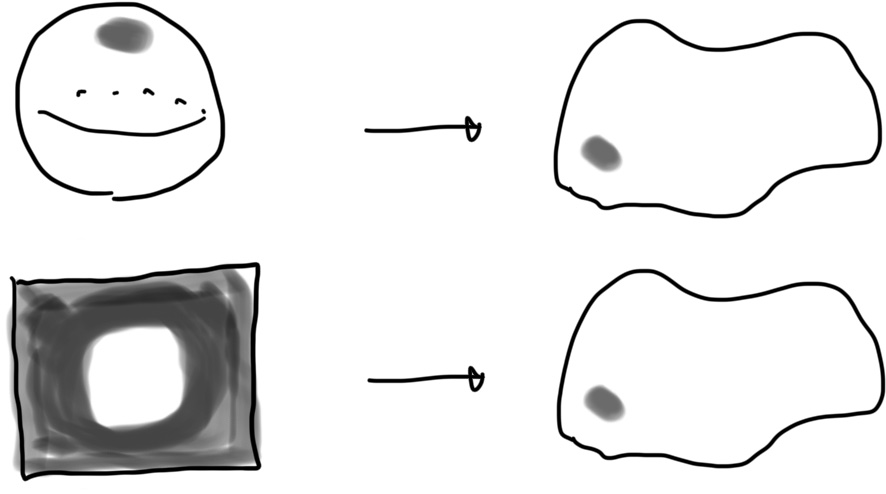
\includegraphics[width=0.5\textwidth]{homotopy}
  \caption{$f\in [S^n,X]_*$ as a map from $[0,1]^n$ to $X$.
  The shaded regions are mapped to the base point $*\in X$.}
  \label{fig:homotopy}
\end{figure}

We can define a group operation on $[S^n,X]_*$ as follows.
Take $f,g\in [S^n,X]_*$.
Regard them as maps $f,g:[0,1]^n\to X$. 
We then define $fg:[0,1]^n \to X$ by \begin{equation}
  (fg)(x_1,\ldots,x_n) = \begin{cases}
    f(2x_1,x_2,\ldots,x_n) & \text{for $x_1\in [0,1/2]$},\\
    g(2x_1-1,x_2,\ldots,x_n) & \text{for $x_1\in [1/2,1]$},
  \end{cases}
\end{equation}
see Fig.~\ref{fig:homotopy-grouplaw}.

\begin{figure}
\[
  \vcenter{\hbox{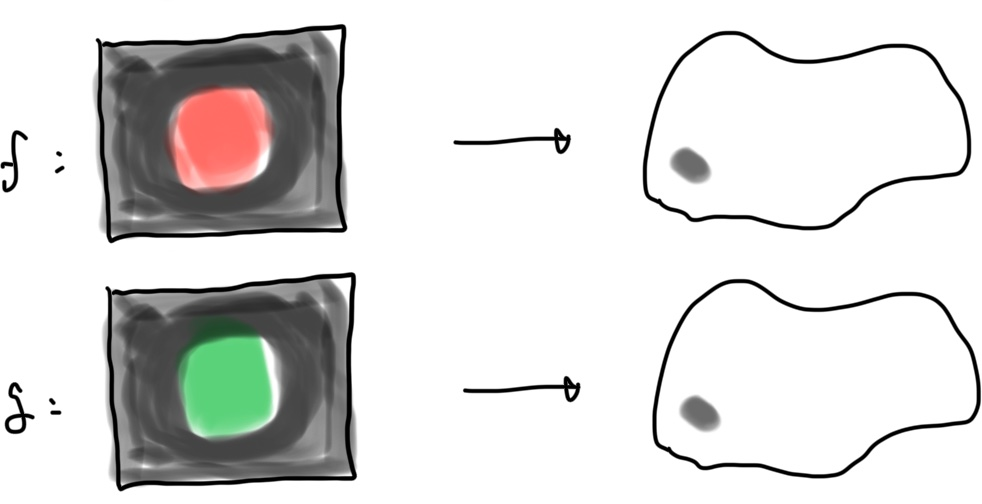
\includegraphics[width=.4\textwidth]{fg.jpg}}}\qquad
  \vcenter{\hbox{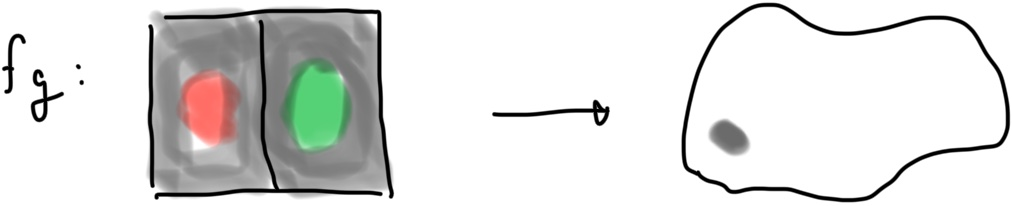
\includegraphics[width=.4\textwidth]{grouplaw.jpg}}}
\]
  \caption{The group operation $fg$ on $[S^n,X]_*$.
  The shaded regions are mapped to the base point $*\in X$.}
  \label{fig:homotopy-grouplaw}
\end{figure}
We also define $f^{-1}$ by \begin{equation}
  f^{-1}(x_1,\ldots,x_n) = 
    f(1-x_1,x_2,\ldots,x_n) 
\end{equation}
As the identity element, we use $e:S^n \to X$ which maps the entire $S^n$ to the base point $*\in X$.

\begin{proposition}
  The set $[S^n,X]_*$ for $n\ge 1$ with the group operation defined above is a group.
\end{proposition}

\begin{definition}
  The group $[S^n,X]_*$ for $n\ge 1$ is called the $n$-th homotopy group of $X$,
  and is denoted by $\pi_n(X)$.
\end{definition}

For $n=1$, $\pi_1(X)$ is also called as the fundamental group of $X$.
It is the group of closed paths from the base point to the base point,
where the group law is obtained by concatenation. 

\begin{example}
$\pi_n(\pt)=0$, where $\pt$ is a single point.
\end{example}

\begin{example}
  $\pi_n(\bR^k)=0$.
\end{example}

\begin{example}
$\pi_1(S^1)=[S^1,S^1]_*=\bZ$. 
\end{example}
This is because $f:S^1\to S^1$ is determined by how many times the image of $f$
winds around $S^1$ when we go around the source $S^1$ once.
This number is called the winding number in physics literature.
Mathematicians call it the \emph{degree} of the map.
See Fig.~\ref{fig:winding} for an illustration.

\begin{figure}[h]
  \centering
  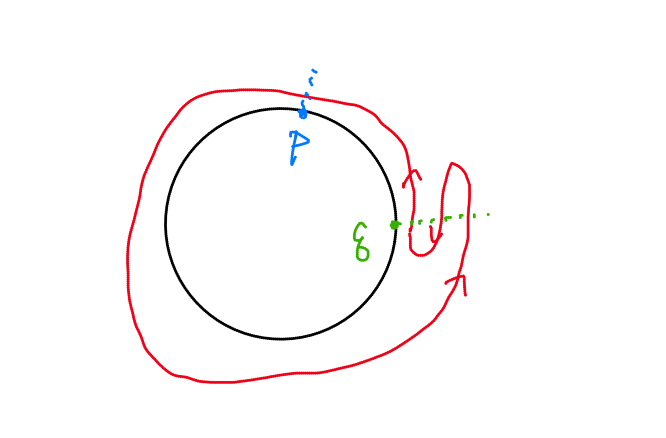
\includegraphics[width=0.3\textwidth]{winding}
  \caption{The winding number of a map $f:S^1\to S^1$.}
  \label{fig:winding}
\end{figure}

As shown there, a way to make this concept more precise is to pick a generic point $p$ in the target $S^1$,
and consider its preimage $f^{-1}(p)$.
This consists in general of a finite number of points in the source $S^1$.
We can count the number of points weighted by the local orientation of $f$ at each point.
This can be shown to be independent of the choice of $p$ in the target $S^1$,
and gives a definition of the winding number.
In Fig.~\ref{fig:winding}, the preimage of $p$ consists of one point, giving $+1$ for the winding number;
the preimage of $q$, in contrast, consists of three points,
with local orientations $+1$, $-1$, $+1$ respectively,
again giving $+1-1+1=+1$ for the winding number.

\begin{example}
  For a genus-$g$ surface $\Sigma_g$, \begin{multline}
  \pi_1(\Sigma_g)= \langle A_1,B_1,A_2,B_2,\ldots,A_g,B_g \mid \\
  A_1 B_1 A_1^{-1} B_1^{-1} A_2 B_2 A_2^{-1} B_2^{-1} \cdots A_g B_g A_g^{-1} B_g^{-1} \rangle.
  \end{multline}
\end{example}
Here $A_i$ and $B_i$ aret the closed paths starting and ending at the base point,
going around the $i$-th hole in two ways, see Fig.~\ref{fig:genus-2}.
The notation on the right hand side, $\langle a,b,\ldots \mid 
\text{relation}_1, \text{relation}_2,\ldots,\rangle$
is called a presentation of a group.

\begin{figure}[h]
  \centering
  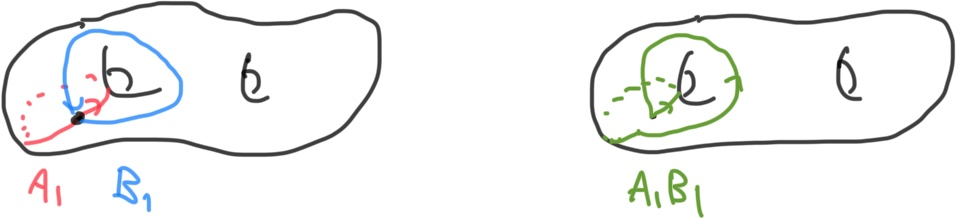
\includegraphics[width=0.6\textwidth]{genus2}
  \caption{Generators of $\pi_1(\Sigma_2)$.}
  \label{fig:genus-2}
\end{figure}

This is an Abelian group when $g=1$, i.e.~for $\Sigma_1=T^2$.
Explicitly, $\pi_1(T^2)=\bZ^2$.
But this is a non-Abelian discrete group for $g\ge 2$.

In contrast, we have:
\begin{proposition}
The group $\pi_n(X)$ is Abelian for $n\ge 2$.
\end{proposition}

For a proof, see Fig.~\ref{fig:commutativity}.
The point is that we can continuously move the nontrivial part of maps $f$ and $g$ across each other,
using the large region in $[0,1]^n$ where $f$ and $g$ are both mapped to the base point.
This is possible only when $n\ge 2$.

\begin{figure}[h]
  \centering
  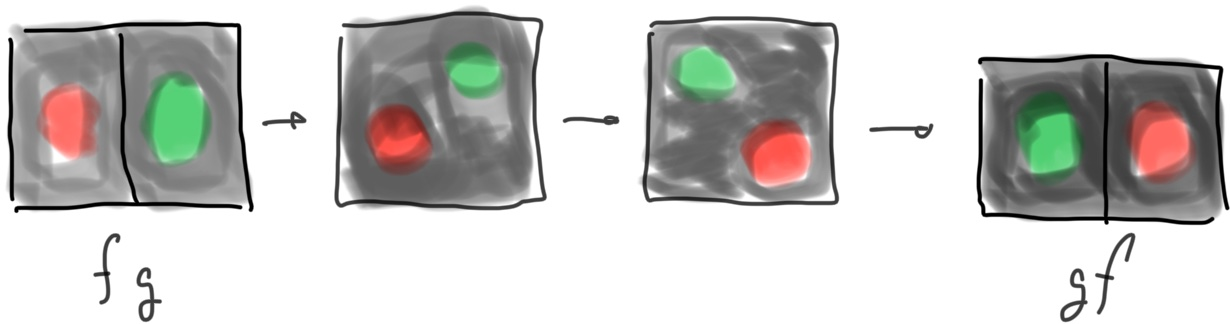
\includegraphics[width=0.6\textwidth]{commutativity}
  \caption{Commutativity of the group operation in $\pi_n(X)$ for $n\ge 2$.}
  \label{fig:commutativity}
\end{figure}

It is also sometimes useful to define the following:

\begin{definition}
We define $\pi_0(X)$ to be $[S^0,X]_*$. This is the set of connected components of $X$.
\end{definition}
Indeed, $S^0=\{*,p\}$  where $*$ is the basepoint.
Then $f:S^0\to X$ is determined by $f(p)\in X$.
We regard $f$ up to homotopy. This means that $f$ is determined by the connected component of $X$ which $f(p)$ is in.

We summarize the considerations so far:
\begin{itemize}
\item $\pi_0(X)$ is a set.
\item $\pi_1(X)$ is a group, known also as the fundamental group of $X$.
\item $\pi_{n\ge 2}(X)$ is an Abelian group.
\end{itemize}

It turns out to be useful to introduce the following notion:
\begin{definition}
  \label{def:n-connected}
A space $X$ is called \emph{connected} if $\pi_0(X)=0$,
and \emph{simply connected} if $\pi_{0,1}(X)=0$.
More generally, a space $X$ is called $n$-connected 
if $\pi_{0,\ldots,n}(X)=0$.
\end{definition}
In particular, $0$-connected means connected
and $1$-connected means simply-connected.

\subsection{Basic properties of homotopy groups}

\begin{definition}
  For a map $f:X\to Y$ and $a:S^n \to X,$ we have a map $f\circ a:S^n\to Y$.
  This determines a map $\pi_n(X)\to \pi_n(Y)$,
  which can be easily seen to be  homomorphism.
\end{definition}

\begin{proposition}
  If two maps $f,g:X\to Y$ are homotopic,
  the corresponding homomorphisms $f_*,g_*:\pi_n(X)\to \pi_n(Y)$ are the same.
\end{proposition}

In particular, if $f:X\to X$ is homotopic to identify,
$f_*:\pi_n(X)\to \pi_n(X)$ is an isomorphism.
This motivates the following definition:

\begin{definition}
  Two spaces $X$ and $Y$ are called homotopy equivalent
  if there are maps $f:X\to Y$ and $g:Y\to X$ such that 
  $f\circ g$ is homotopic to $id_Y$  
  and $g\circ f$ is homotopic to $id_X$.
\end{definition}

Then we have the following:
\begin{proposition}
  If $f: X\to Y$ gives a homotopy equivalence,
  then $f_* \pi_n(X)\to \pi_n(Y)$ is an isomorphism.
\end{proposition}
  
%We are going to define an equivalence relation between spaces
%which is much looser than homeomorphism/diffeomorphism.

When $X$ and $Y$ are homeomorphic, i.e.~if there is a 1:1 continuous map $f:X\to Y$,
taking $g=f^{-1}$ we see that $X$ and $Y$ are homotopy equivalent.
But $X$ and $Y$ being homotopy equivalent is much looser.
\begin{example}
A disk $D^2=\{|x|^2+|y|^2\le 1\}$ is homotopy equivalent to a point.
\end{example}
Indeed, let $f:D^2 \to \{(0,0)\}$ be the obvious map,
and $g:\{(0,0)\}\to D^2$ be the inclusion.
$f\circ g$ is identity.
So we need to show that $g\circ f$ is homotopic to the identity.
For this we just consider $f_s((x,y))= s(x,y)$ for $s\in [0,1]$,
and we are done.
Similarly,
\begin{example}
A disk $D^n$ in any dimension is homotopy equivalent to a point.
\end{example}

So, if we can compute $\pi_n(X)$ and $\pi_n(Y)$ for some $n$ and show $\pi_n(X)\neq \pi_n(Y)$, 
then $X$ and $Y$ are not equivalent under this very loose equivalence relation.
In particular, $X$ and $Y$ are not homeomorphic and not diffeomorphic. 
This is how the homotopy groups $\pi_n(X)$ helps in distinguishing spaces.
But we have not yet learned how to compute homotopy groups.
And this is surprisingly hard!

To get some ideas, let us enumerate some more properties:

\begin{proposition}
  $\pi_n(X\times Y) = \pi_n(X) \times \pi_n(Y)$.
\end{proposition}
This allows the computation of homotopy groups of product manifolds 
to those of the factors.

\begin{proposition}
If $X$ is a manifold, then $\pi_n(X)$ is a finitely generated group.
\end{proposition}
In particular, $\pi_n(X)$ cannot be a continuous group such as $U(N)$.

The structure of finitely generated Abelian groups are well-known:
\begin{fact}
Finitely generated Abelian group $A$ is of the form \begin{equation}
A=\bZ^n \oplus \bZ_{m_1} \oplus \cdots \oplus \bZ_{m_k}.
\label{eq:fin-gen-Abelian}
\end{equation}
\end{fact}

\begin{definition}
In the above decomposition, $\bZ^n$ is called the \emph{free part} of $A$,
and $\bZ_{m_1} \oplus \cdots \oplus \bZ_{m_k}$ is called the \emph{torsion part} of $A$.
\end{definition}

So $\pi_n(X)$ for a manifold $X$ with $n\ge 2$ is always of the form \eqref{eq:fin-gen-Abelian}.

\subsection{Facts on $\pi_n(S^m)$}

Let us have a look at concrete examples of homotopy groups.
As a starter, let us consider the homotopy groups of spheres themselves,
$\pi_n(S^m)=[S^n,S^m]_*$.

\begin{theorem}
$\pi_n(S^m) =0$ if $n<m$.
\end{theorem}
Roughly, a generic map $S^n\to S^m$ with $n<m$ has a point $p\in S^m$ not mapped from $S^n$. 
We can `push' the image of maps from that point to the base point.
So every map is homotopic to the map to the basepoint, see Fig.~\ref{fig:nm}.

\begin{figure}
  \centering
  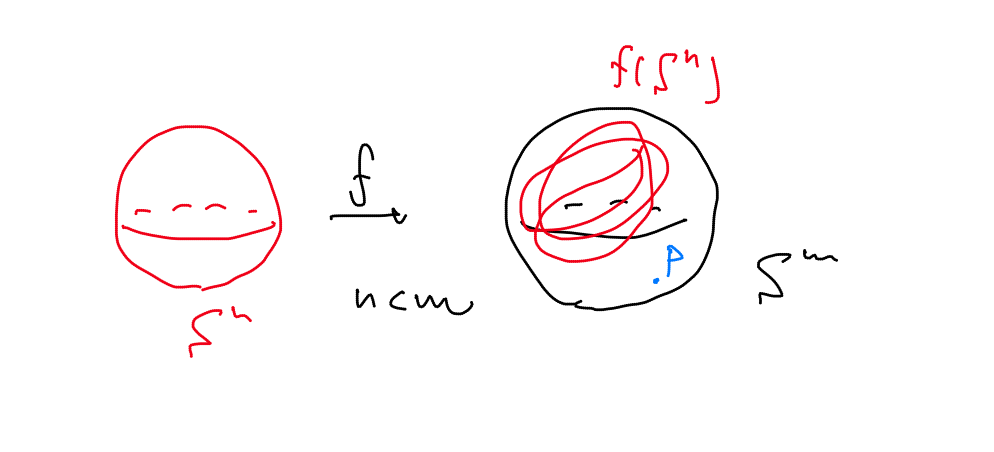
\includegraphics[width=0.6\textwidth]{nm}
  \caption{A generic map $S^n\to S^m$ with $n<m$ has a point $p\in S^m$ not mapped from $S^n$.}
  \label{fig:nm}
\end{figure}


\begin{theorem}
$\pi_n(S^n) =\bZ$.
\end{theorem}
This can be shown by considering 
the higher-dimensional version of the winding number.
For a map $f:S^n\to S^n$, 
the resulting integer is known as its \emph{degree} in mathematics.

A more interesting one is the following:
\begin{theorem}
  $\pi_3(S^2)=\bZ$ and the Hopf fibration $S^3\to S^2$ corresponds 
  to the generator of $\bZ$.
\end{theorem}

%($\nu d\nu$ where  $d\nu$ is the pull back of the volume form)


Given a map $f:S^3\to S^2$, the corresponding integer is obtained as follows.
Pick a generic point $p$ on $S^2$. 
Its inverse image $f^{-1}(p)$ is a collection of circles $C_1,\ldots, C_n$ in $S^3$.
Take another point $q$ on $S^2$.
Its inverse image $f^{-1}(q)$ is another collection of circles $C'_1,\ldots, C'_m$ in $S^3$.
We now consider \begin{equation}
\sum_{i,j} (\text{linking number of $C_i$ and $C'_j$}), \label{eq:Hopf-invariant-crude}
\end{equation}
where the linking number of two circles is defined in the standard way.\footnote{This appears in the integrated form of the equation of electromagnetism.
Namely, if a current $I$ flows in a loop $C$,
then the integral of the magnetic field around $C'$ 
is proportional to the linking number of $C$ and $C'$.}
One can show that this is independent under continuous deformations of $f$.
This is one definition of the Hopf invariant of $f$.
See Fig.~\ref{fig:hopf-invariant} for an illustration of the definition.

\begin{figure}
  \centering
  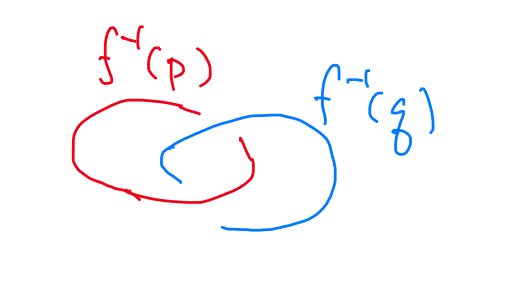
\includegraphics[width=0.4\textwidth]{hopf}
  \caption{A definition of the Hopf invariant of a map $f:S^3\to S^2$  is 
  given by considering the linking number of the inverse images of two points in $S^2$.}
  \label{fig:hopf-invariant}
\end{figure}

We drew the actual fibers of the Hopf fibration $S^1\to S^3\to S^2$ in Fig.~\ref{fig:hopf-fibers}.
By inspection, we see that two fibers have the linking number $1$. 
Therefore, the Hopf fibration $S^3\to S^2$ has the Hopf invariant $1$.

We can similarly define linking numbers of two $S^{n-1}$'s within $S^{2n-1}$,
where the previous case corresponds to $n=2$.
Then, for a map $f: S^{2n-1}\to S^{n}$,
the inverse image of a generic point in $S^n$ is a $(n-1)$-dimensional space,
and then we can define a higher-dimensional Hopf invariant of $f$ as in \eqref{eq:Hopf-invariant-crude}.
It is relatively easy to construct a map $S^{2n-1}\to S^n$ with Hopf invariant 2 for general $n$, and therefore
\begin{theorem}
  $\pi_{2n-1}(S^n)$ contains a  $\bZ$ summand.
\end{theorem}

Also, by an explicit computation we can show  that \begin{proposition}
The Hopf fibrations $S^1\to S^1$, $S^3\to S^2$, $S^7\to S^4$,
all have Hopf invariant one.
\end{proposition}
and in fact 
\begin{theorem}
There is a map $f:S^{2n-1}\to S^n$ with Hopf invariant one
only when $n=1,2,4$.
\end{theorem}
This is a deep result in algebraic topology, known as the Hopf invariant one problem,
and the efforts to solve this question inspired many developments in the field.


Another interesting fact is that 

\begin{theorem}
  The only free part of $\pi_n(S^m)$ is $\pi_n(S^n)\simeq \bZ$
  and the single $\bZ$ summand of $\pi_{2n-1}(S^n)$ discussed above.
  Otherwise the homotopy groups of spheres are all torsion.
\end{theorem}
  

With these basic properties covered,
let us have a look at the homotopy groups of spheres $\pi_{n+k}(S^n)$ 
for small $n$ and $k$, which are tabulated in Table~\ref{tab:pi_nS^m}.
The data are taken from 岩波数学辞典 \cite[付録, 公式 7, V]{Jiten},
which also has an English translation \cite{EDM}.

\begin{table}[h]
  \[
\begin{array}{c|cccccccccccccccccc}
  k & 0 & 1 & 2 & 3 & 4 & 5 & 6 & 7 & 8 & 9  \\
   \hline
  S^1 & \textcolor{red}{\bZ} & 0 & 0 & 0 & 0 & 0 & 0 & 0 & 0 & 0 \\
  S^2 & \cellcolor{lg} \textcolor{red}{\bZ} & \textcolor{blue}{\bZ} & \bZ_2 & \bZ_2 & \bZ_{12} & \bZ_2 & \bZ_2 & \bZ_3 & \bZ_{15} & \bZ_2  \\
  S^3 & \cellcolor{lg} \textcolor{red}{\bZ} & \cellcolor{lg} \bZ_2 & \bZ_2 & \bZ_{12} & \bZ_2 & \bZ_2 & \bZ_3 & \bZ_{15} & \bZ_2 & (\bZ_2)^2  \\
  S^4 &\cellcolor{lg}  \textcolor{red}{\bZ} & \cellcolor{lg} \bZ_2 & \cellcolor{lg} \bZ_2 & \textcolor{blue}{\bZ} \times \bZ_{12} & (\bZ_2)^2 & (\bZ_2)^2 & \bZ_{24} \times \bZ_3 & \bZ_{15} & \bZ_2  & (\bZ_2)^3\\
  S^5 & \cellcolor{lg} \textcolor{red}{\bZ} & \cellcolor{lg} \bZ_2 & \cellcolor{lg} \bZ_2 & \cellcolor{lg} \bZ_{24} & \bZ_2 & \bZ_2 & \bZ_2 & \bZ_{30} & \bZ_2 & (\bZ_2)^3  \\
  S^6 & \cellcolor{lg} \textcolor{red}{\bZ} & \cellcolor{lg} \bZ_2 & \cellcolor{lg} \bZ_2 & \cellcolor{lg} \bZ_{24} & \cellcolor{lg} 0 & \textcolor{blue}{\bZ} & \bZ_2 & \bZ_{60} & \bZ_{24}\times \bZ_2 & (\bZ_2)^3\\
  S^7 &\cellcolor{lg}  \textcolor{red}{\bZ} & \cellcolor{lg} \bZ_2 & \cellcolor{lg} \bZ_2 & \cellcolor{lg}\bZ_{24} & \cellcolor{lg} 0 &\cellcolor{lg}  0 & \bZ_2 & \bZ_{120} & (\bZ_2)^3 & (\bZ_2)^4 \\
  S^8 & \cellcolor{lg} \textcolor{red}{\bZ} & \cellcolor{lg} \bZ_2 & \cellcolor{lg} \bZ_2 & \cellcolor{lg} \bZ_{24} & \cellcolor{lg} 0 & \cellcolor{lg} 0 & \cellcolor{lg} \bZ_2 & \textcolor{blue}{\bZ}\times \bZ_{120} & (\bZ_2)^4 & (\bZ_2)^5 \\
  S^9 &\cellcolor{lg}  \textcolor{red}{\bZ} & \cellcolor{lg} \bZ_2 & \cellcolor{lg} \bZ_2 & \cellcolor{lg} \bZ_{24} & \cellcolor{lg} 0 & \cellcolor{lg} 0 & \cellcolor{lg} \bZ_2 & \cellcolor{lg} \bZ_{240} & (\bZ_2)^3 & (\bZ_2)^4 \\
  S^{10} &\cellcolor{lg}  \textcolor{red}{\bZ} & \cellcolor{lg} \bZ_2 & \cellcolor{lg} \bZ_2 & \cellcolor{lg} \bZ_{24} & \cellcolor{lg} 0 & \cellcolor{lg} 0 & \cellcolor{lg} \bZ_2 & \cellcolor{lg} \bZ_{240} & \cellcolor{lg} (\bZ_2)^2 & \textcolor{blue}{\bZ}\times (\bZ_2)^3 \\
  S^{11} &\cellcolor{lg}  \textcolor{red}{\bZ} & \cellcolor{lg} \bZ_2 & \cellcolor{lg} \bZ_2 & \cellcolor{lg} \bZ_{24} & \cellcolor{lg} 0 & \cellcolor{lg} 0 & \cellcolor{lg} \bZ_2 & \cellcolor{lg} \bZ_{240} & \cellcolor{lg} (\bZ_2)^2 & \cellcolor{lg} (\bZ_2)^3 \\
  S^{12} &\cellcolor{lg}  \textcolor{red}{\bZ} & \cellcolor{lg} \bZ_2 & \cellcolor{lg} \bZ_2 & \cellcolor{lg} \bZ_{24} & \cellcolor{lg} 0 & \cellcolor{lg} 0 & \cellcolor{lg} \bZ_2 & \cellcolor{lg} \bZ_{240} & \cellcolor{lg} (\bZ_2)^2 & \cellcolor{lg} (\bZ_2)^3 \\
\end{array}
\]
\caption{Table of $\pi_{n+k}(S^n)$ \label{tab:pi_nS^m}}
\end{table}

Here we showed $\pi_d(S^d)\simeq \bZ$ in red,
and the $\bZ$ summand of $\pi_{2d-1}(S^d)$ in blue.

We clearly see more patterns in the table. 
This comes from the following general fact.
Let us start with a definition.
\begin{definition}
Given a pointed space $(X,*)$,
we define the reduced suspension $\Sigma X$ of $X$ as \begin{equation}
  \Sigma X = \frac{ X \times [0,1]}{
    X \times \{0,1\} \cup \{*\} \times [0,1]
  }. 
\end{equation}
\end{definition}

See Fig.~\ref{fig:suspension} for an illustration.
\begin{figure}
  \centering
  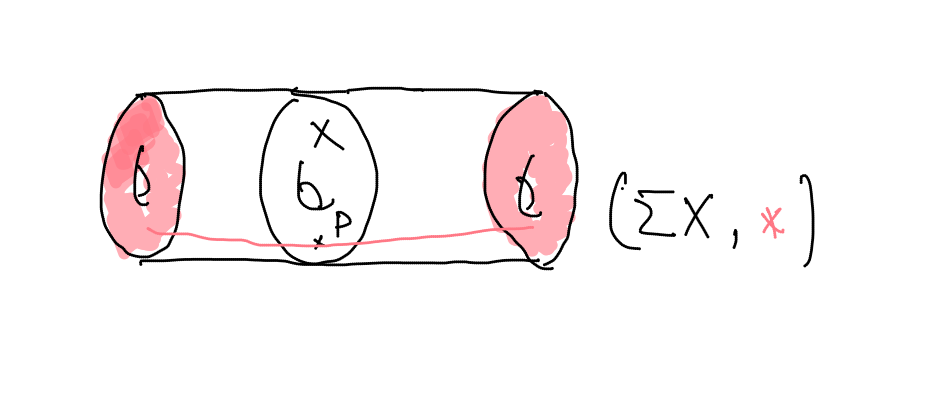
\includegraphics[width=0.5\textwidth]{suspension}
  \caption{The reduced suspension $\Sigma X$ of a space $X$.
  In the figure, we collapse all the points colored in red to a single point,
  which we take to be the basepoint.}
  \label{fig:suspension}
\end{figure}

\begin{proposition}
  $\Sigma S^n \simeq S^{n+1}$.
\end{proposition}

\begin{definition}
Given $f:X\to Y$, we define $\Sigma f:\Sigma X\to \Sigma Y$ by \begin{equation}
  (\Sigma f)([x,t]) = ([f(x),t]),
\end{equation}
where we denoted a point in $\Sigma X$ by $[x,t]$ for $x\in X$ and $t\in[0,1]$.
This determines a map \begin{equation}
[X,Y]_*\to [\Sigma X,\Sigma Y]_*.
\end{equation}
\end{definition}

In particular, when applied to $X=S^n$ and $\Sigma X=S^{n+1}$, we have 
\begin{proposition}
$\pi_n(Y)\to \pi_{n+1}(\Sigma Y)$ is a homomorphism of groups.
\end{proposition}
Furthermore, there is the Freudenthal suspension theorem:
\begin{theorem}
Suppose $Y$ is $(n-1)$-connected, i.e.~$\pi_{i<n}(Y)=0$.
Then the suspension homomorphism $\pi_k(Y)\to \pi_{k+1}(\Sigma Y)$ is an isomorphism for $k< 2n-1$ and a surjection for $k=2n-1$.
\end{theorem}
More explicitly, $\pi_{k\ge n}(\Sigma Y)=0$,
$\pi_{k}(Y)=\pi_{k+1}(\Sigma Y)$ for $k=0,1,\ldots,2n-1$,
and $\pi_{2n}(Y)\to \pi_{2n+1}(\Sigma Y)$ is surjective.

As $S^n$ is clearly $(n-1)$-connected, we see in particular 
\begin{proposition}
  $\pi_{n+k}(S^n)\to \pi_{(n+1)+k}(S^{n+1})$ 
  is an isomorphism for $k<n-1$ and a surjection for $k=n-1$.
\end{proposition}
This explains the grayed area in Table~\ref{tab:pi_nS^m}.

The homotopy groups of spheres in the grayed area 
are known as the stable homotopy groups of spheres.
More precisely, mathematicians define the following:
\begin{definition}
  We call \begin{equation}
   \pi^\text{st}_k := \lim_{n\to\infty} \pi_{n+k}(S^n)
  \end{equation}
as the $k$-th stable homotopy group of spheres,
or simply the $k$-th stem.
\end{definition}

In contrast, the homotopy groups in the ungrayed area
are known as unstable groups.
The stable homotopy groups of spheres are much easier to compute than the unstable groups.
Still, the stable homotopy groups are not quite understood.
Indeed, computing them is a major goal in algebraic topology;
currently it is known up to $k\ge 83$ \cite{Isaksen}.

In this field, there is a famous principle known as the 
`Mahowald uncertainty principle' \cite[Sec.~3]{IsaksenICM},
which says 
that there is no single method 
which allows us to compute all the stable homotopy groups of spheres!
%\footnote

Before moving on to the next section,
let us discuss a particular homotopy group of spheres in the stable range
which is relevant to the Standard Model of particle physics:
\begin{example}
  $\pi_4(S^3)=\bZ_2$.
\end{example}
Using the Freudenthal suspension theorem,
we know that its generator $S^4\to S^3$ is the suspension $\Sigma p$
of the Hopf fibration $p:S^3\to S^2$.
But it is difficult to see that this map $\Sigma p$ 
generates a $\bZ_2$, and that there is no other generator.
  
The way it appears in four-dimensional physics is the following.
The weak force is described by a $SU(2)$ gauge theory,
and therefore we have an $SU(2)$ principal bundle over our spacetime.
Take a patch $\bR^4$ of the spacetime.
Then we can consider a gauge transformation \begin{equation}
  g:\bR^4\to SU(2).
\end{equation}
Let us say we don't perform any gauge transformation in the far region.
Then we essentially have a map \begin{equation}
g: S^4\to SU(2) \simeq S^3. \label{eq:su2gaugetr}
\end{equation}
Now, we have various fermions in our world.
Those charged under the weak force 
are always in the doublet representation of $SU(2)$.
A single doublet is described by a section of $\underline{\mathbf{2}}\otimes S\to M$ 
in the notation of Sec.~\ref{sec:SM};
$\underline{V}\to M$ 
is the associated vector bundle
for a representation $\rho: G \curvearrowright V$
and a principal $G$-bundle $P\to M$,
and $S\to M$ is the spin bundle.

Now, the partition function $Z_\text{single doublet}$ of a fermion in a singlet doublet representation 
of $SU(2)$ 
is known to behave under 
a gauge transformation \eqref{eq:su2gaugetr} as \begin{equation}
  Z_\text{single doublet} \to (-1)^s Z_\text{single doublet}.\label{eq:Witten-anomaly}
\end{equation}
where $s=[g] \in \pi_4(S^3) \simeq \bZ_2 \simeq \{0,1\}$;
this was found originally in \cite{Witten:1982fp}.
This means that an $SU(2)$ gauge theory with a single doublet is inconsistent, for example.

Now, in a single generation \eqref{eq:generation},
there are $3+1=4$ doublets of $SU(2)$.
Therefore, the sign \eqref{eq:Witten-anomaly} always becomes $(-1)^{4s}=+1$,
making the theory consistent.
This for example means that you cannot just change the number of colors $SU(3)$ to $SU(4)$, 
keeping everything else in the Standard Model fixed.


\subsection{Long exact sequence of homotopy groups of fiber bundles}
\subsubsection{Statement}
Computing homotopy groups is hard. 
One useful technique is the long exact sequence of homotopy groups
associated to fiber bundles $F\to E\to B$.
This relates the homotopy groups  $\pi_*(F)$, $\pi_*(E)$, and $\pi_*(B)$.
This often allows us to determine one if we know the other two.
We start from the following definition:

\begin{definition}
  A sequence of groups and homomorphisms between them, \begin{equation}
  \cdots 
  \stackrel{f_{i-2}}{\longrightarrow} G_{i-1} 
  \stackrel{f_{i-1}}{\longrightarrow} G_{i}
  \stackrel{f_{i}}{\longrightarrow} G_{i+1}
  \stackrel{f_{i+1}}{\longrightarrow} \cdots
  \end{equation}
is called an exact sequence of groups if it is exact at each group, i.e.~
$f_{i-1}\circ f_i=0$ and furthermore 
\begin{equation}
 \Im f_{i}  = \Ker f_{i+1} \subset G_i \label{eq:exactness}
\end{equation}
for all $i$.
\end{definition}

\begin{definition}
  A short exact sequence of groups is an exact sequence of groups of the following form: \begin{equation}
  1 \to A \to B \to C \to 1.
  \end{equation}
  In this case $B$ is called the extension of $C$ by $A$.
\end{definition}
Note that for Abelian groups we often use the notation $0$ instead of $1$
to denote a trivial group.

Given $A$ and $C$, $B$ is not uniquely determined.
For example, assuming all groups involved to be Abelian,
consider the short exact sequence \begin{equation}
  0 \to \bZ_2 \to A \to \bZ_2 \to 0.
\end{equation}  
Then $A$ can be $\bZ_2\times \bZ_2$ or $\bZ_4$.
In the latter case, the homomorphisms are given by \begin{equation}
0 \to \{0,1\} \xrightarrow{\times 2} \{0,1,2,3\} \xrightarrow{\mod 2} \{0,1\} \to 0.
\end{equation}

But there are cases when the extension is unique. 
The most obvious but still useful cases are:
\begin{example}
An exact sequence $1\to A\to B\to 1$ means that $A\simeq B$.
\end{example}

\begin{proposition}
  An exact sequence of groups\begin{equation}
    \cdots 
    \stackrel{f_{i-2}}{\longrightarrow} G_{i-1} 
    \stackrel{f_{i-1}}{\longrightarrow} G_{i}
    \stackrel{f_{i}}{\longrightarrow} G_{i+1}
    \stackrel{f_{i+1}}{\longrightarrow} \cdots
  \end{equation}
  gives rise to short exact sequences of groups \begin{equation}
    0 \to G_{i-1}/\Ker f_{i-1} \to G_i \to \Im f_{i} \to 0.
  \end{equation}
\end{proposition}

This means that, given a long exact sequence of groups,
we have a lot of information to determine the groups involved.
Let us come back to algebraic topology.
\begin{theorem}
  \label{thm:long-exact-seq-homotopy}
  Given a fiber bundle \begin{equation}
    F\stackrel{\iota}{\longrightarrow} E\stackrel{p}{\longrightarrow} B,
  \end{equation}
  we have the following long exact sequence of homotopy groups: 
  \begin{equation}\begin{array}{cccccccc}
    \cdots 
      & \stackrel{\partial}{\longrightarrow} & \pi_{n+1}(F)  
      & \stackrel{\iota_*}{\longrightarrow} & \pi_{n+1}(E)
      & \stackrel{p_*}{\longrightarrow} & \pi_{n+1}(B)  \\
      & \stackrel{\partial}{\longrightarrow} & \pi_{n}(F)  
      & \stackrel{\iota_*}{\longrightarrow} & \pi_{n}(E)
      & \stackrel{p_*}{\longrightarrow} & \pi_{n}(B)  \\
      & \stackrel{\partial}{\longrightarrow} & \cdots & &&& \cdots \\
      & \stackrel{\partial}{\longrightarrow} & \pi_{1}(F)  
      & \stackrel{\iota_*}{\longrightarrow} & \pi_{1}(E)
      & \stackrel{p_*}{\longrightarrow} & \pi_{1}(B) \\
      & \stackrel{\partial}{\longrightarrow} & \pi_{0}(F)  
      & \stackrel{\iota_*}{\longrightarrow} & \pi_{0}(E)
      & \stackrel{p_*}{\longrightarrow} & \pi_{0}(B),
      \end{array}\end{equation}
      where the last three objects are not really groups but sets,
      but the condition \eqref{eq:exactness} still holds,
      and the map $\partial$ is constructed below in Definition~\ref{def:connecting-map-homotopy}.  
\end{theorem}


\subsubsection{Use cases}
Let us have a look at some of the basic use cases. 
This shows that you can use a theorem without understanding its proof,
and without even understanding the construction of the important map $\partial$
in the statement!
This is the mindset ``math as a set of mobile apps'' I am advocating.

Consider the fiber bundle $\bZ\to \bR \to S^1$.
As $\pi_n(\bR^k)=0$, the long exact sequence simply gives
\begin{equation}
0=\pi_n(\bR)\to \pi_n(S^1)\to \pi_{n-1}(\bZ)\to \pi_{n-1}(\bR)=0
\end{equation} meaning that \begin{equation}
  \pi_n(S^1)=\pi_{n-1}(\bZ).
\end{equation} As $\pi_0(\bZ)=\bZ$ and $\pi_{n\ge 1}(\bZ)=0$,
we conclude that \begin{equation}
  \pi_n(S^1)=\begin{cases}
    \bZ & n=1, \\
    0 & n\neq 1.
  \end{cases}
\end{equation}

Suppose $\Gamma$ acts on $S^n$ freely, with $n\ge 2$. 
We have the fiber bundle $\Gamma\to S^n\to S^n/\Gamma$.
Then we have the long exact sequence, a part of which is \begin{equation}
  \pi_1(S^n) \to \pi_1(S^n/\Gamma)\to \pi_0(\Gamma) \to \pi_0(S^n)
\end{equation} which is \begin{equation}
   0 \to \pi_1(S^n/\Gamma) \to \Gamma\to 0
\end{equation} meaning that $\pi_1(S^n/\Gamma)=\Gamma$.
Recall $\RP^n=S^n/\bZ_2$. Therefore we have \begin{equation}
  \pi_1(\RP^n)=\bZ_2.
\end{equation}
Recall further that $SO(3)=\bZ_2$. Then we have \begin{equation}
  \pi_1(SO(3))=\bZ_2.
\end{equation}

Next, let us apply the long exact sequence of homotopy groups to the Hopf fibration $S^1\to S^3\to S^2$.
We learned above that $\pi_k(S^1)=0$ when $k>1$.
Therefore the long exact sequences gives \begin{equation}
  0=\pi_{k}(S^1)\to \pi_{k}(S^3)\to \pi_k(S^2)\to \pi_{k-1}(S^1)=0
\end{equation} when $k\ge 3$, meaning that \begin{equation}
  \pi_k(S^3)=\pi_k(S^2)
\end{equation} again with $k\ge 3$. 
This in particular shows that $\pi_3(S^2)=\bZ$, the basic fact we already mentioned,
and also explains the pattern in Table~\ref{tab:pi_nS^m}
in the two columns for $S^2$ and $S^3$.

As another example, consider the computation of $\pi_1(SO(n))$.
We just saw above that $\pi_1(SO(3))=\bZ_2$.
We learned in Proposition \ref{prop:SO/SO} that there is a fiber bundle
\begin{equation}
SO(n-1)\to SO(n)\to S^{n-1}.
\end{equation} Then the long exact sequence gives
\begin{equation}
  \pi_2(S^{n-1})\to \pi_1(SO(n-1))\to \pi_1(SO(n))\to \pi_1(S^{n-1}).
\end{equation}
For $n>  3$ we have $\pi_{2}(S^{n-1})=\pi_1(S^{n-1})=0$, and therefore $\pi_1(SO(n-1))=\pi_1(SO(n))$.
Inductively, we have found 
\begin{example}
  \label{ex:pi1SOn}
$\pi_1(SO(n))=\bZ_2$ for $n\ge 3$.
\end{example}


A different part of the same long exact sequnece for $n=3$ gives \begin{equation}
  \underbrace{\pi_2(SO(2))}_{=0}
  \to \pi_2(SO(3)) 
  \to \underbrace{\pi_2(S^2)}_{\bZ}
  \stackrel{\partial}{\longrightarrow}  \underbrace{\pi_1(SO(2))}_{\bZ} \to \underbrace{\pi_1(SO(3))}=\bZ_2  \pi_1(S^2)=0.
\end{equation}
This forces $\partial:\bZ\to \bZ$ to be a multiplication by $2$,
which tne means that $\pi_2(SO(3))=0$.

As a final example, consider the computation of $\pi_4(Sp(n))$.
We learned in Proposition \ref{prop:Sp/Sp} that there is a fiber bundle
\begin{equation}
  Sp(n-1)\to Sp(n)\to S^{4n-1}.
\end{equation} Then the long exact sequence gives
\begin{equation}
  \pi_5(S^{4n-1})\to \pi_4(Sp(n-1))\to \pi_4(Sp(n))\to \pi_4(S^{4n-1}).
\end{equation} For $n\ge 2$, $4n-1\ge 7$, and therefore 
\begin{equation}
  0\to \pi_4(Sp(n-1))\to \pi_4(Sp(n))\to 0,
\end{equation} i.e.~$\pi_4(Sp(n-1))=\pi_4(Sp(n))$.
As $\pi_4(Sp(1))=\bZ_2$, we inductively find that 
\begin{example}
  $\pi_4(Sp(n))=\bZ_2$.  
\end{example}
This suggests the existence of the mod-2 $SU(2)=Sp(1)$ anomaly of Witten 
carries on to higher $Sp(n)$ gauge theories,
and it indeed turns out to be the case.

\subsubsection{Idea of the proof}
The idea of the proof of this important theorem is as follows.
Consider first the part \begin{equation}
\pi_{n}(F) \stackrel{\iota_*}{\longrightarrow} \pi_{n}(E) \stackrel{p_*}{\longrightarrow} \pi_{n}(B).
\end{equation}
That $p_*\circ \iota_*=0$ is clear.
But not only that, we need to show that $\Im \iota_* = \Ker p_*$,
So, assume that $f:S^n\to E$ is such that $F=p\circ f: S^n\to B$ is homotopic to a trivial map.
So there is a deformation $F_s$ for $s\in [0,1]$ such that $F_0=F$ and $F_1$ is the constant map.
At each step $F_s$, we can find $f_s:S^n \to E$ such that $p\circ f_s=F_s$.
As $p\circ f_0=F_0$ is a constant map to the base, $f_0$ is actually a map to a fiber, done.

Next, consider the part \begin{equation}
  \pi_{n+1}(B)\stackrel{\partial}{\longrightarrow}\pi_{n}(F) \stackrel{\iota_*}{\longrightarrow} \pi_{n}(E).
\end{equation}
For this we need to define the map $\partial$ to start with.
\begin{figure}[h]
  \centering
  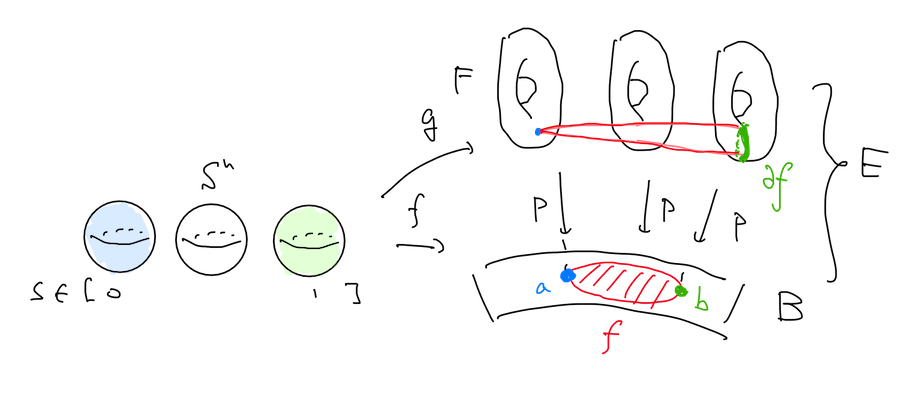
\includegraphics[width=0.8\textwidth]{connecting.png}
  \caption{The connecting map $\partial$}
  \label{fig:connecting}
\end{figure}
\begin{definition}
  \label{def:connecting-map-homotopy}
  $\partial:\pi_{n+1}(B)\to \pi_{n}(F)$ is defined as follows.
  Given a map $f:S^{n+1}\to B$, we regard it instead as a parameterized map
  \begin{equation}
  f: S^n\times [0,1] \to B
  \end{equation} such that \begin{equation}
    f(-,0):S^n\to B,\qquad
    f(-,1):S^n\to B
  \end{equation}
  are constant maps to points $a,b\in B$, respectively.
  We now consider the continuous map \begin{equation}
    \tilde f:S^n\times [0,1]\to E
  \end{equation}
  such that $p\circ \tilde f=f$ and that \begin{equation}
    \tilde f(-,0): S^n\to E
  \end{equation} is a constant map to the basepoint $*\in E$ above $a\in B$.
  Now, the image of  \begin{equation}
    \tilde f(-,1): S^n\to E
  \end{equation} contained in the fiber $F$ above $b\in B$,
  so we can define \begin{equation}
    \partial [f] := [\tilde f(-,1)]\in \pi_n(F).
  \end{equation}
\end{definition}
See Fig~\ref{fig:connecting} for an illustration.
With this definition, the property $\Im \partial = \Ker \iota_*$ is fairly tautological.

Finally, consider the part \begin{equation}
  \pi_{n+1}(E) \stackrel{p_*}{\longrightarrow} \pi_{n+1}(B) \stackrel{\partial}{\longrightarrow} \pi_{n}(F).
\end{equation}
Again, the property $\Im p_* = \Ker \partial$ is fairly tautological.

To get a better idea of the connecting map, it is instructive 
to compute the process explicitly in the case of the Hopf fibration.
For example, consider the following step: \begin{equation}
0= \pi_2(S^3) \to \pi_2(S^2) \stackrel{\partial}{\longrightarrow} \pi_1(S^1) \to \pi_1(S^3)=0.
\end{equation}
Consider the identity map $f:S^2\to S^2$ and let us compute $\partial f$.
Let us use the polar coordinate $(\sin\theta\cos\phi,\sin\theta\sin\phi,\cos\theta)$ for $S^2$.
Then we can regard $\theta\in [0,\pi]$ as $s\in[0,1]$ used in the definition above, so $f(\phi,\theta)=(\phi,\theta)$.

Now, recall the following description \eqref{eq:Hopf-explicit} of the Hopf map $S^3\to S^2$:\begin{equation}
  (\cos(\theta/2)  e^{i \psi},
  \sin(\theta/2) e^{i(\phi+\psi)} )
  \mapsto  (\sin\theta\cos\phi,\sin\theta\sin\phi,\cos\theta).
\end{equation}
Then we can take \begin{equation}
g(\phi,\theta) := (\cos(\theta/2),\sin(\theta/2)e^{i\phi}).
\end{equation}
We indeed see that \begin{equation}
(\partial f)(\phi):= g(\phi,\pi) = (0,e^{i\phi})
\end{equation} which indeed wraps once around the fiber over $(0,0,1)$.


\subsection{Homotopy groups of Lie groups}

To use the long exact sequence of homotopy groups,
we need to know some homotopy groups to start with.
We already gave a table of $\pi_n(S^m)$ for some values of $n,m$.
Here we discuss homotopy groups of Lie groups.


Let us start with $U(1)$. As $U(1)=S^1$, we already know $\pi_n(U(1))$.

Let us then discuss non-Abelian Lie groups $G$.
For groups, $\pi_0(G)$, the set of connected components, itself is a group.
For example, $O(n)$ has two components,
the one with $\det=+1$ and another with $\det=-1$.
Then $\pi_0(O(n))=\bZ_2$. 
For the rest of this subsection, we only consider connected Lie groups,
for which $\pi_0(G)=1$.

Let us next consider $\pi_1(G)$. 
\begin{fact}
$\Gamma$ is always known to be an Abelian group.
Furthermore, it is known that there always is a group $\tilde G$ with $\pi_1(\tilde G)=0$
together with a subgroup $\Gamma \subset \tilde G$ such that \begin{equation}
G=\tilde G/\Gamma.
\end{equation}
Such $\tilde G$ is known as the universal cover of $G$.
\end{fact}
Let us check that $\pi_1(\tilde G/\Gamma)=\Gamma$.
For this we consider the long exact sequence of homotopy groups associated to 
the fiber bundle $\Gamma\to \tilde G\to G$, which is \begin{equation}
\pi_1(\tilde G)\to \pi_1(G)\to \pi_0(\Gamma)\to \pi_0(\tilde G).
\end{equation}
As $\pi_1(\tilde G)=\pi_0(\tilde G)=0$, we see $\pi_1(G)\simeq \pi_0(\Gamma)\simeq \Gamma$.

The case we typically counter is $G=SO(n)$, for which $\pi_1(SO(n))=\bZ_2$ for $n\ge 3$, as we already saw in Example~\ref{ex:pi1SOn}.
The corresponding universal cover is the Spin group $Spin(n)$;
so we have \begin{equation}
\bZ_2 \to Spin(n)\to SO(n).
\end{equation}

Consider compact Lie groups $G$ such that 
it is connected (i.e.~$\pi_0(G)=0$)
and simply-connected (i.e.~$\pi_1(G)=0$).
It is known that such groups are always a product of copies of
$\bR$ and \begin{equation}
SU(n\ge 2),\quad
Spin(n\ge 6),\quad
Sp(n\ge 2),\quad
F_4,\quad
G_2,\quad
E_6,\quad
E_7,\quad
E_8.
\label{eq:list-simple-Lie}
\end{equation}
$Spin(3)=SU(2)$, $Spin(4)=SU(2)^2$, $Spin(5)=Sp(2)$, $Spin(6)=SU(4)$
 and $Sp(1)=SU(2)$ 
were excluded from the list, as they are redundant.

The groups in \eqref{eq:list-simple-Lie} are called compact 
simple simply-connected Lie groups.

\begin{fact}
$\pi_2(G)=0$ and $\pi_3(G)=\bZ$ for groups $G$ in \eqref{eq:list-simple-Lie}.
\end{fact}

\begin{fact}
$\pi_4(G)$ for groups $G$ in \eqref{eq:list-simple-Lie} are 
either $\bZ_2$ for $G=Sp(n)$ or $0$ otherwise.
\end{fact}


We tabulate in Table~\ref{tab:pi_nG}
the homotopy groups of simply connected Lie groups $\pi_{n}(G)$ 
for  $3\le n\le 11$.
The data are taken from \cite[付録, 公式 7, VII]{Jiten}.
(The same set of tables should also be contained in the English translation \cite{EDM}.)

\begin{table}[ht]
  \[
  \begin{array}{c|cccccccccccccccc}
  G~\setminus~d&2&3&4&5&6&7&8&9&10&11 \\
  \hline
  \hline
  \Sp(1) &\cellcolor{lg}0&\cellcolor{lg} \bZ&\cellcolor{lg} \BZ_2 &\cellcolor{lg}\BZ_2 & \BZ_{12} &\BZ_{2} &\BZ_{2} &\BZ_{3} & \bZ_{15} &\bZ_2\\
  \Sp(2) &\cellcolor{lg}0&\cellcolor{lg}\bZ& \cellcolor{lg} \BZ_2 &\cellcolor{lg}\BZ_2 &\cellcolor{lg} 0 &\cellcolor{lg}\BZ_{} &0 &\cellcolor{lg}0 & \bZ_{120} &\bZ_2\\
  \Sp(3) &\cellcolor{lg}0&\cellcolor{lg} \bZ&\cellcolor{lg} \BZ_2 &\cellcolor{lg}\BZ_2 &\cellcolor{lg} 0 &\cellcolor{lg}\BZ_{} &\cellcolor{lg}0 &\cellcolor{lg}0 &\cellcolor{lg} 0 &\cellcolor{lg} \bZ\\
  \hline
  \SU(3) &\cellcolor{lg}0&\cellcolor{lg} \bZ&\cellcolor{lg}0 &\cellcolor{lg}\BZ &\BZ_{6} &0 &\BZ_{12} &\BZ_{3} & \bZ_{30} & \bZ_4 \\
  \SU(4) &\cellcolor{lg}0&\cellcolor{lg}\bZ&\cellcolor{lg}0 &\cellcolor{lg}\BZ &\cellcolor{lg}0 &\cellcolor{lg}\BZ &\BZ_{24} &\BZ_{2} &   \bZ_{120}\times \bZ_2 & \bZ_4 \\
  \SU(5) &\cellcolor{lg}0&\cellcolor{lg}\bZ&\cellcolor{lg}0 &\cellcolor{lg}\BZ &\cellcolor{lg} 0 &\cellcolor{lg}\BZ &\cellcolor{lg}0 &\cellcolor{lg}\BZ &  \bZ_{120}& 0 \\
  \SU(6) &\cellcolor{lg}0&\cellcolor{lg}\bZ&\cellcolor{lg}0 &\cellcolor{lg}\BZ &\cellcolor{lg} 0 &\cellcolor{lg}\BZ &\cellcolor{lg}0 &\cellcolor{lg}\BZ &  \cellcolor{lg}0 & \cellcolor{lg}\bZ  \\
  \hline
  Spin(7) &\cellcolor{lg}0&\cellcolor{lg}\bZ&\cellcolor{lg}0 &\cellcolor{lg}0 &0 &\BZ_{} &(\BZ_{2})^2 &(\BZ_{2})^2 & \bZ_8 & \bZ\times \bZ_2 \\
  Spin(8) &\cellcolor{lg}0&\cellcolor{lg}\bZ&\cellcolor{lg}0 &\cellcolor{lg}0 &\cellcolor{lg}0 &\BZ_{}^2 &(\BZ_{2})^3 &(\BZ_{2})^3 &\bZ_{24}\times \bZ_8 & \bZ\times \bZ_2    \\
  Spin(9) &\cellcolor{lg}0&\cellcolor{lg}\bZ&\cellcolor{lg}0 &\cellcolor{lg}0 & \cellcolor{lg} 0 &\cellcolor{lg}\BZ_{} &(\BZ_{2})^2 &(\BZ_{2})^2 &   \bZ_8 & \bZ\times \bZ_2\\
  Spin(10) &\cellcolor{lg}0&\cellcolor{lg}\bZ&\cellcolor{lg}0 &\cellcolor{lg}0 & \cellcolor{lg}0 &\cellcolor{lg}\BZ_{} &\cellcolor{lg}\BZ_{2} &\BZ \times \BZ_{2} &  \bZ_4 & \bZ \\
  Spin(11) &\cellcolor{lg}0&\cellcolor{lg}\bZ&\cellcolor{lg}0 &\cellcolor{lg}0 &\cellcolor{lg}0 &\cellcolor{lg}\BZ_{} &\cellcolor{lg}\BZ_{2} &\cellcolor{lg}\BZ_{2} &   \bZ_2 & \bZ\\
  Spin(12) &\cellcolor{lg}0&\cellcolor{lg}\bZ&\cellcolor{lg}0 &\cellcolor{lg}0 &\cellcolor{lg}0 &\cellcolor{lg}\BZ_{} &\cellcolor{lg}\BZ_{2} &\cellcolor{lg}\BZ_{2} &   \cellcolor{lg}0 & \bZ\times \bZ \\
  Spin(13 ) &\cellcolor{lg}0&\cellcolor{lg}\bZ&\cellcolor{lg}0 &\cellcolor{lg}0 &\cellcolor{lg}0 &\cellcolor{lg}\BZ_{} &\cellcolor{lg}\BZ_{2} &\cellcolor{lg}\BZ_{2} & \cellcolor{lg}  0 & \cellcolor{lg}\bZ\\
  \hline
  G_2 &0&\bZ&0 &0 & \BZ_{3} &0 &\BZ_{2} &\BZ_{6} &   0 & \bZ\times \bZ_2\\
  F_4 &0&\bZ&0 &0 &  0 &0 &\BZ_{2} &\BZ_{2} &0 & \bZ\times \bZ_2 \\
  E_6 &0&\bZ&0 &0 &  0 &0 &0 &\BZ & 0&\bZ \\
  E_7 &0&\bZ&0 &0 &  0 &0 &0 &0 &  0 & \bZ\\
  E_8 &0&\bZ&0 &0 &    0 &0 &0 &0 & 0 & 0
  \end{array}
  \]
  \caption{Homotopy groups of simply-connected simple Lie groups $\pi_d(G)$, $2\le d\le 11$.
   \label{tab:pi_nG}}
\end{table}

We note that the long exact sequences of homotopy groups
applied to 
\begin{equation}
\begin{array}{ccccc}
Spin(n-1)&\to& Spin(n)&\to& S^{n-1},\\
SU(n-1)&\to& SU(n)&\to& S^{2n-1},\\
Sp(n-1)&\to& Sp(n)&\to& S^{4n-1}
\end{array}
\end{equation}
lead to \begin{align}
\pi_d(Spin(n-1)) &\simeq \pi_d(Spin(n)),\\
\pi_d(SU(n-1)) &\simeq \pi_d(SU(n)),\\
\pi_d(Sp(n-1)) &\simeq \pi_d(Sp(n))
\end{align} when $d<n-2$, $d<2n-2$, $d<4n-2$, respectively.
This is consistent with the data in Table~\ref{tab:pi_nG},
and allows us to define $\pi_d(Spin(\infty))$,
$\pi_d(SU(\infty))$, and $\pi_d(Sp(\infty))$ consistently.



\subsection{Principal bundles over spheres}
\label{sec:bundle-over-sphere}
Let us use homotopy groups to classify principal bundles over spheres.

\subsubsection{Generalities}
We start from a general construction.
\begin{definition}
Given a bundle $F\to E\stackrel{p}{\longrightarrow} B$
and a map $f:X\to B$,
the pull-back bundle $p': f^*(E)\to X$ is defined as \begin{equation}
  f^*(E) = \{ (x,e)\in X\times E \mid f(x)=p(e) \},
\end{equation}
where $p'((x,e))=x$.
\end{definition}
We can explicitly introduce local trivializations of $f^*(E)$ in terms of those of $E$.
Say we are given a covering of $B$ by open sets $U_i$
and a local trivialization $f_i:p^{-1}(U_i)\to U_i\times F$ of $E$.
Denote $f_i(e)=(p(e),F_i(e))$.
We cover $X$ via $V_i:=f^{-1}(U_i)$ and define local trivializations by mapping \begin{equation}
(x,e) \in p'{}^{-1}(V_i) 
\end{equation} to \begin{equation}
(x,F_i(e)) \in V_i\times F.
\end{equation}

\begin{theorem}
Given a bundle $F\to E\to B$
and two maps $f,g:X\to B$ which are homotopic to each other,
the pull-back bundles $f^*(E)$ and $g^*(E)$ are equivalent as bundles.
\end{theorem}
Recall that the equivalence of bundles were defined in Definition~\ref{def:bundle-equiv}.
The proof of this important theorem is worth looking at,
but alas we do not have the time.

\begin{proposition}
  Let $U$ be a contractible space.
  Then any bundle over $U$ is trivial.
\end{proposition}
This follows easily from the previous theorem.
Indeed, pick a point $p\in U$.
Then the identity map $id:U\to U$ is homotopic to a constant map $f:U\to U$ sending all points to $p$.
Therefore $E=id^*(E)$ is equivalent to $f^*(E)=U\times F$, which is trivial.

Let us now consider principal $G$-bundles  $G\to P\to S^n$.
We cover $S^n$ by the northern and southern hemispheres $U_+$ and $U_-$,
where we take both regions to overlap slightly around the equator.
We can trivialize the bundle over each hemisphere,
so the bundle $P$ is given by gluing
$U_+\times G$ and $U_-\times G$ over the overlap via a function
$g:U_+\cap U_-\to G$.
As $U_+\cap U_-$ is contractible to the equator $S^{n-1}$,
the bundle is determined by a map $S^{n-1} \to G$.
As two homotopic maps determine equivalent bundles,
we found that 
\begin{proposition}
  Principal $G$-bundles over $S^n$ are classified by $\pi_{n-1}(G)$.
\end{proposition}  

\subsubsection{Examples}

We have two standard examples. We start with 
$U(1)$ bundles over $S^2$.
This is classified by $\pi_1(U(1))=\pi_1(S^1)=\bZ$.

In physics, a $U(1)$ bundle is required to study electromagnetism
in topologically nontrivial cases.
We will learn later that this integer is the magnetic charge,
or equivalently the monopole flux through $S^2$.
For this, we need to introduce the concept of the connection, 
or equivalently the gauge field.
This will then lead to a differential-geometric expression for this number,
given as the integral of the magnetic field over $S^2$.

That the magnetic charge is quantized was first discovered by Dirac \cite{Dirac}.\footnote{%
It is interesting that this was done in the same year when Hopf introduced
his Hopf invariant and the Hopf fibration, $S^1\to S^3\to S^2$ in \cite{Hopf},
which was also about a nontrivial $U(1)$ bundle over $S^2$.}
Here we used a geometric argument and therefore the unit of the magnetic charge was dimensionless and was set to 1.
Later, we will see how to connect this unit to your favorite system of units of electromagnetism.
Summarizing, 
\begin{example}
$U(1)$ bundles over $S^2$ is classified by $\pi_1(U(1))=\bZ$.
This corresponds to the magnetic flux in physics.
\end{example}


Next we consider $G$-bundles over $S^3$,
where $G$ is a simple simply-connected compact Lie group $G$ such as $SU(2)$.
For these, $\pi_3(G)=\bZ$  as we learned above.

In physics,  more commonly we consider  principal bundles $P\to \bR^4$ over a flat $\bR^4$,
which we take to be a good approximation of our world.
We further assume that we are given a trivialization around infinity,
i.e.~if we remove a finite region $U\subset \bR^4$ 
where something interesting is going on,
nothing is going on the rest $U'=\bR^4 \setminus U$ of the spacetime,
and we are given a local trivialization $U'\times G$ there.
Then, we can effectively consider the region $U'$ as a single point,
and regard our bundle as coming from a principal $G$-bundle  $P\to S^4$
via a pullback, see Fig.~\ref{fig:bundle-R4}.
Then the topology of the $G$-bundle is specified by an integer $\pi_3(G)=\bZ$.
This number is known as the instanton number in physics.
Again, we will have a differential-geoemtric interpretation of this number later.

\begin{figure}[h]
  \centering
  \includegraphics[width=0.8\textwidth]{bundle-R4.png}
  \caption{Principal bundle over $\bR^4$ with a trivialization around infinity
  is given by a pull-back from $S^4$}
  \label{fig:bundle-R4}
\end{figure}

Note that the assumption that the bundle is trivial around infinity 
came from physics, and is not a mathematical necessity.
With other assumptions around infinity,
corresponding to different physics settings,
we will have other classifications.
It is also to be mentioned that the classification of bundles over $T^4$ 
is a much more difficult one.

In any case, our summary is that:
\begin{example}
For a simple simply-connected compact Lie group $G$ such as $SU(2)$,
principal $G$-bundles over $S^4$ are classified by 
$\pi_3(G)=\bZ$.
It is known in physics as the instanton number.
\end{example}

\subsubsection{Long exact sequences of homotopy groups revisited}
\label{sec:long-exact-and-bundles}
The result of this subsection can be used to have 
a different perspective 
of the long exact sequence of homotopy groups.

Let us first discuss the connecting homomorphism $\partial$.
Recall that we have a principal $H$-bundle $H\to G\to G/H$.
Pick a class $[f]\in \pi_{n}(G/H)$.
We now have a map $f:S^{n}\to G/H$.
We can use this to pull-back the $H$-bundle $G\to G/H$ to $S^n$,
resulting in a principal $H$-bundle $f^*(G)\to S^n$.
According to the classification of principal bundles over spheres,
this should be classified by a class in $ \pi_{n-1}(H)$.
In this way we have constructed a map 
$\pi_{n}(G/H)\to \pi_{n-1}(H)$.
Showing that this equals the connecting homomorphism $\partial$
given in Definition~\ref{def:connecting-map-homotopy} 
is basically expanding various definitions involved, and
nothing more.
Summarizing, we found:
\begin{proposition}
\label{prop:connecting-and-bundle}
  Given a map $f:S^{n}\to G/H$,
  the pull-back bundle $f^*(G)\to S^n$ is classified by 
  the class $\partial[f]\in \pi_{n-1}(H)$.
\end{proposition}



\subsection{Topological solitons and homotopy groups}

%$G$-bundles on $S^n$ / $\bR^n$ 

%space of gauge transformations on $S^n$ / $\bR^n$

%\subsubsection{Those associated to the space of order paremeters}

Let us now come to the most traditional use of algebraic topology in physics, 
namely the study of topological solitons. 

\subsubsection{Solitons without core, also known as textures}
Suppose that we have a field on our space(time) taking values in a target space $X$,
i.e. we have a map \begin{equation}
f:\bR^D \to X.
\end{equation}
We often consider a situation where we have an (approximate) translation invariance along 
some of the directions.
Then the nontriviality of the field configuration is captured by a map 
\begin{equation}
f:\bR^d \to X.
\end{equation}
In such cases the field configuration is constant along $d'=D-d$ directions.
Let us call $d$ the \emph{codimension} of the configuration.
See Fig.~\ref{fig:codimension}.
In such cases it is meaningful to discuss its energy (or tension) per unit volume in the $d'$ direction.
For simplicity we take $d'=0$, as it does not make any difference in the analysis here,
and we simply call the energy per unit volume as the energy.

\begin{figure}[h]
\centering
  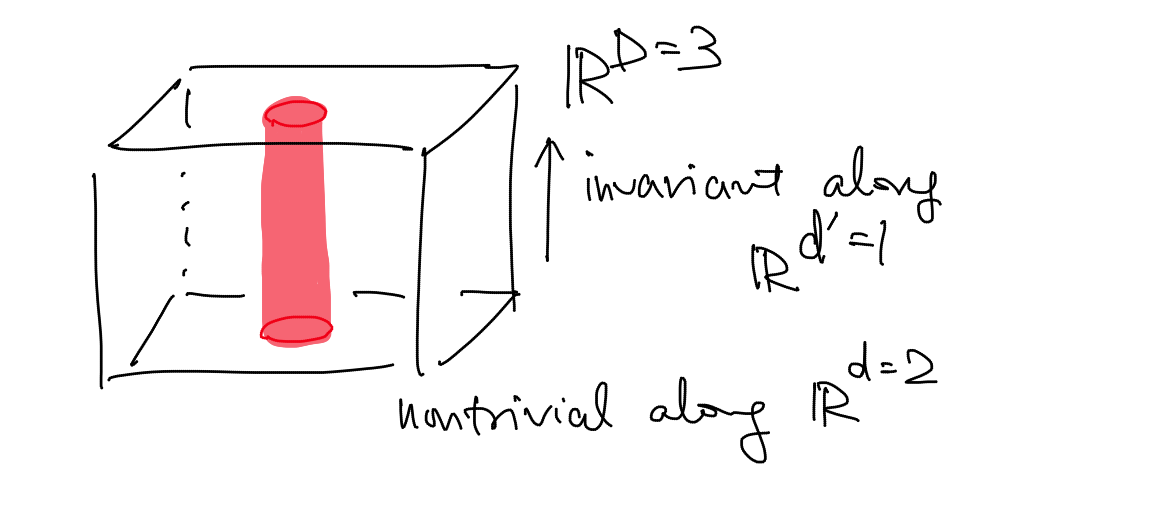
\includegraphics[width=0.7\textwidth]{codimension.png}
  \caption{A codimension-2 object in $\bR^3$ is string-like. }
  \label{fig:codimension}
\end{figure}

Now, in order not to cost an infinite amount of energy in the asymptotically far region,
most of the region of $\bR^d$ needs to map to very close to a point in the target space $X$.
We take this point the basepoint of $X$,
and then such a map is given essentially by a map from $S^d$.
See Fig.~\ref{fig:smoothsoliton}.


\begin{figure}[h]
\centering
  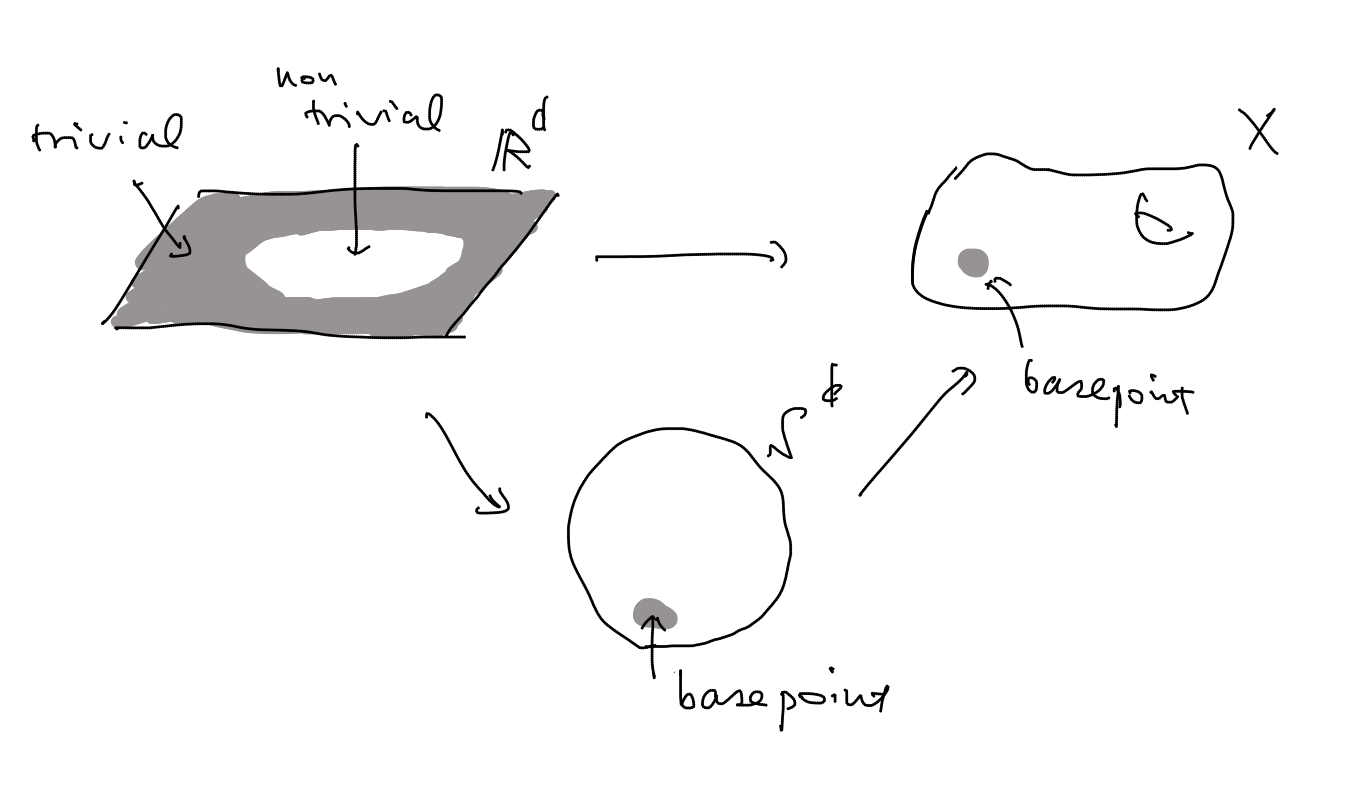
\includegraphics[width=0.7\textwidth]{smoothsoliton.png}
  \caption{A smooth, finite-energy, codimension-$d$ configuration is given by a map $S^d\to X$. }
  \label{fig:smoothsoliton}
\end{figure}

Such a configuration then determines a homotopy class $ [f]\in \pi_d(X)$.
If $[f]$ is nonzero, it cannot be removed by a continuous process,
and therefore it provides a \emph{topologically conserved charge},
and a configuration with such a topologically conserved charge is called a \emph{topological soliton}.

\begin{example}
With codimension-$3$ and the target space $S^3$, we have a Skyrmion whose charge is given by $\pi_3(S^3)=\bZ$.
\end{example}

This was first introduced by Skyrme\footnote{%
In Japan the word Skyrmion is sometimes pronounced as [\textipa{skirmion}] but I think [\textipa{sk@:mion}] is the more correct one;
after all, T. H. R. Skyrme was a British person, and I consider [\textipa{skirmion}] a hypercorrection.
As for the Ising model, I think we should use [\textipa{i:zi\ng}] instead of [\textipa{aizi\ng}],
since E. Ising is a German.
Speaking of pronunciation of names common in our field, 
the pronunciation of K\"allen in K\"allen-Lehmann spectral representation is also tricky.
I often heard high-energy physicists above my generation to pronounce it as [\textipa{tS\ae len}] or something like that.
K\"allen was Swedish,
K\"allen's grandchild was doing string theory, and I met him a couple of times.
He told me the correct pronunciation, which sounded to me  along the line of [\textipa{S\ae lien}],
which was quite different from what the Wikipedia page about the standard Swedish pronunciation.
} \cite{Skyrme:1961vq,Skyrme:1962vh} in the context of a nucleon as a soliton in the meson field.

\begin{example}
With codimension-$2$ and the target space $S^2$, we have a baby Skyrmion whose charge is given by $\pi_2(S^2)=\bZ$.
A baby Skyrmion is often simply called  Skyrmion.
\end{example}

A quick internet search gives me tons of experimental realizations of Skyrmions, 
but most of them seem to be about baby Skyrmions. 

\begin{example}
With codimension-$3$ and the target space $S^2$, we have a Hopfion, whose charge is given by $\pi_3(S^2)=\bZ$.
\end{example}

Again a quick internet search gives me some experimental realizations of Hopfions.
Another notable point is that a Hopfion charge is more subtle than a Skyrmion charge;
if you are interested, you should consult a very recent paper \cite{Chen:2022cyw},\footnote{%
I am mentioning this because I was the proud committee chair of the PhD defense of the junior author of this paper.
}
which pointed out that the Hopfion charge is associated to a non-invertible symmetry,
a hot topic in recent years.


\subsubsection{Solitons with core, better known as topological defects}

Next let us have a look at what can be called with \emph{solitons with core}.
Consider a situation where we have a codimension-$d$ configuration
with a map to the target space $X$, where $X$ is the space of order parmeters, say.
Here we consider a situation illustrated in Fig.~\ref{fig:withcore},
where we have a map \emph{outside} of a core region $U\subset \bR^d$.
So we have a map \begin{equation}
f: \bR\setminus  U \to X.
\end{equation}

\begin{figure}[h]
\centering
  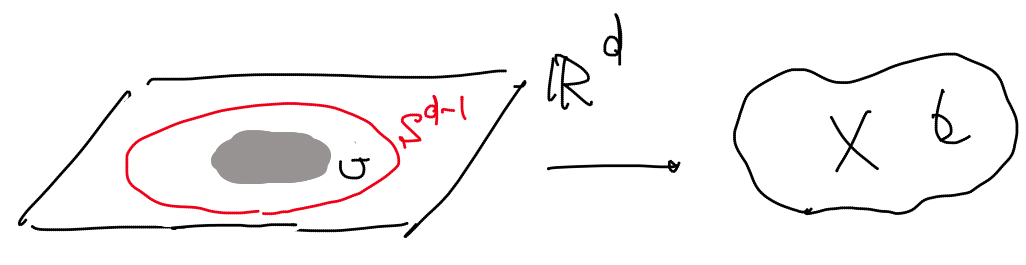
\includegraphics[width=0.6\textwidth]{withcore.png}
  \caption{A codimension-$d$ configuration with `core', given by a map $S^{d-1}\to X$. }
  \label{fig:withcore}
\end{figure}

In this case the nontriviality of such a map is measured by the homotopy class $[f]\in \pi_{d-1}(X)$
of the map $f: S^{d-1}\to X$.
Note the difference to the topological charge measured by  $\pi_d(X)$ of a smooth codimension-$d$ soliton
we discussed above.

Note that if $[f]$ is nontrivial,
it can never be continued smoothly into the entirety of $U$.
Indeed, if so, the resulting map $D^{d}\to X$ provides the homotopy to show $[f]$ is trivial.

When $[f]$ is nontrivial, then, we can't extend the map $f$ continuously to the entirety of $U$.
Inside the region $U$, we assume that some additional physics than 
simply having an order-parameter field parameterized by $X$ is going on.
This can easily happen in physics: usually the space $X$ appears only as a low-energy approximation.
It is then  that in the region $U$ the low-energy approximation breaks down.

Note also that if $[f]$ is nontrivial,
the position dependence of $f$ usually costs an infinite amount energy in the asymptotically far region.
But there are physics situations where this problem might not matter:
\begin{itemize}
\item One is that the experimental setup is finite, so the infinite energy in infinitely large $\bR^d$ might not matter;
\item Another is that when $X=G/H$ and $G$ is associated to a gauge field,
a nontrivial $G$-gauge transformation in the asymptotically far region can remove the position dependence
and therefore the associated infinite amount of energy.
\end{itemize}
In this lecture we therefore neglect these energetic consideration.

\begin{figure}[h]
\centering
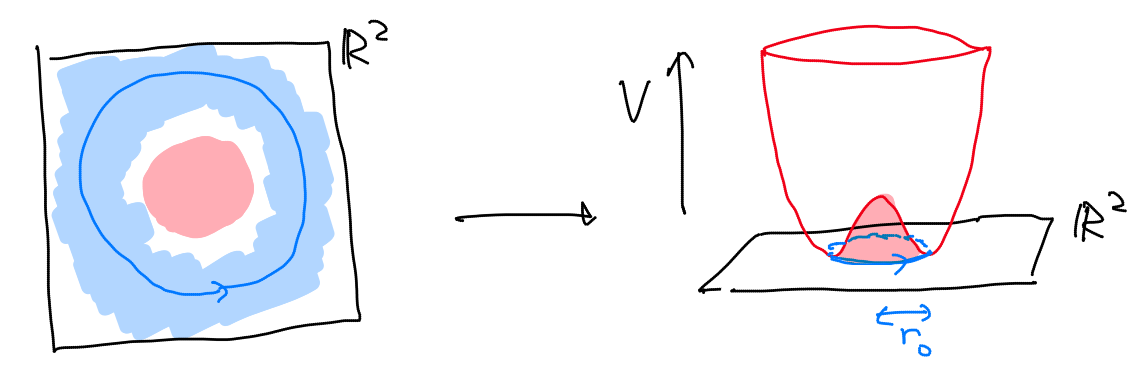
\includegraphics[width=.7\textwidth]{vortex.png}
\caption{A vortex configuration. 
In the asymptotic region, the field values are at the bottom of the potential.
In the core region, the field values come to the origin of the field space.}
\label{fig:vortex}
\end{figure}

An example illustrating the discussion above is when $X=S^1$.
The space $S^1$ of order parameters appears as the space of potential minimum of a wine-bottle potential, as we saw in Sec.~\ref{sec:homogeneous}.
In this case we can consider a field configuration illustrated in Fig.~\ref{fig:vortex}.
In the asymptotically far region, we let the field value  to go around the potential minimum $S^1$,
as we go around the core once. 
In the core region, this $S^1$ in the field space $\bR^2$ needs to shrink. 
This is associated to the additional potential energy, but it is restricted in a finite core region in the space,
and therefore this costs only a finite amount of energy.
Note that the symmetry is broken from $G=U(1)=S^1$ to the trivial group $H=\{e\}$ at the far region,
but the full symmetry is realized at least at a point in the core region,
where the entire  symmetry $G=U(1)$ is unbroken.
In this manner, at the core of the topological soliton, the symmetry is forced to be restored. 


This vortex configuration was first introduced by Abrikosov \cite{Abrikosov:1956sx} in the context of superconductivity 
in condensed matter physics,
and by Nielsen and Olsen \cite{Nielsen:1973cs} in high energy physics. 
By now these vortices are experimentally observed, see Fig.~\ref{fig:vortex-exp}.
\begin{figure}[h]
\centering
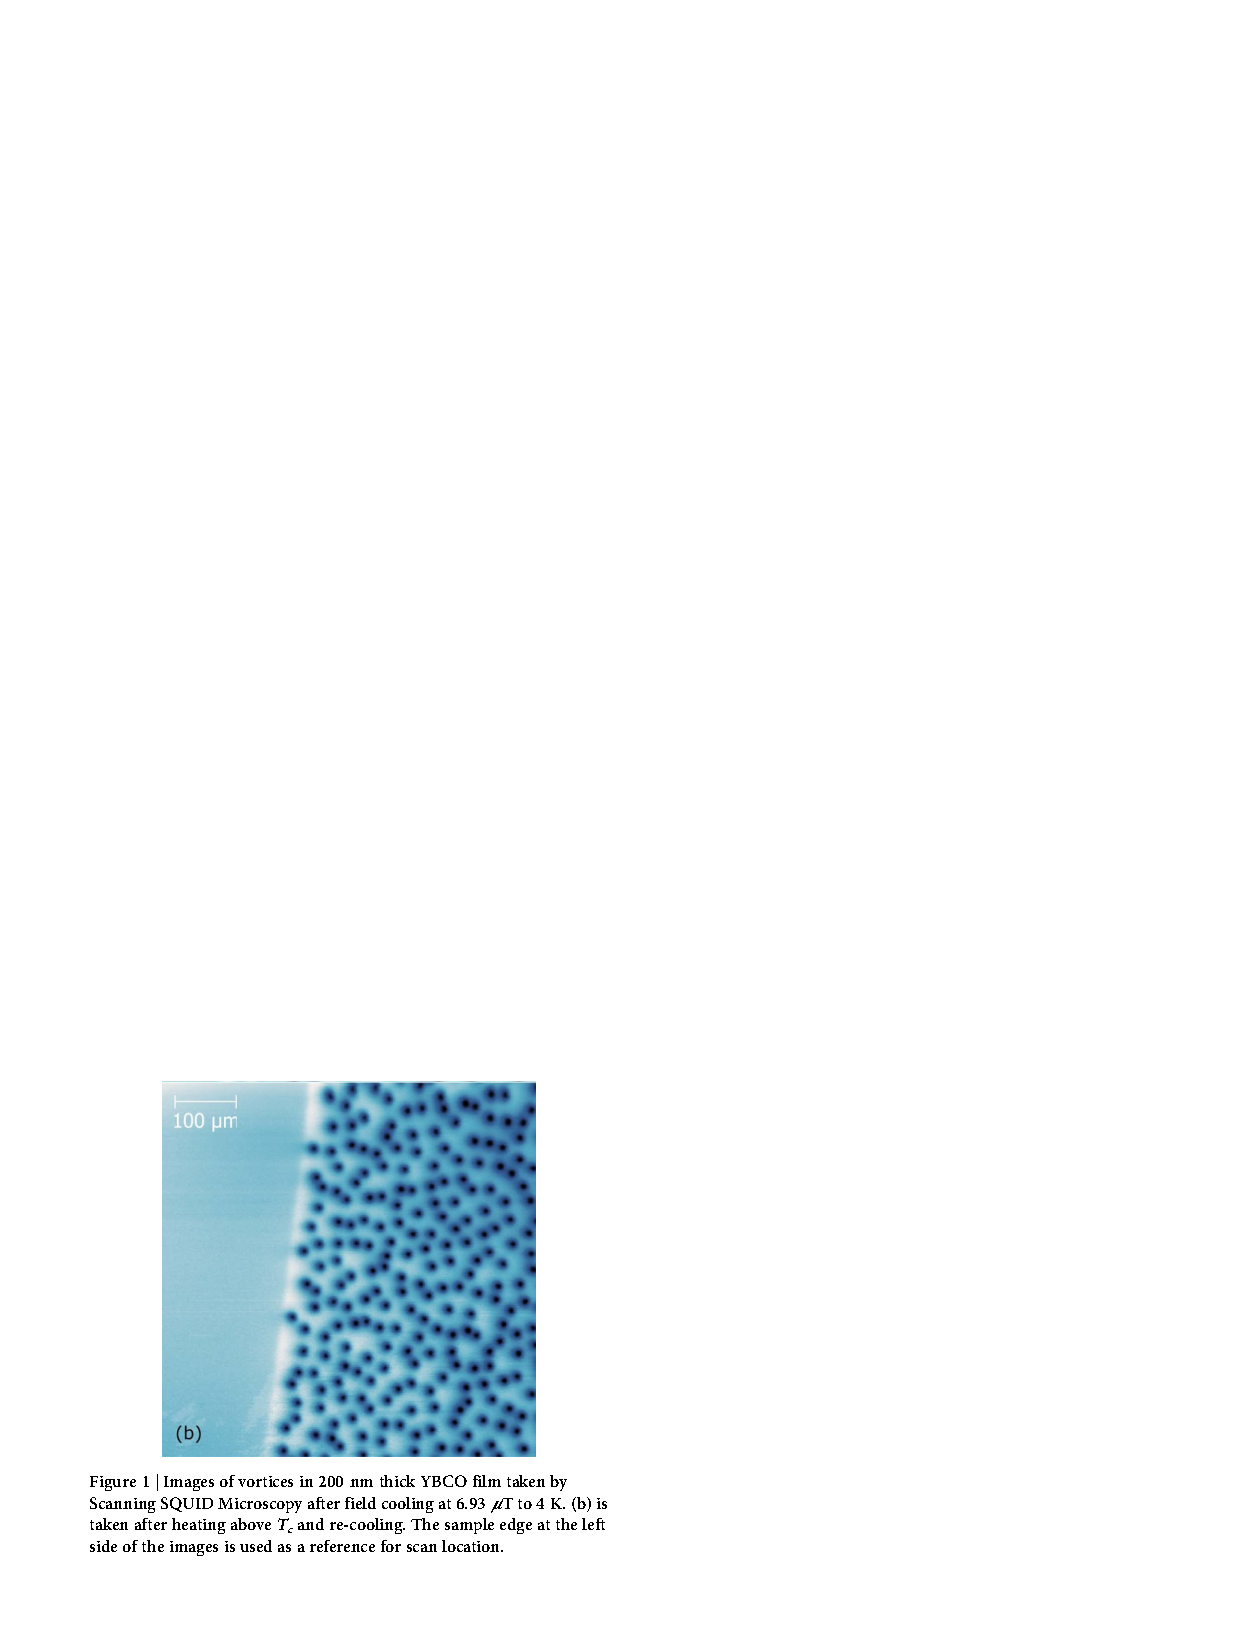
\includegraphics[width=.5\textwidth]{vortices.pdf}
\caption{A scanning SQUID-microscope view of the vortices in a superconducting material.
Taken from \cite{VortexExp}.}
\label{fig:vortex-exp}
\end{figure}
Summarizing, 
\begin{example}
A codimension-2 topological soliton with a core for the parameter space $X=U(1)$,
characterized by $\pi_1(U(1))=\bZ$,
is known as the Abrikosov/Nielsen-Olsen vortex.
\end{example}


Let us further identify this $G=U(1)$ is identified with the electromagnetic $U(1)$.
In this case, we can show that the core region contains a unit magnetic flux in the following manner;
we will give a more traditional approach using the vector potential later.
To measure the magnetic flux topologically,
let us try to put this configuration on an $S^2$, and use the result in Sec.~\ref{sec:bundle-over-sphere}.
We first put this configuration on a large $D^2$, which we consider to be the northern hemisphere.
We have a region $B$ around the equator $L$ 
%(given in blue in Fig.~\ref{fig:R2S2})
where we have a product bundle $B \times S^1$.
For the sake of generality,
let us say that the field value  goes around $S^1$ $N$ times, when we go around the equator once.

We also introduce another $D^2$, which we use as the southern hemisphere.
On it, we consider a trivial bundle $D^2\times S^1$ and a constant section.
To paste the two hemispheres so that the sections match, 
we need to use a $U(1)$ gauge transformation $g:S^1\to S^1$ which also goes around $S^1$ $N$ times.
This means that on the resulting $S^2$, the $U(1)$ bundle
is characterized by $N\in \pi_1(S^1)\simeq \bZ$,
and therefore has the magnetic charge $N$.
See Fig.~\ref{fig:vortex-flux} for an illustration.

\begin{figure}[h]
\centering
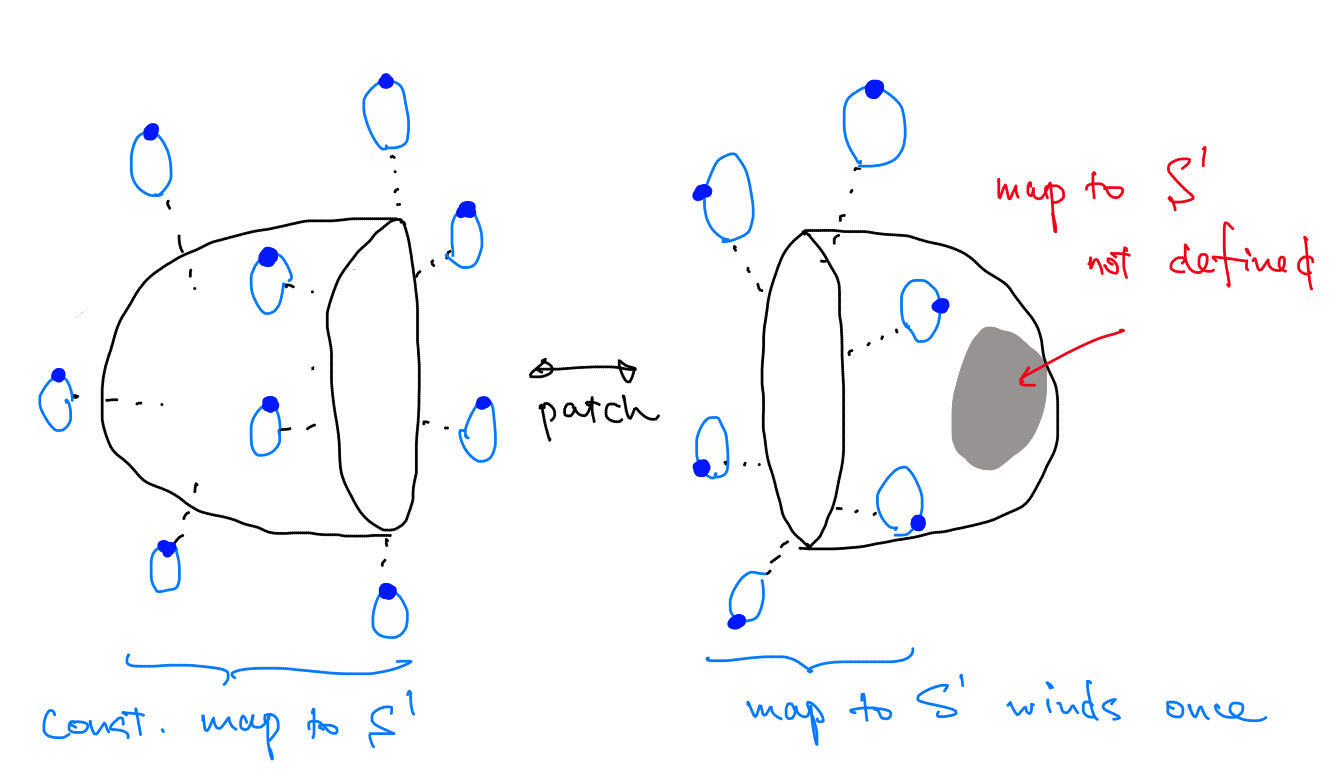
\includegraphics[width=.8\textwidth]{vortex-flux.png}
\caption{To measure the magnetic flux, we can put a vortex configuration on $S^2$.
This requires a nontrivial gauge transformation around the equator.}
\label{fig:vortex-flux}
\end{figure}


Although not directly relevant to nature,
at least at the mathematical level we can replace $\pi_1(U(1))=\bZ$ with $\pi_3(SU(2))$,
and consider a codimension-4 particle in a $(4+1)$-dimensional system:
\begin{example}
A codimension-4 topological soliton with a core for the parameter space $X=SU(2)$
can be considered.
\end{example}
For example, a D0-brane within a stack of D4-branes has such a realization,
where D$p$-brane is a $(p+1)$-dimensional solitonic objects in string theory.

Note that our argument in Sec.~\ref{sec:long-exact-and-bundles} 
shows that the core of this soliton has the instanton charge $1$, 
again characterized by the same $\pi_3(SU(2))=\bZ$.
For this reason this is often called an `instanton-particle' in string theory.


Our final example is the following:
\begin{example}
A codimension-3 topological soliton with a core for the parameter space $X=S^2$
is known as 't Hooft-Polyakov monopole.
\end{example}
This was first introduced by 't Hooft \cite{tHooft:1974kcl} and Polyakov \cite{Polyakov:1974ek}.
When we regard $S^2=SU(2)/U(1)$
and consider a gauge theory setup where we have a larger group $SU(2)$ broken to $U(1)$,
and identify $U(1)$ as the electromagnetic gauge group,
it has a magnetic charge on $S^2$,
whose charge is characterized by Proposition~\ref{prop:connecting-and-bundle} 
via the image of $\pi_2(SU(2)/U(1))$ to $\pi_1(U(1))$ in the part of
 the long exact sequence of  homotopy groups associated to the bundle $U(1)\to SU(2)\to SU(2)/U(1)$: \begin{equation}
 \pi_2(SU(2)/U(1)) \to \pi_1(U(1)) \to \pi_1(SU(2))\to \pi_1(SU(2)/U(1))
\end{equation} which is \begin{equation}
 \bZ \to \bZ \to 0 \to 0.
\end{equation}
The exactness forces the first map to be the identity.
Therefore, the minimal 't Hooft-Polyakov monopole characterized by $1\in \pi_2(S^2)=\bZ$
has the unit magnetic charge $1\in \pi_1(U(1))$.

In contrast, if we regard $S^2=SO(3)/SO(2)$
and identify $SO(2)$ as the electromagnetic gauge group,
the magnetic charge is characterized by the same token by studying \begin{equation}
 \pi_2(SU(2)/U(1)) \to \pi_1(SO(2)) \to \pi_1(SO(3)) \to \pi_1(SU(2)/U(1))
\end{equation} which is \begin{equation}
 \bZ \to \bZ \to \bZ_2 \to 0.
\end{equation}
The exactness forces the first map to be a multiplication by $2$.
Therefore, the minimal 't Hooft-Polyakov monopole characterized by $1\in \pi_2(S^2)=\bZ$
has the magnetic charge $2\in \pi_1(SO(2))$, which has twice the minimal value.

This subtle difference of the magnetic charge of the 't Hooft-Polyakov monopole by a factor of two
between an $SU(2)$ gauge theory and an $SO(3)$ gauge theory
 plays an important role in the modern study of topological properties of gauge theories.
 See e.g.~\cite{Aharony:2013hda}.

\subsubsection{A remark and suggested questions}

Note that $\pi_d(X)$ can correspond to a codimension-$d$ texture (i.e.~a topological soliton without core)
and also to a codimension-$(d+1)$ topological defect (i.e.~a topological soliton with core).
In general they can coexist, but I do not know any concrete examples.

\begin{question}
The superfluid Helium 3 A-phase and B-phase have various topological solitons characterized by $\pi_d(G/H_\text{A})$
and $\pi_d(G/H_\text{B})$ we discussed in Example~\ref{ex:helium3}.
Learn about it. 
\end{question}

The description of $\pi_d(G/H_\text{A})$ is a good exercise of the long exact sequence we learned above.
I am not familiar with the status of experimental verification of these predicted topological solitons.

\begin{question}
Look for an experimental paper on a topological soliton, either with or without core, and study it.
\end{question}

\section{Differential forms and de Rham cohomology}
\label{sec:deRham}

\section{Cellular cohomology}

\section{Characteristic classes}

\section{Classifying spaces}

\section{Chern-Simons terms and bordism groups}

\section{K-theory}

\section{Atiyah-Singer index theorem}

\section{Anomalies}

\section{Computing \texorpdfstring{$\pi_4(S^3)$}{pi4(S3)}}

\bibliographystyle{ytamsalpha}
%\baselineskip=.85\baselineskip%\let\ttfamily\relax
%\let\bbb\bibitem\def\bibitem{\itemsep1pt\bbb}
\bibliography{ref}

\end{document}
